\begin{landscape}
\chapter{Visualization}

\section{Data Collection Validation}

In the pre-processing experiment, the method used for collecting and filtering the 1000 Tweets.
To test that the distribution and collection was being done correctly, figures~\ref{fig:preprocessdist} and~\ref{fig:finaldist} where generated.


\begin{figure}[!htb]
\minipage{0.5\textwidth}
  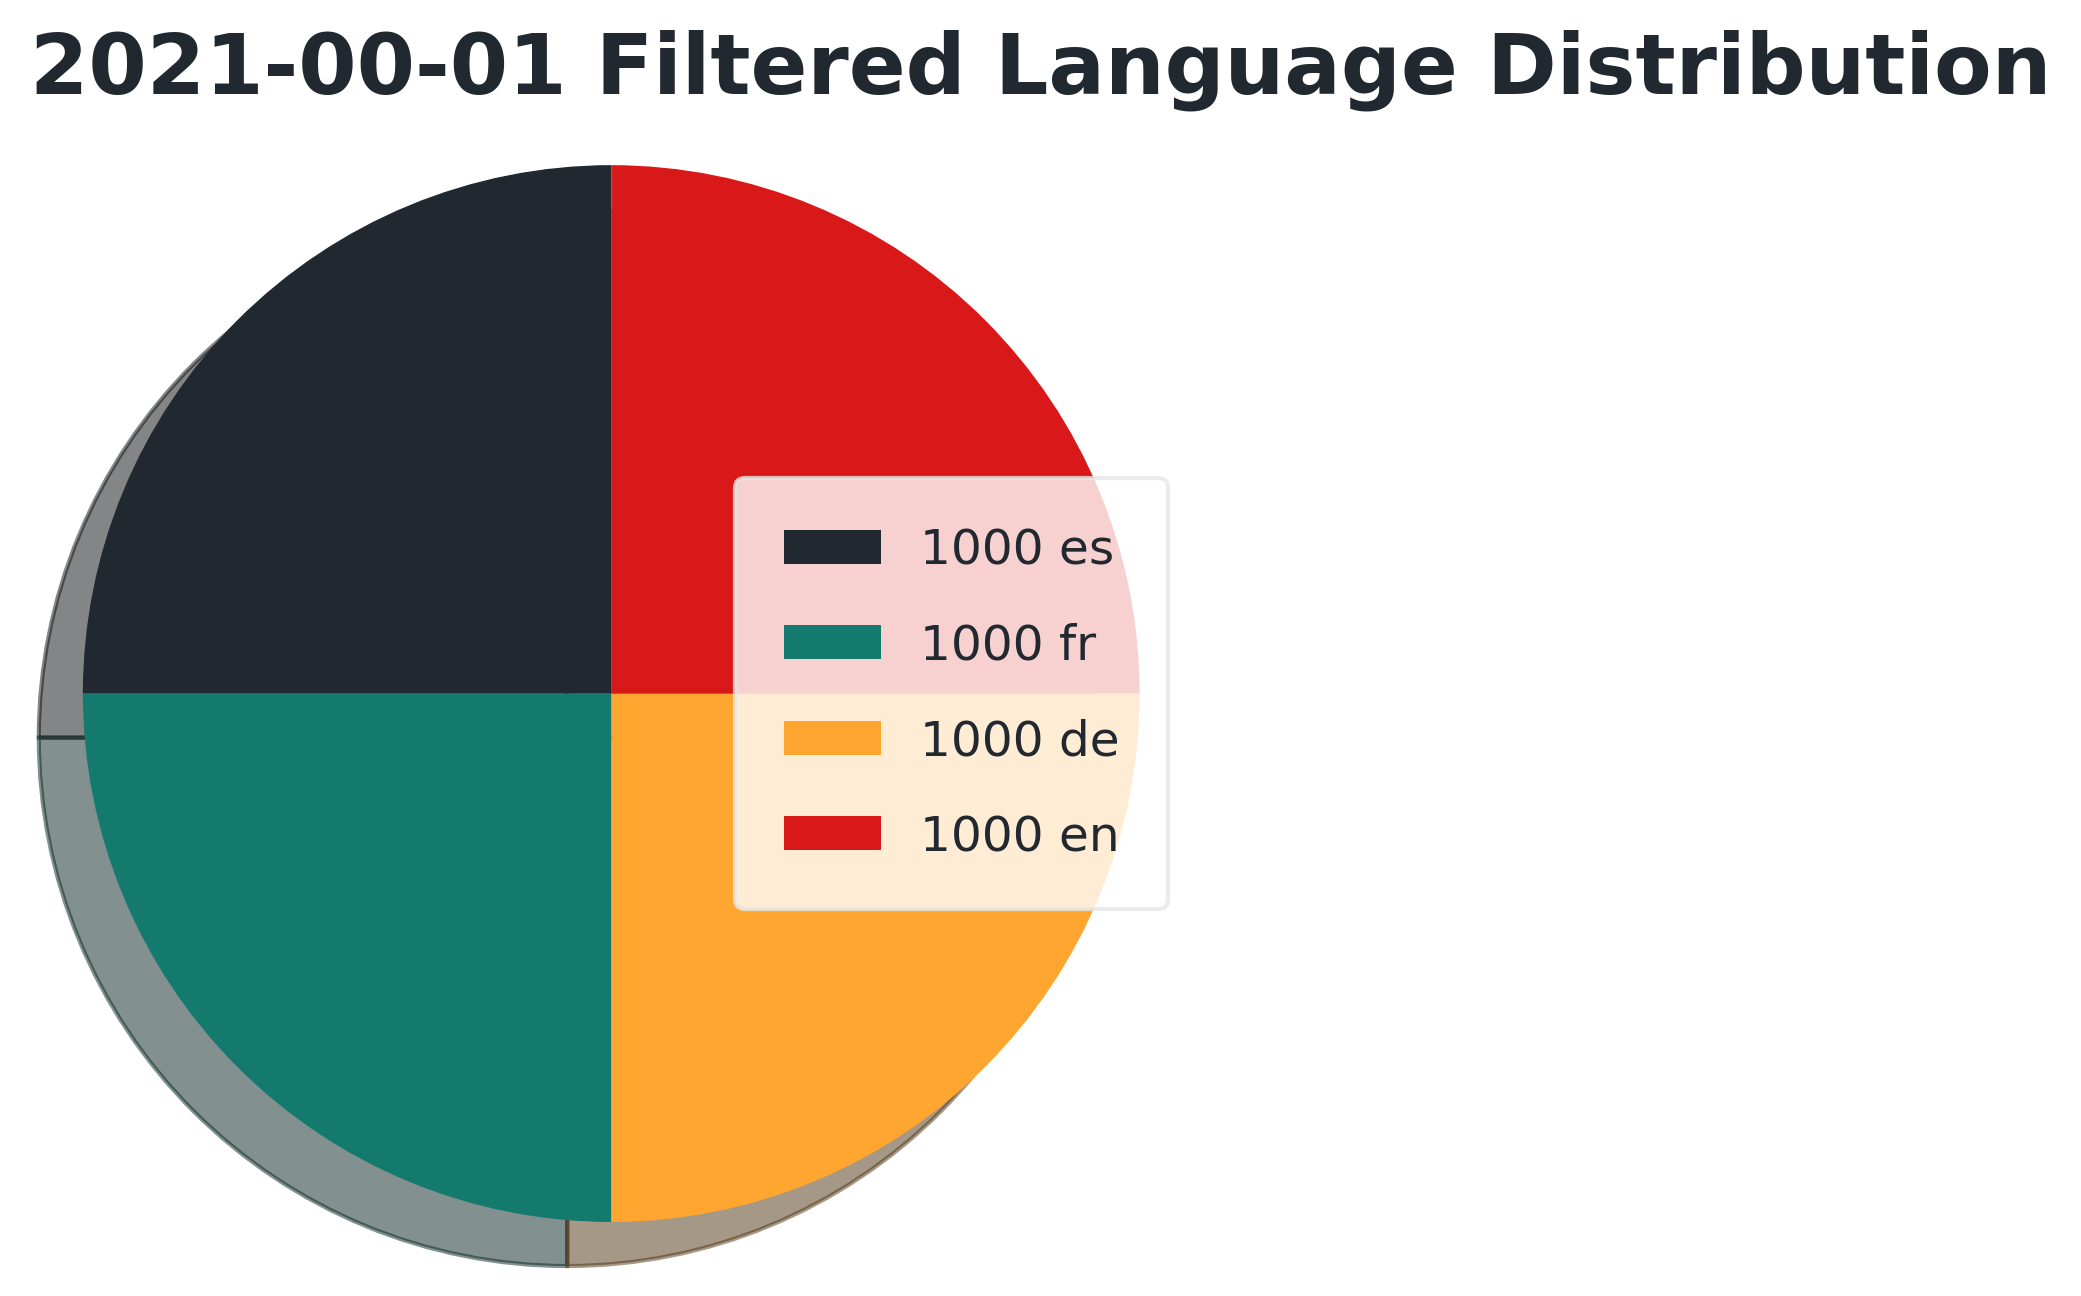
\includegraphics[width=\linewidth]{2021-00-01 Filtered Language Distribution.png}
  \caption[Pre-Process Filtered Language Distribution]{ }
  \label{fig:preprocessdist}
\endminipage\hfill
\minipage{0.5\textwidth}
  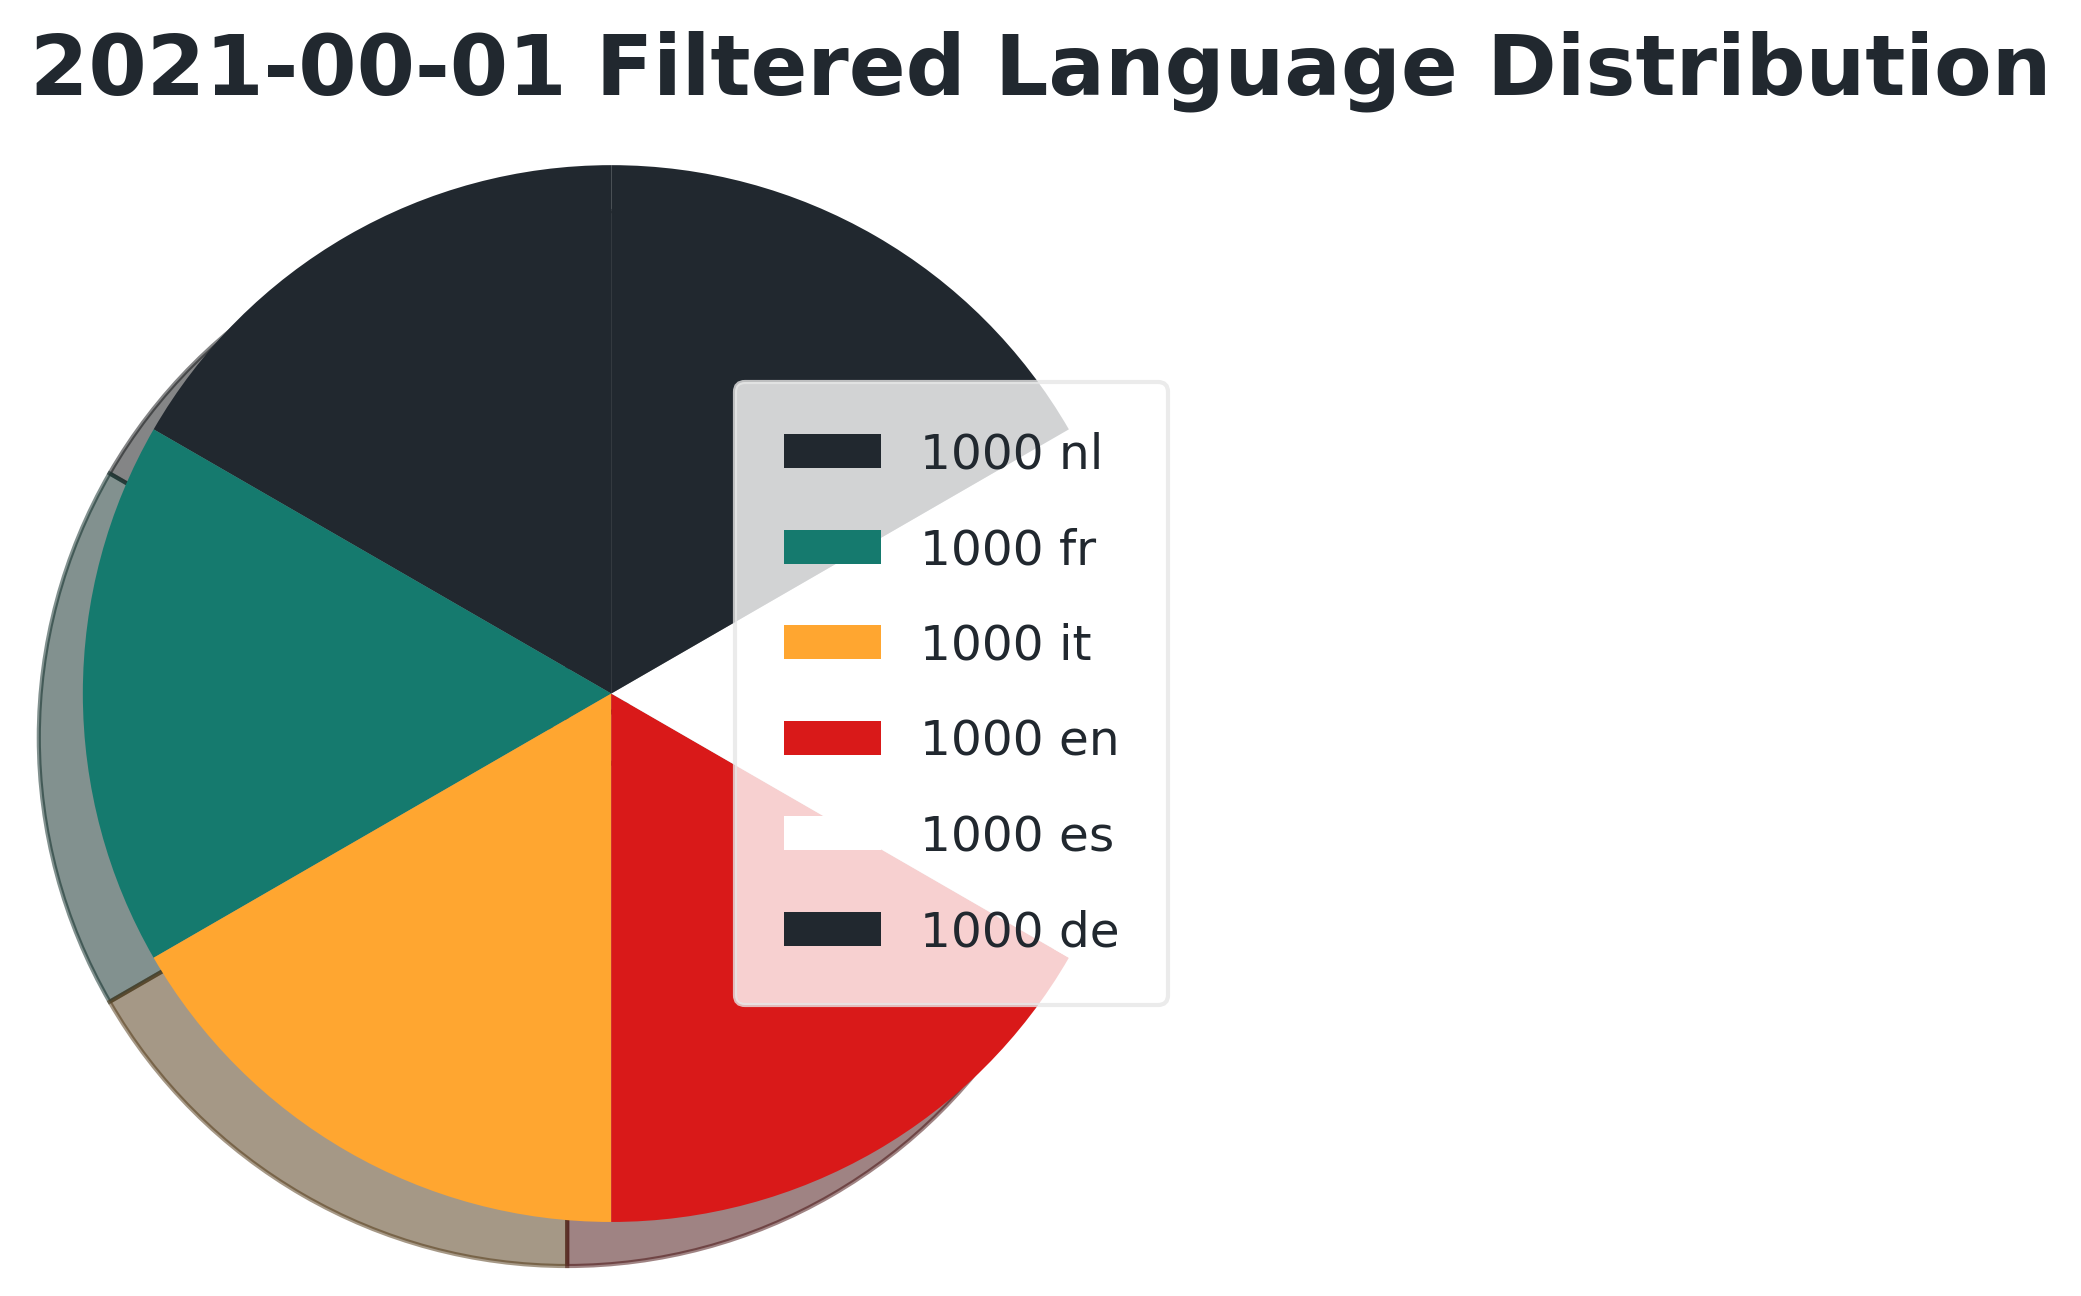
\includegraphics[width=\linewidth]{2021-01-01 Filtered Language Distribution - Final.png}
  \caption[Final Filtered Language Distribution]{ }
  \label{fig:finaldist}
\endminipage
\end{figure}

\newpage

\section{Pre-Processing Effect}

The compound sentiment scores returned from the \ac{VADER} model was averaged and plotted for the 3 dates used in the experiment.
The 4 graphs produced, figures~\ref{fig:EnglishPre} to~\ref{fig:GermanPre}, show a time series graph of each language over the 3 days which are 1 month apart.

\begin{figure}[!htb]
\minipage{0.5\textwidth}
  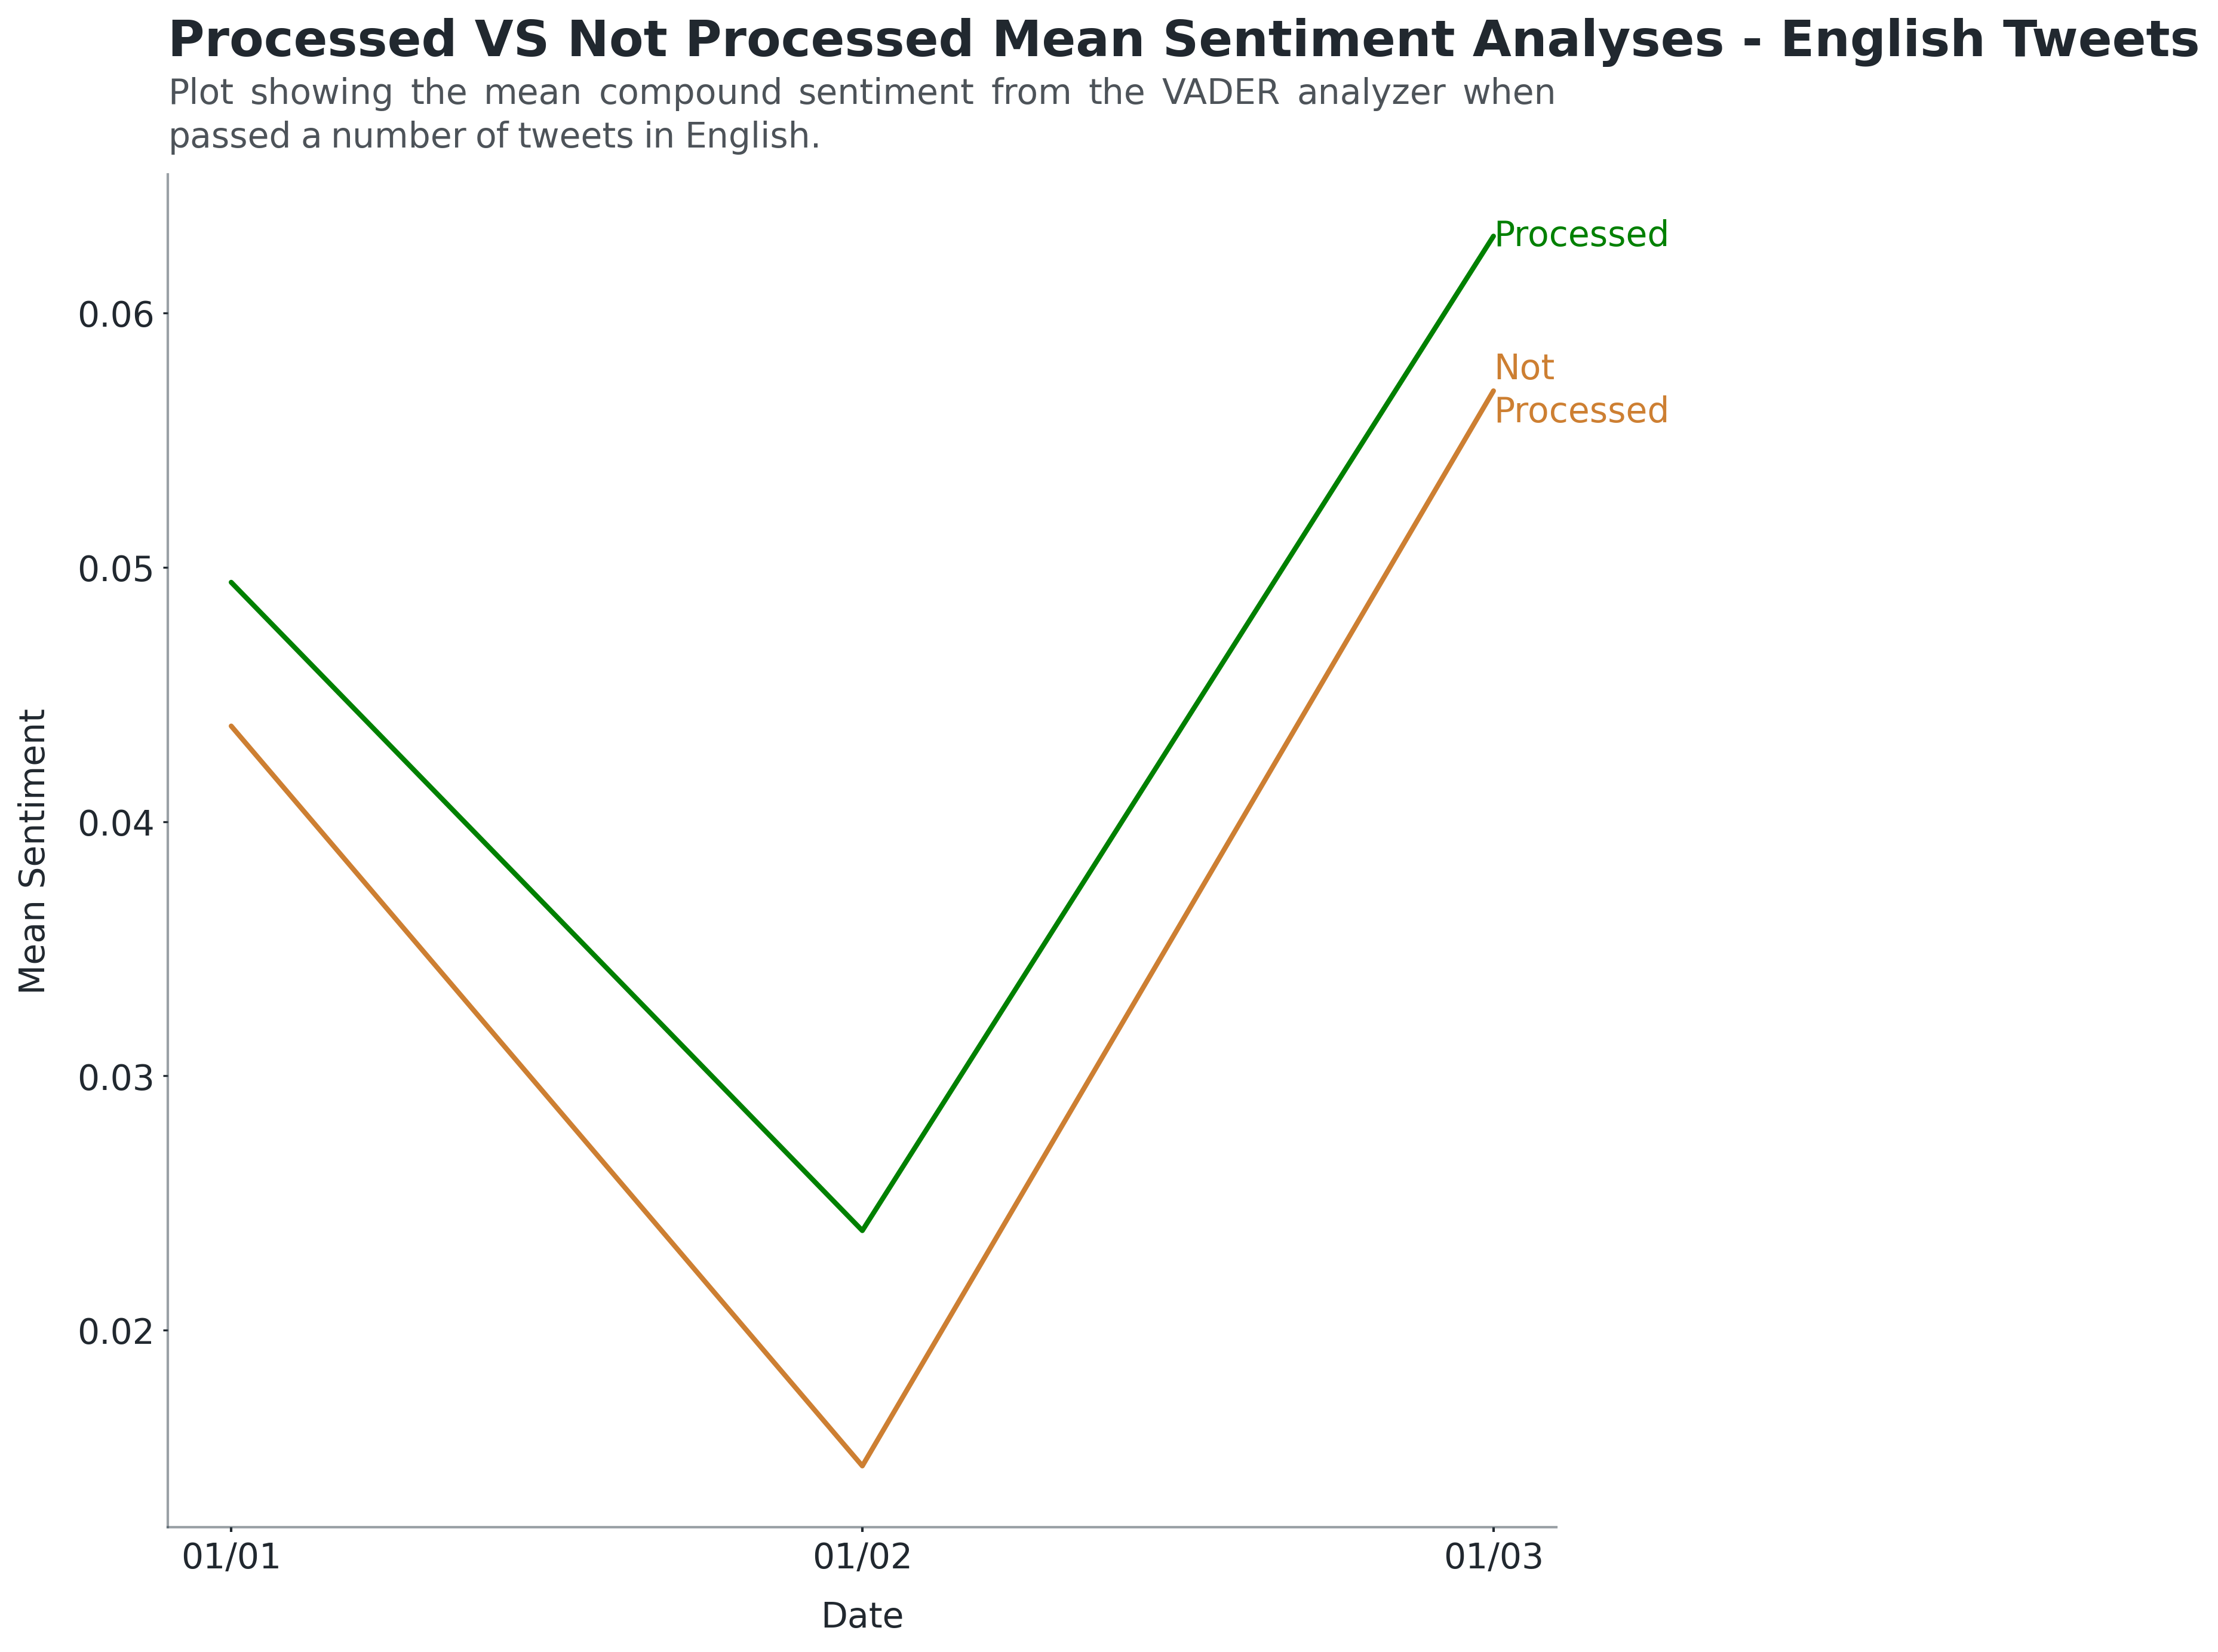
\includegraphics[width=\linewidth]{English Process VS NotProcessed.png}
  \caption[English Process VS NotProcessed]{ }\label{fig:EnglishPre}
\endminipage\hfill
\minipage{0.5\textwidth}
  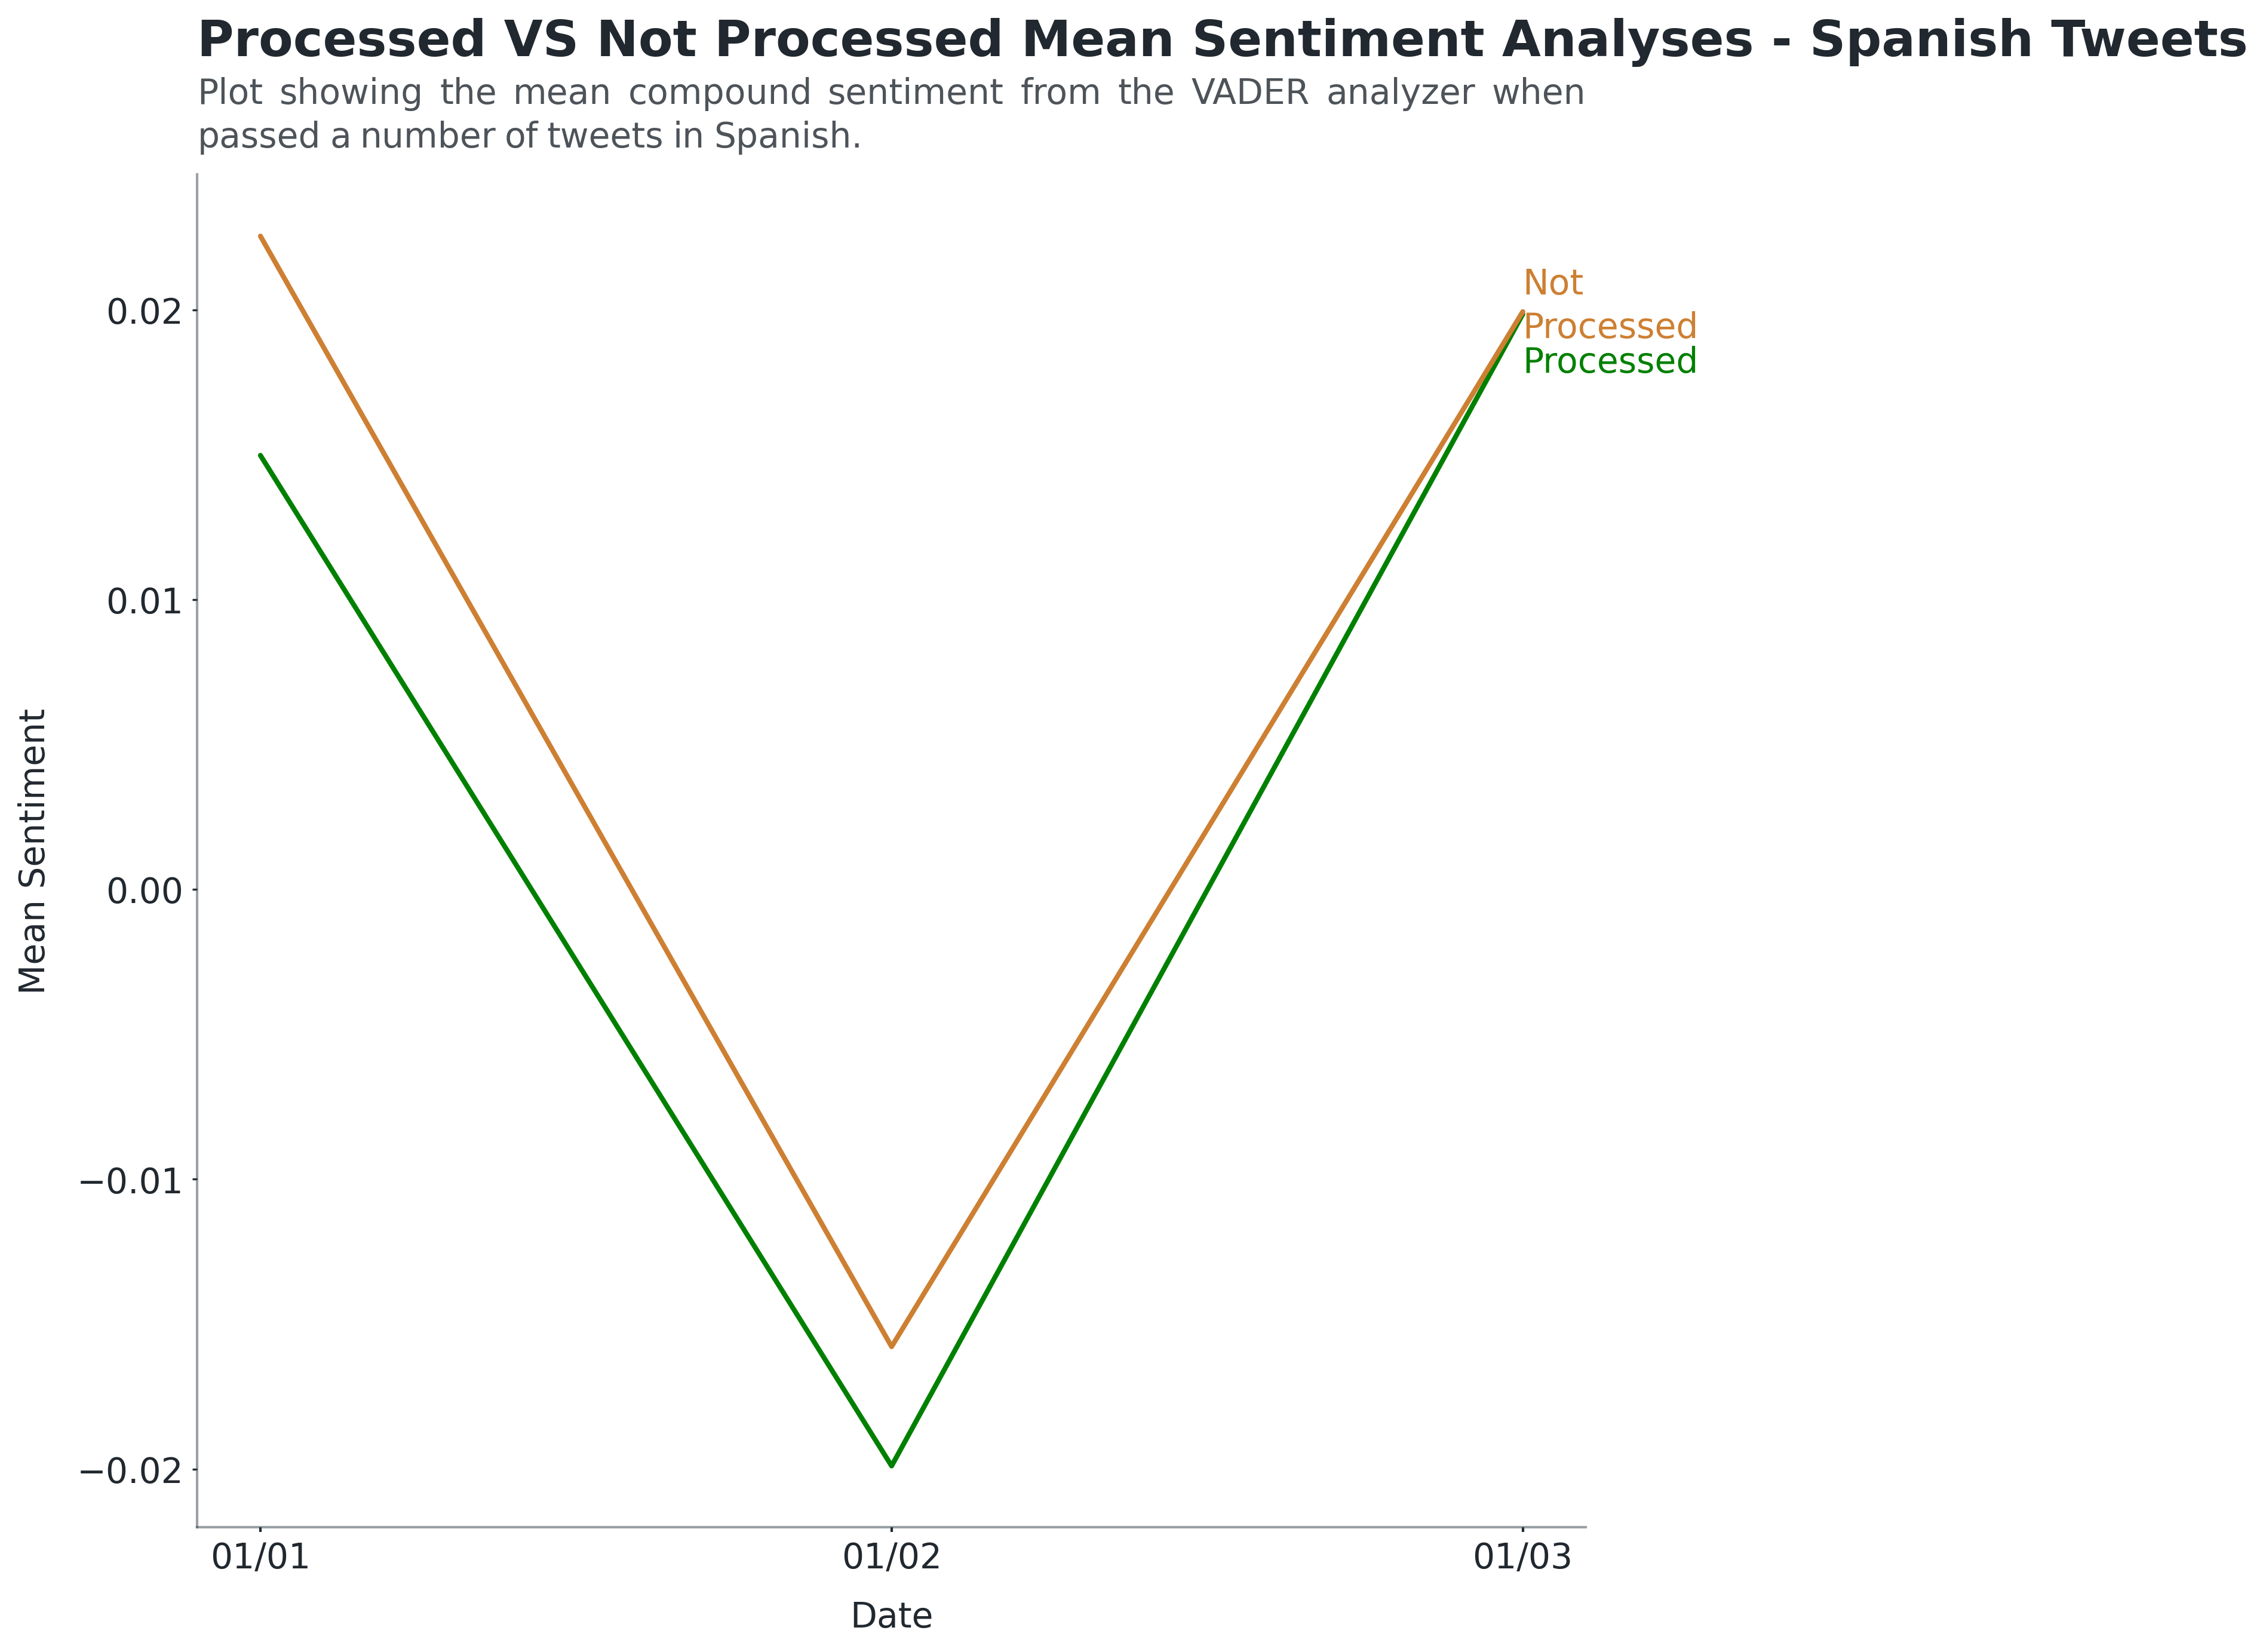
\includegraphics[width=\linewidth]{Spanish Process VS NotProcessed.png}
  \caption[Spanish Process VS NotProcessed]{ }\label{fig:SpanishPre}
\endminipage
\end{figure}
\begin{figure}[!htb]
\minipage{0.5\textwidth}
  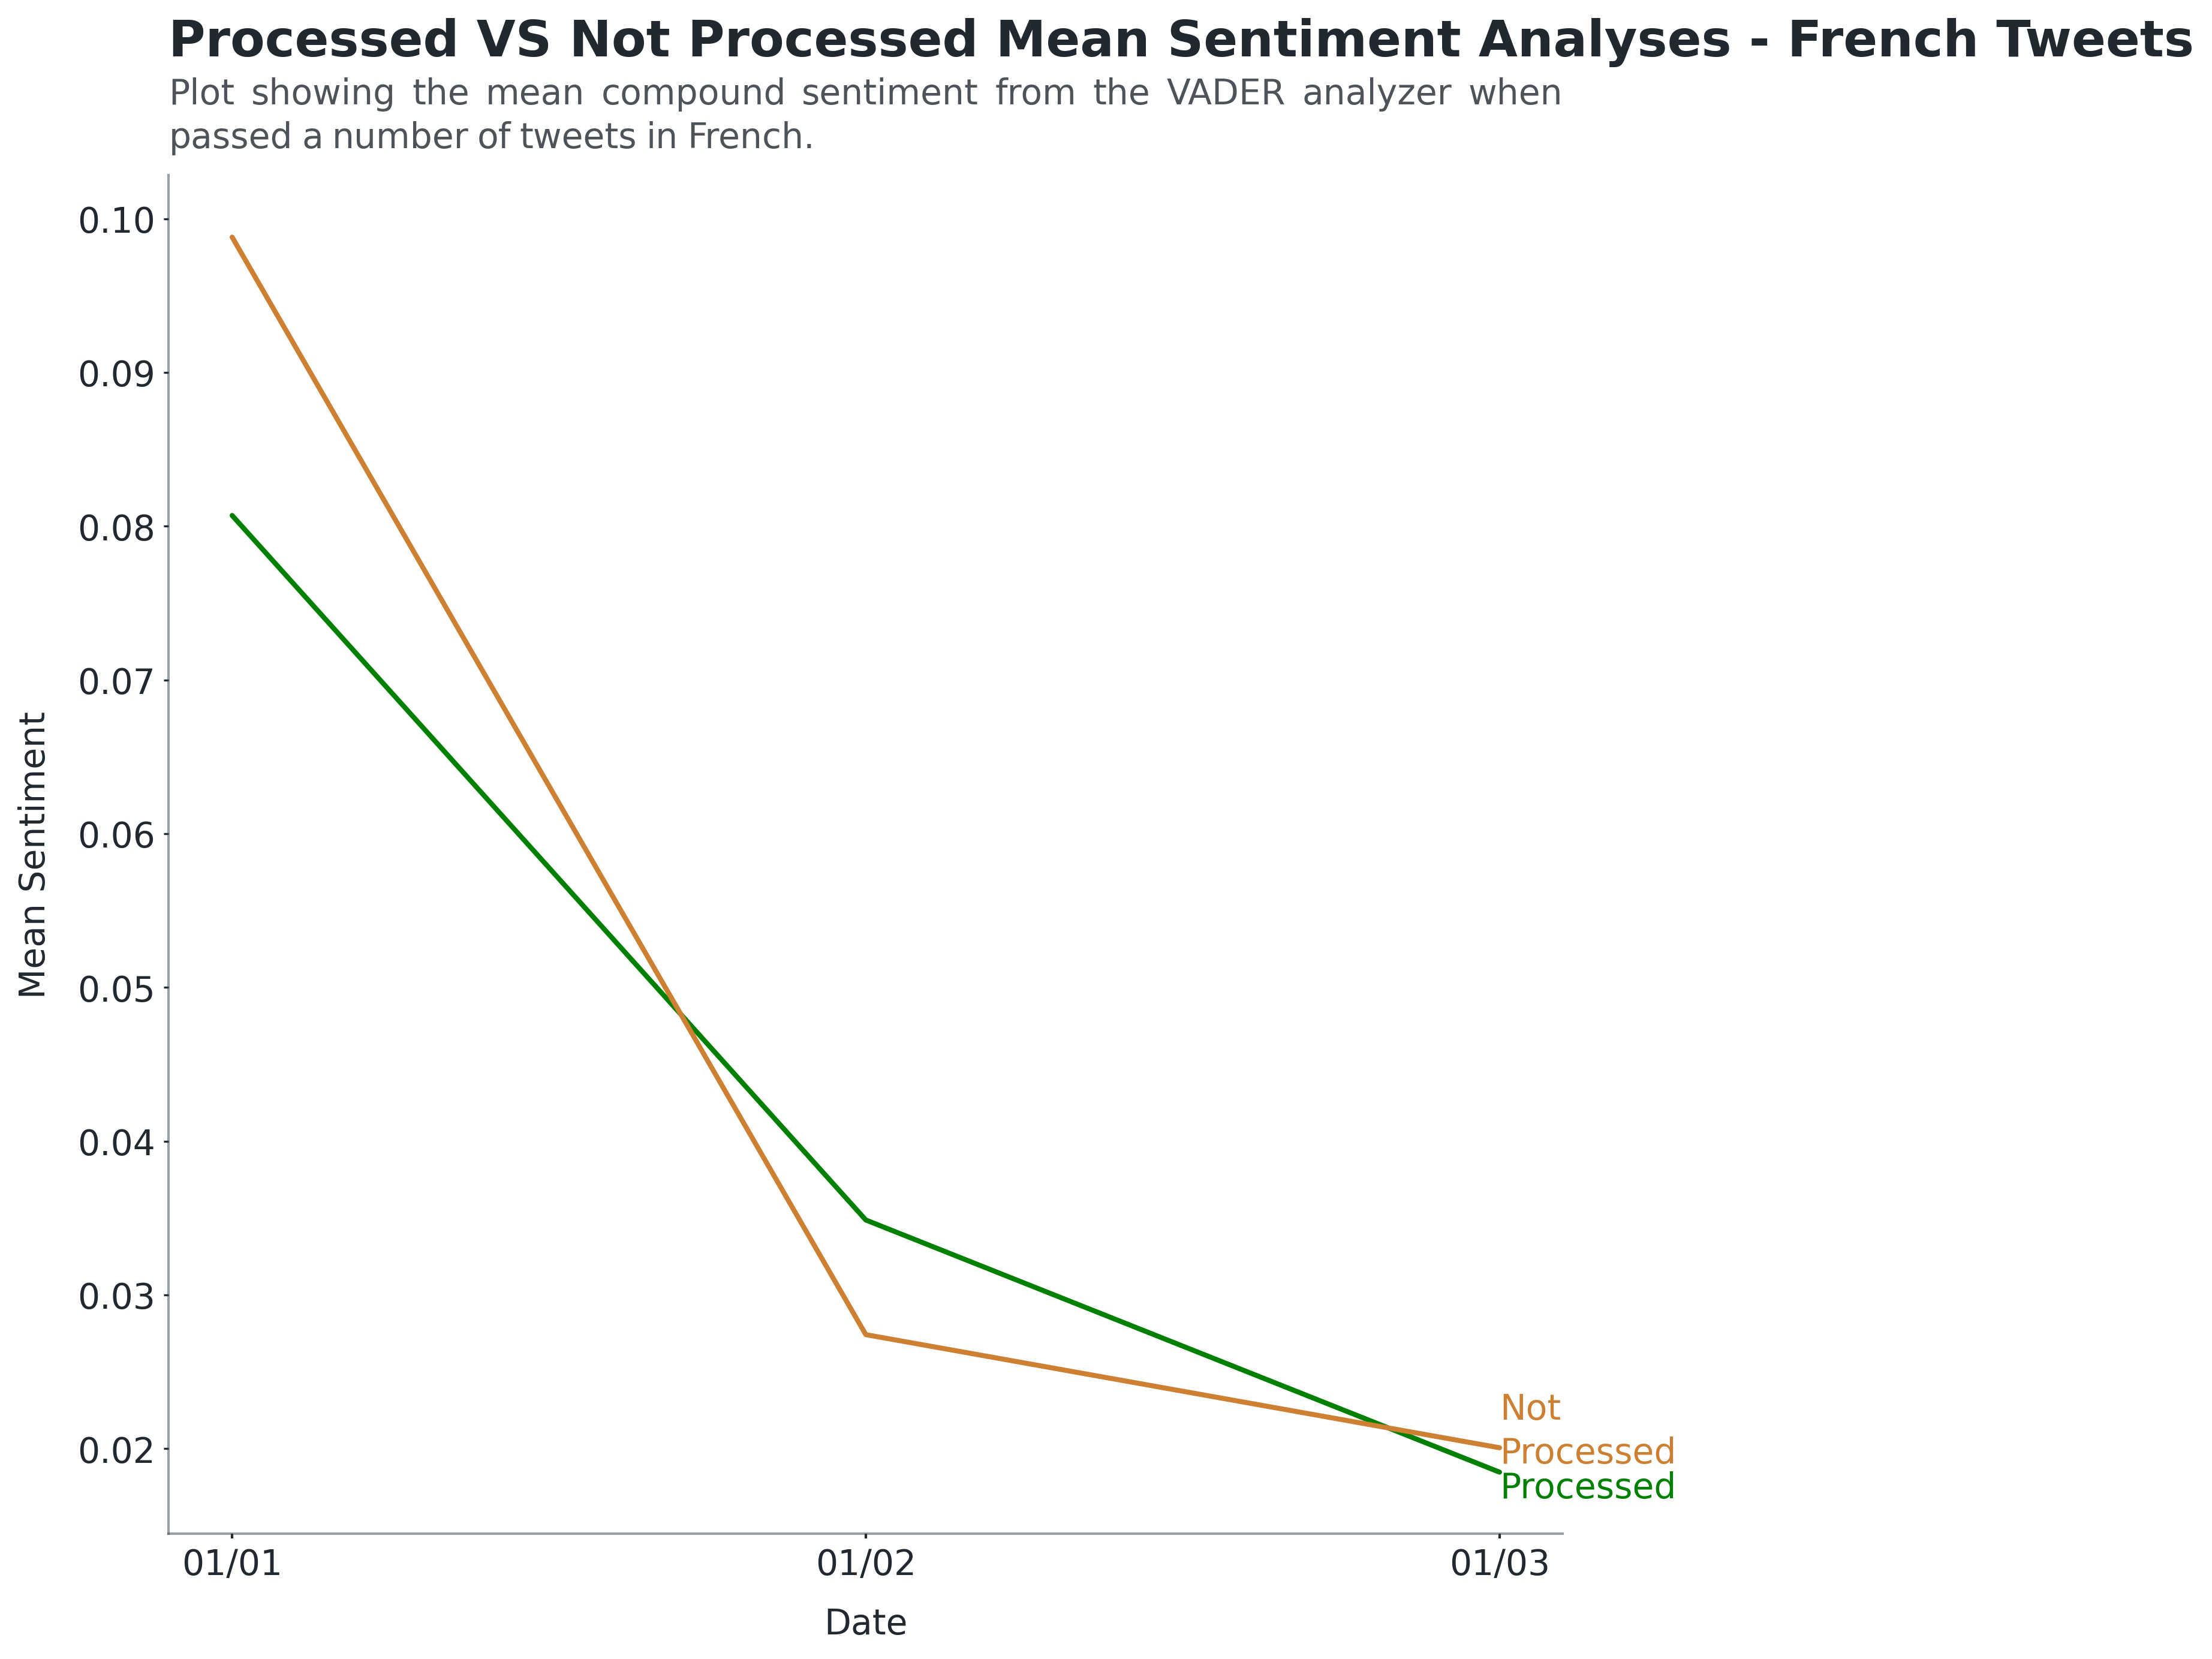
\includegraphics[width=\linewidth]{French Process VS NotProcessed.png}
  \caption[French Process VS NotProcessed]{ }\label{fig:FrenchPre}
\endminipage\hfill
\minipage{0.5\textwidth}
  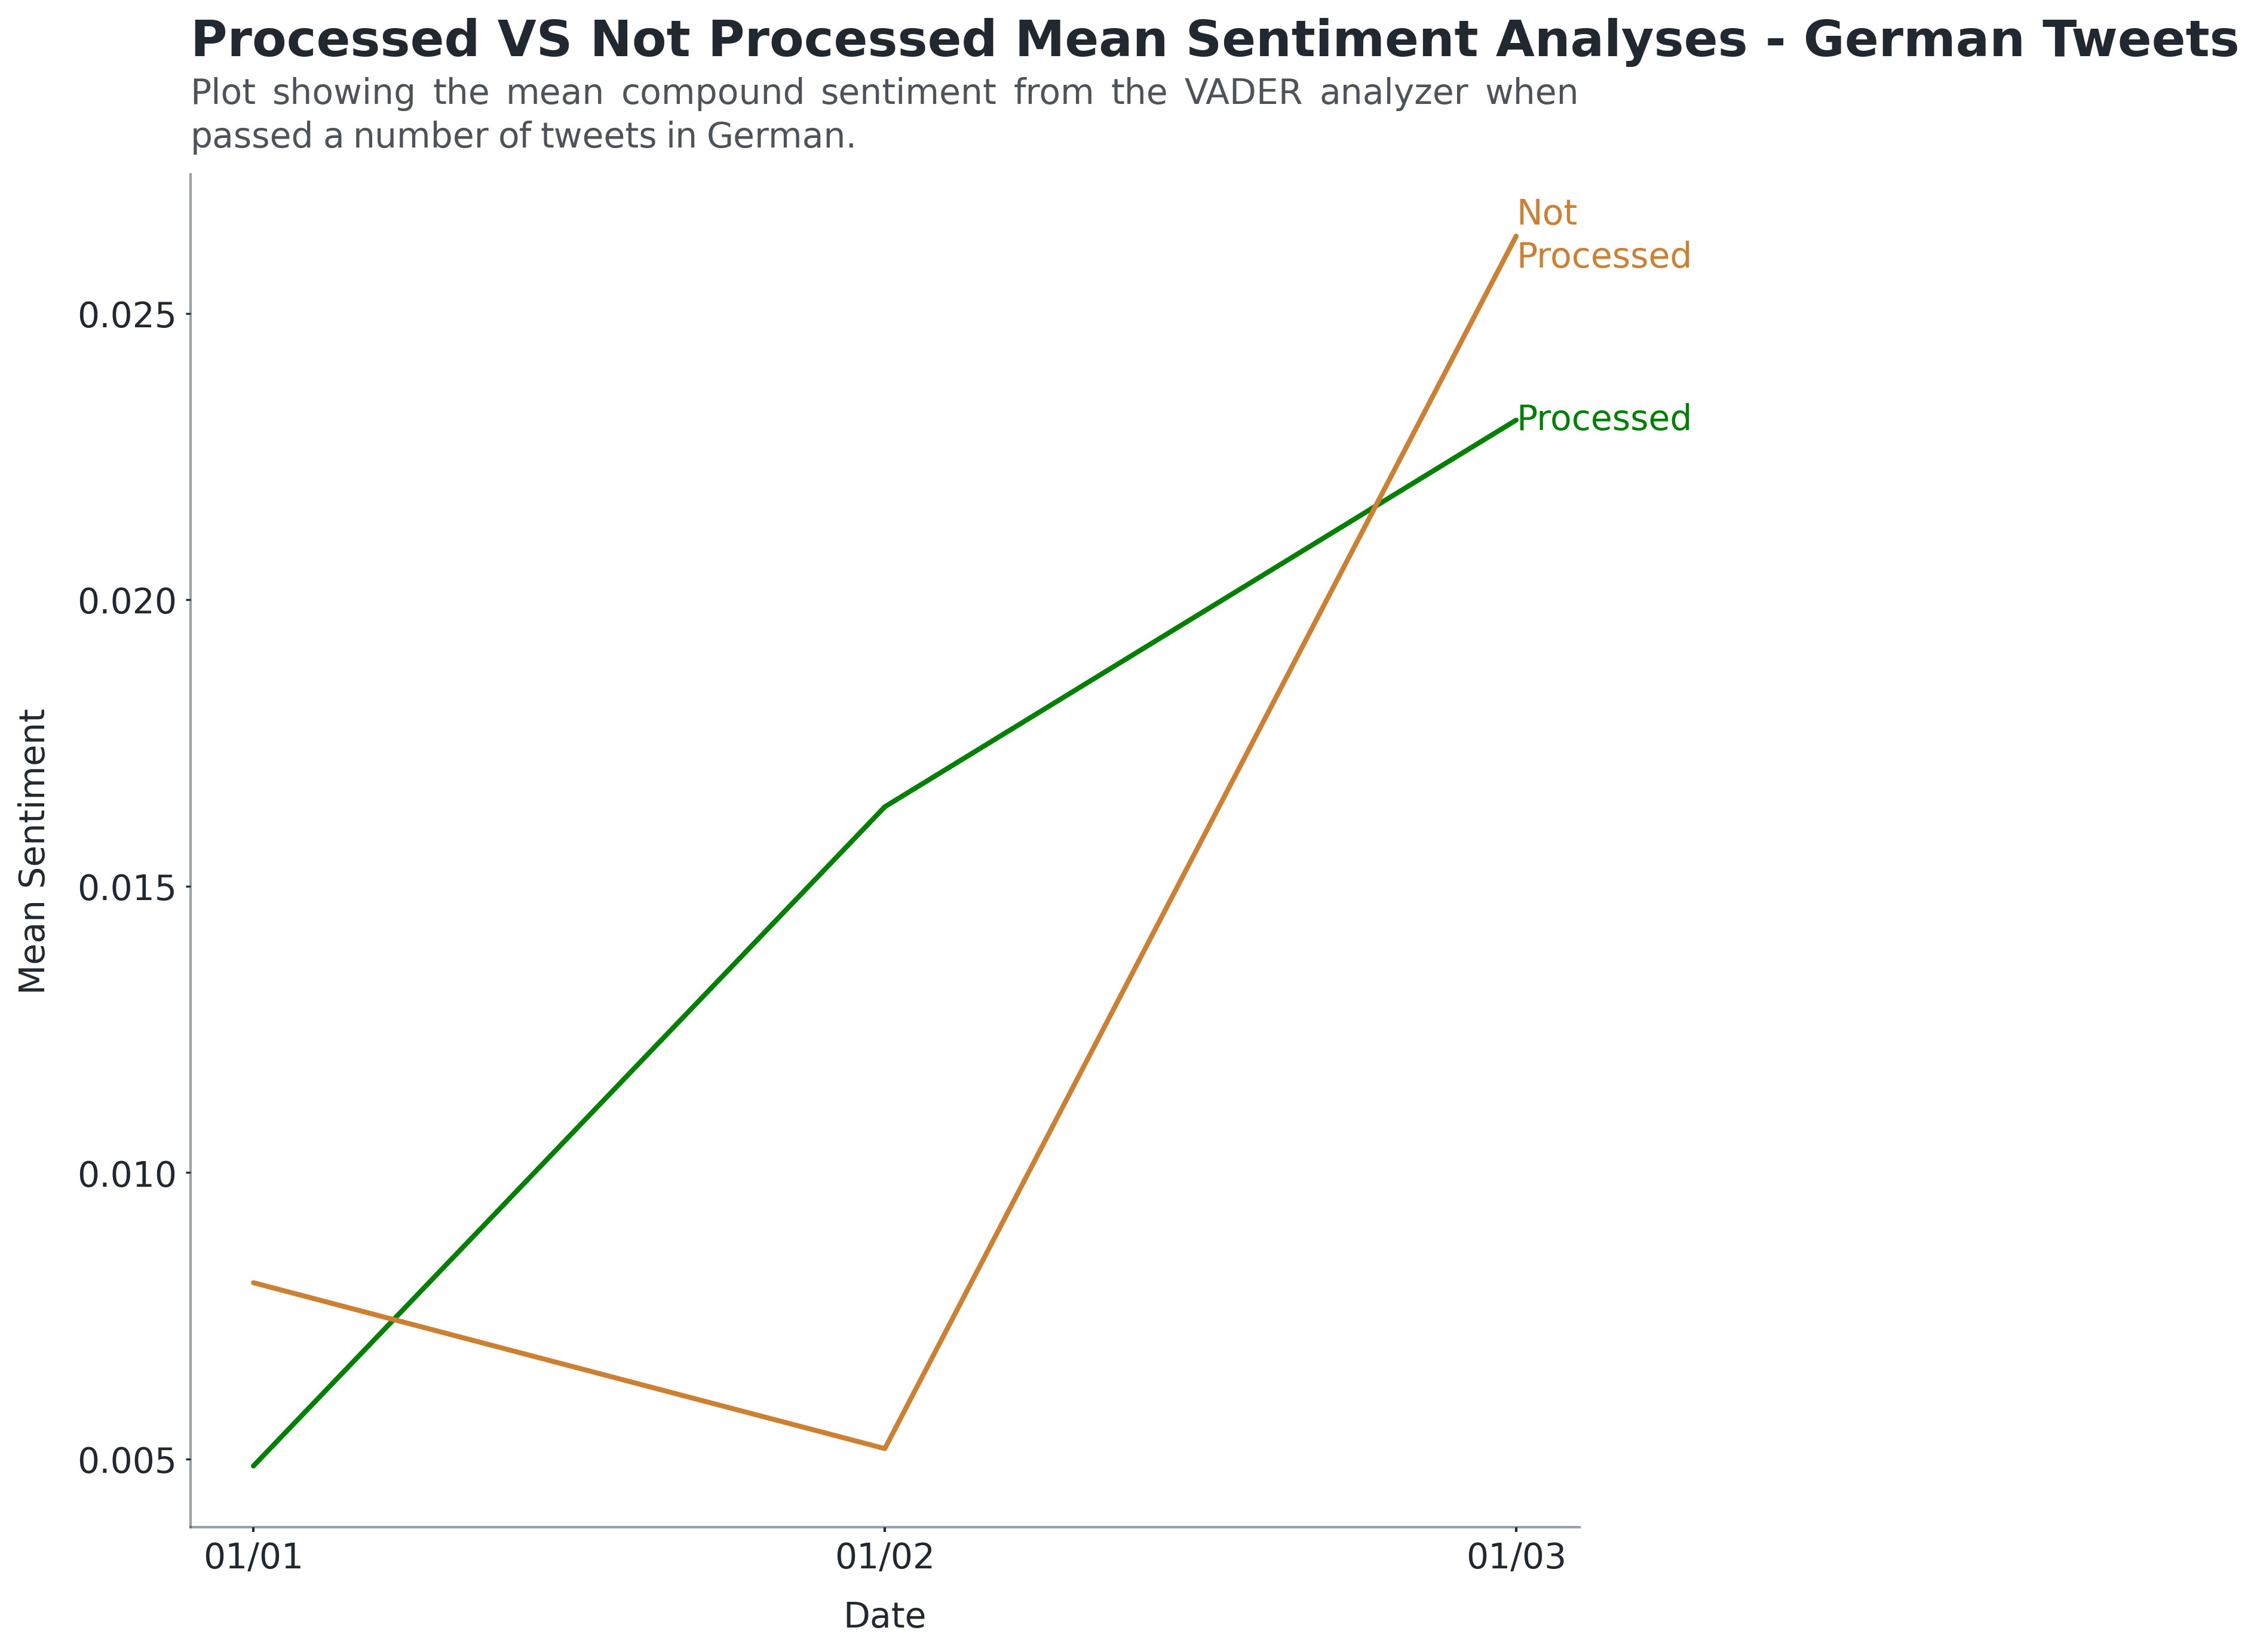
\includegraphics[width=\linewidth]{German Process VS NotProcessed.png}
  \caption[German Process VS NotProcessed]{ }\label{fig:GermanPre}
\endminipage
\end{figure}

\noindent The difference calculated along with the shapes of the graphs plotted were not considered significant enough to remove pre-processing.
However the pre-process function was amended to keep more features like emojis and hashtags, which prior to this experiment where being removed.

\newpage

\section{Daily Twitter Mean Sentiment}

Time series graphs where plotted for the mean sentiment scores on the larger 180,000 tweet dataset.

\begin{figure}[h!]
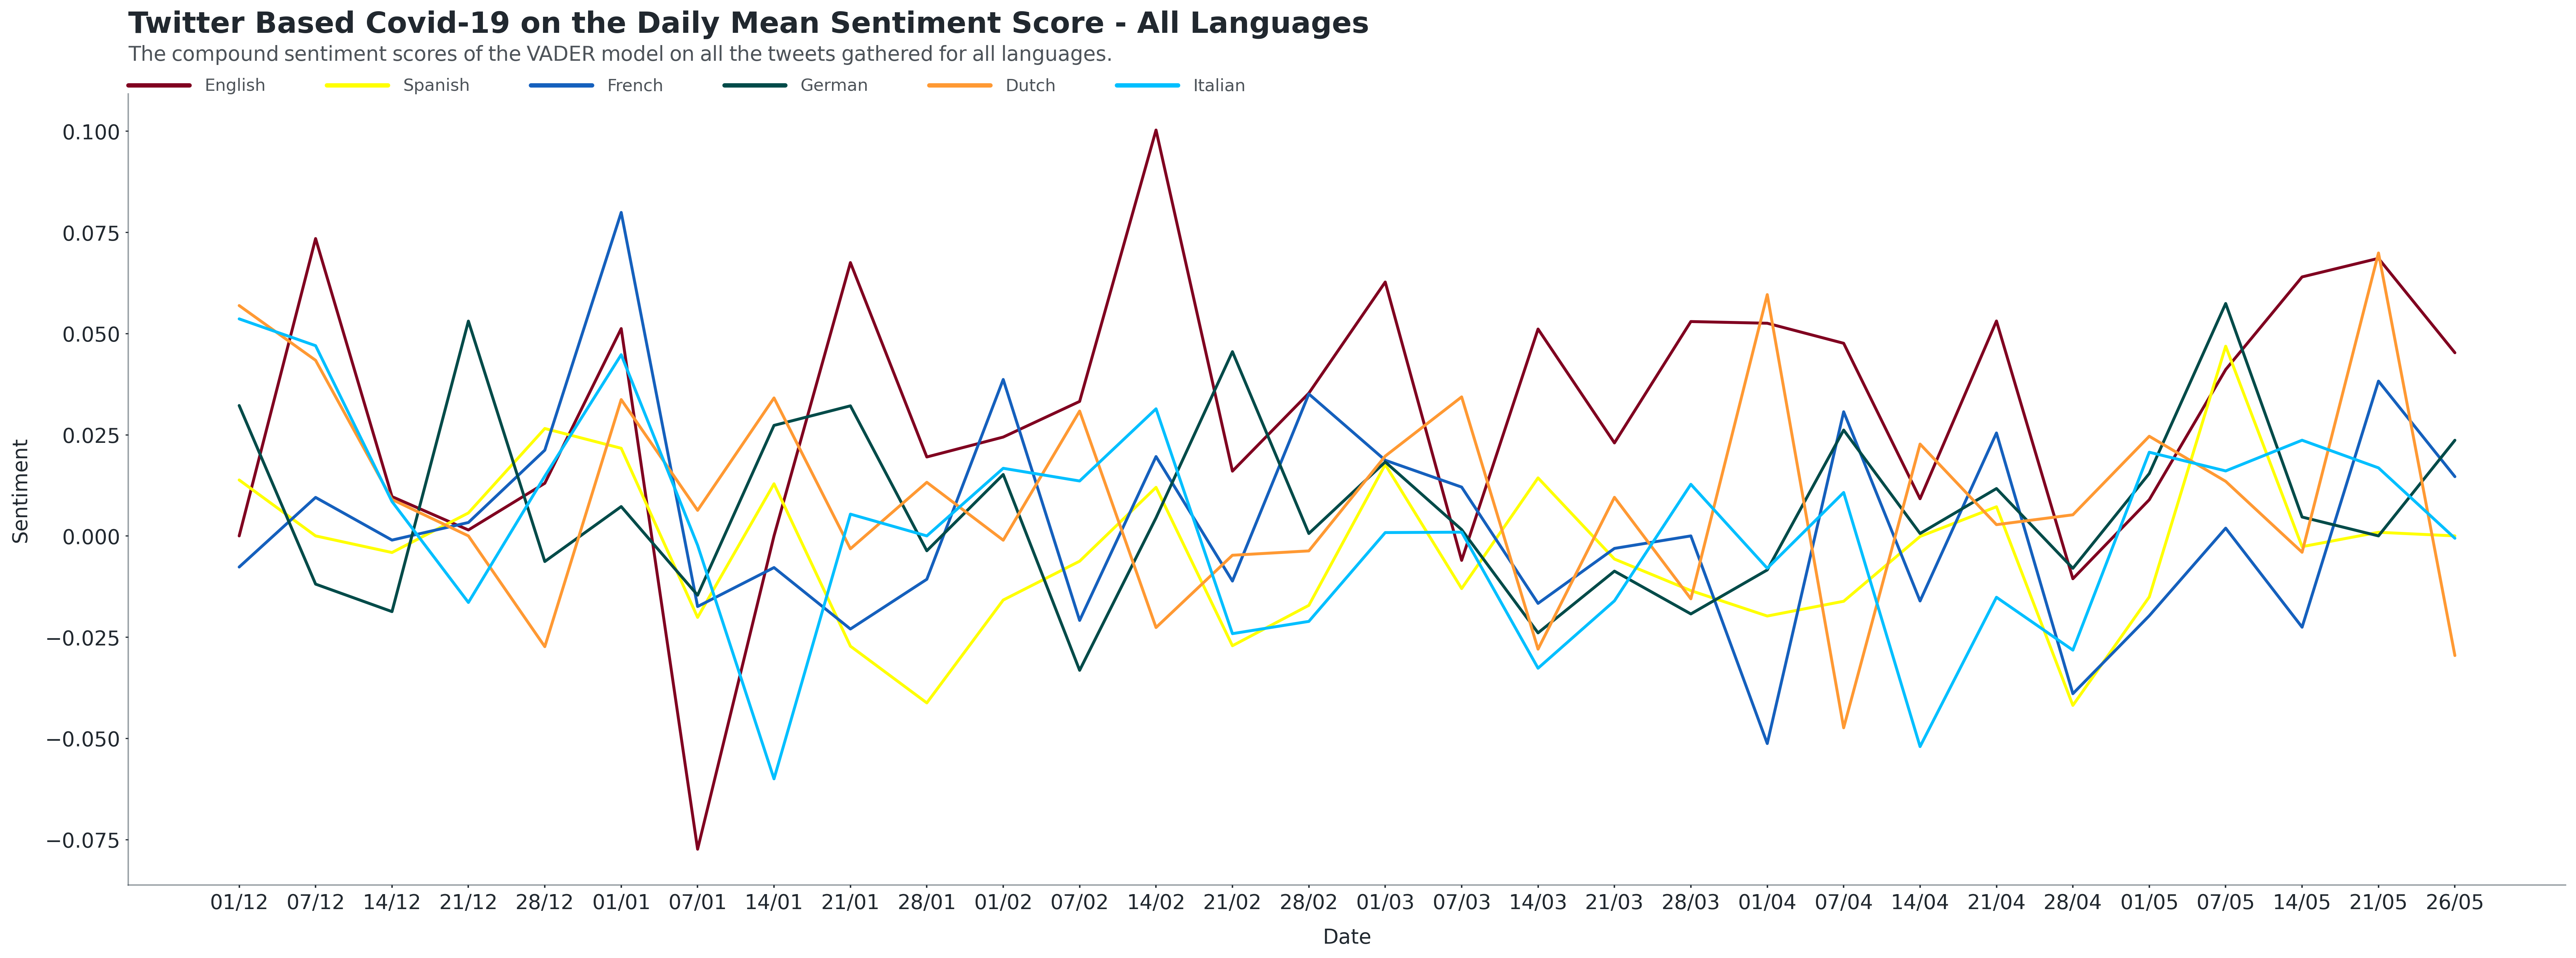
\includegraphics[scale=0.33]{Daily Mean All.png}
\caption[Daily Mean All]{ }
\label{fig:globalall}
\end{figure}


\begin{figure}[h!]
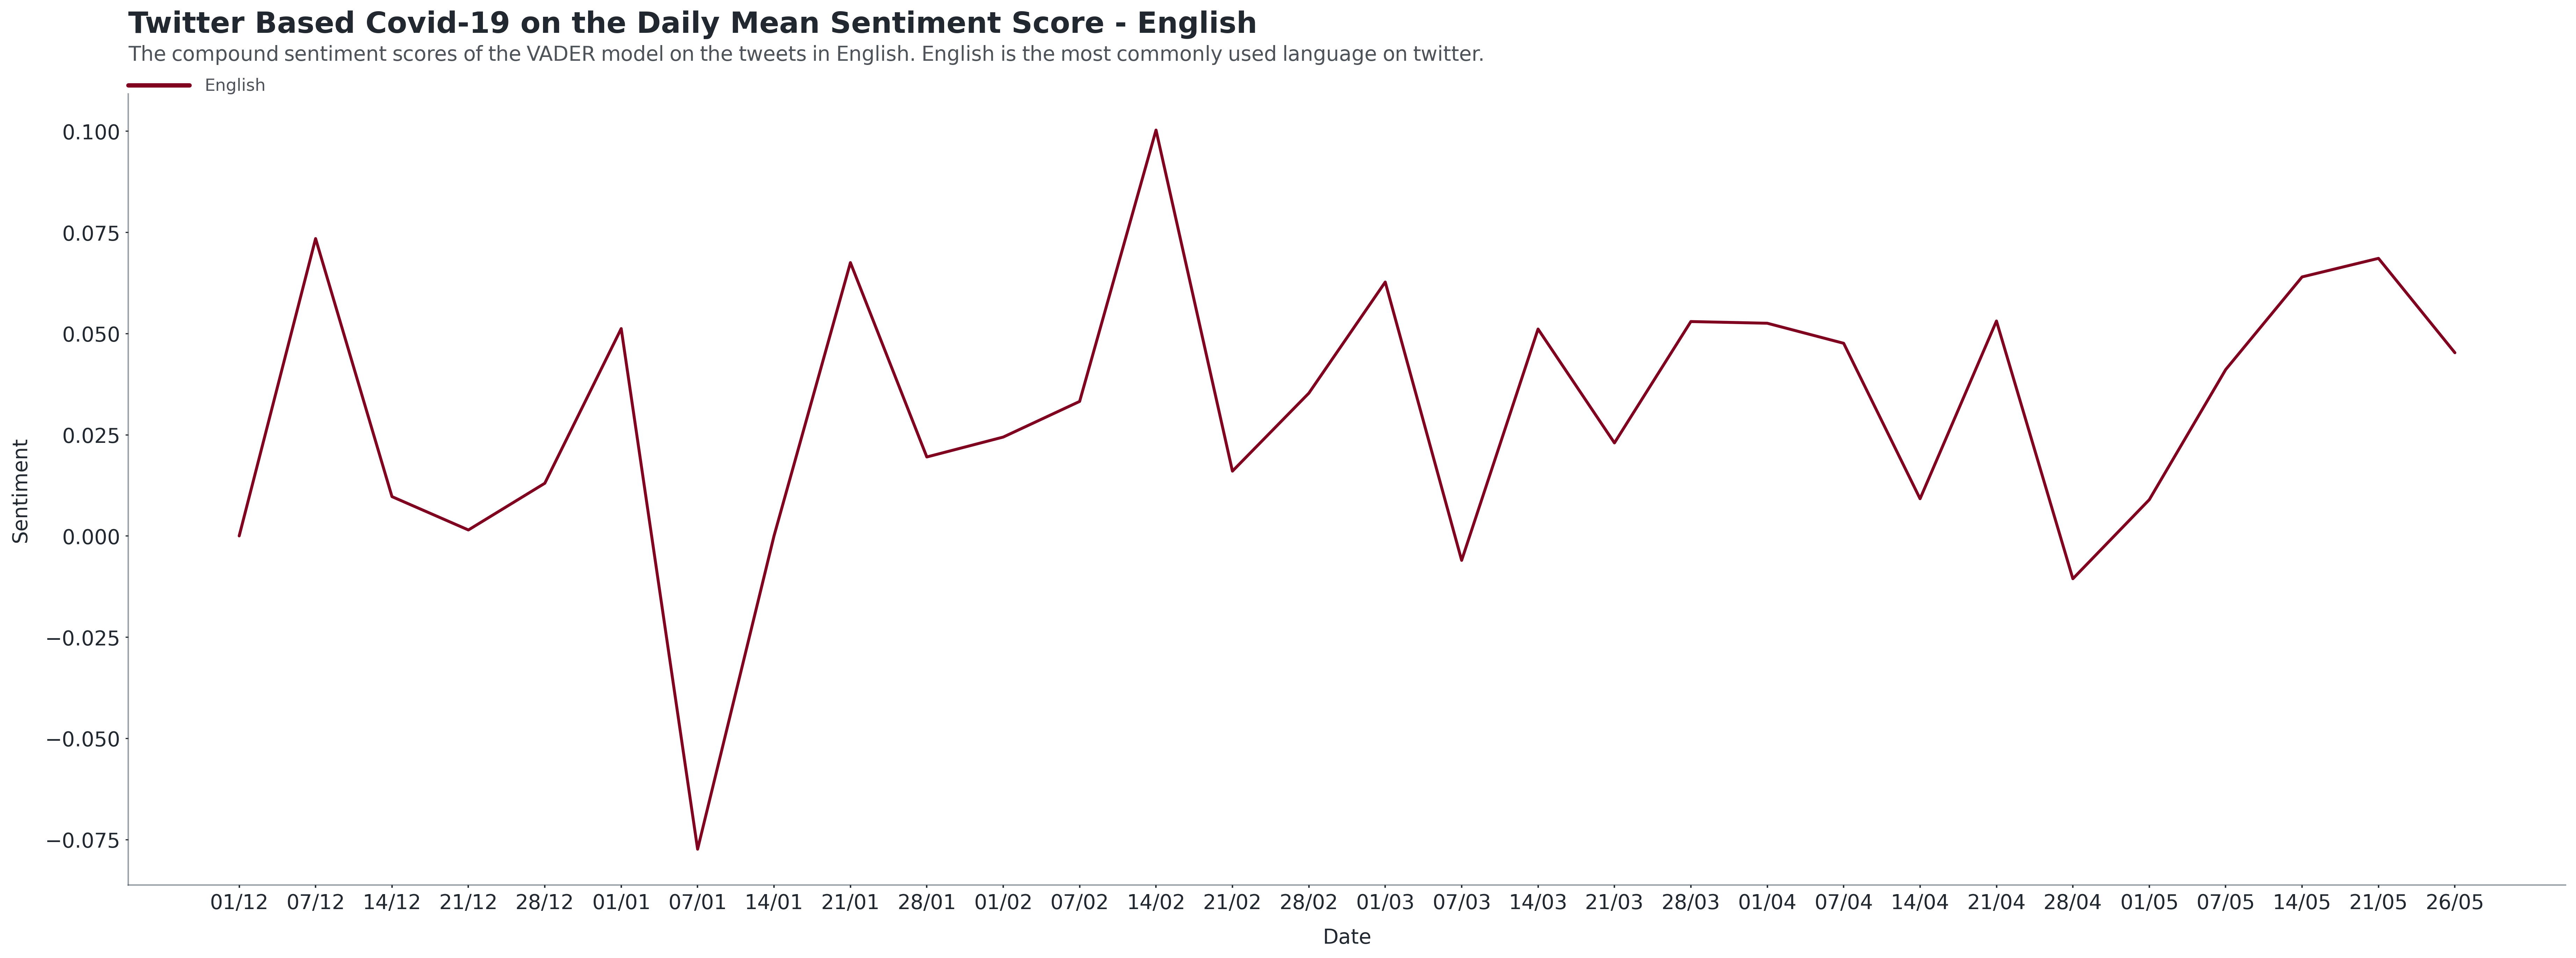
\includegraphics[scale=0.33]{Daily Mean English.png}
\caption[Daily Mean Global]{ }
\label{fig:Englishmeanap}
\end{figure}


\begin{figure}[h!]
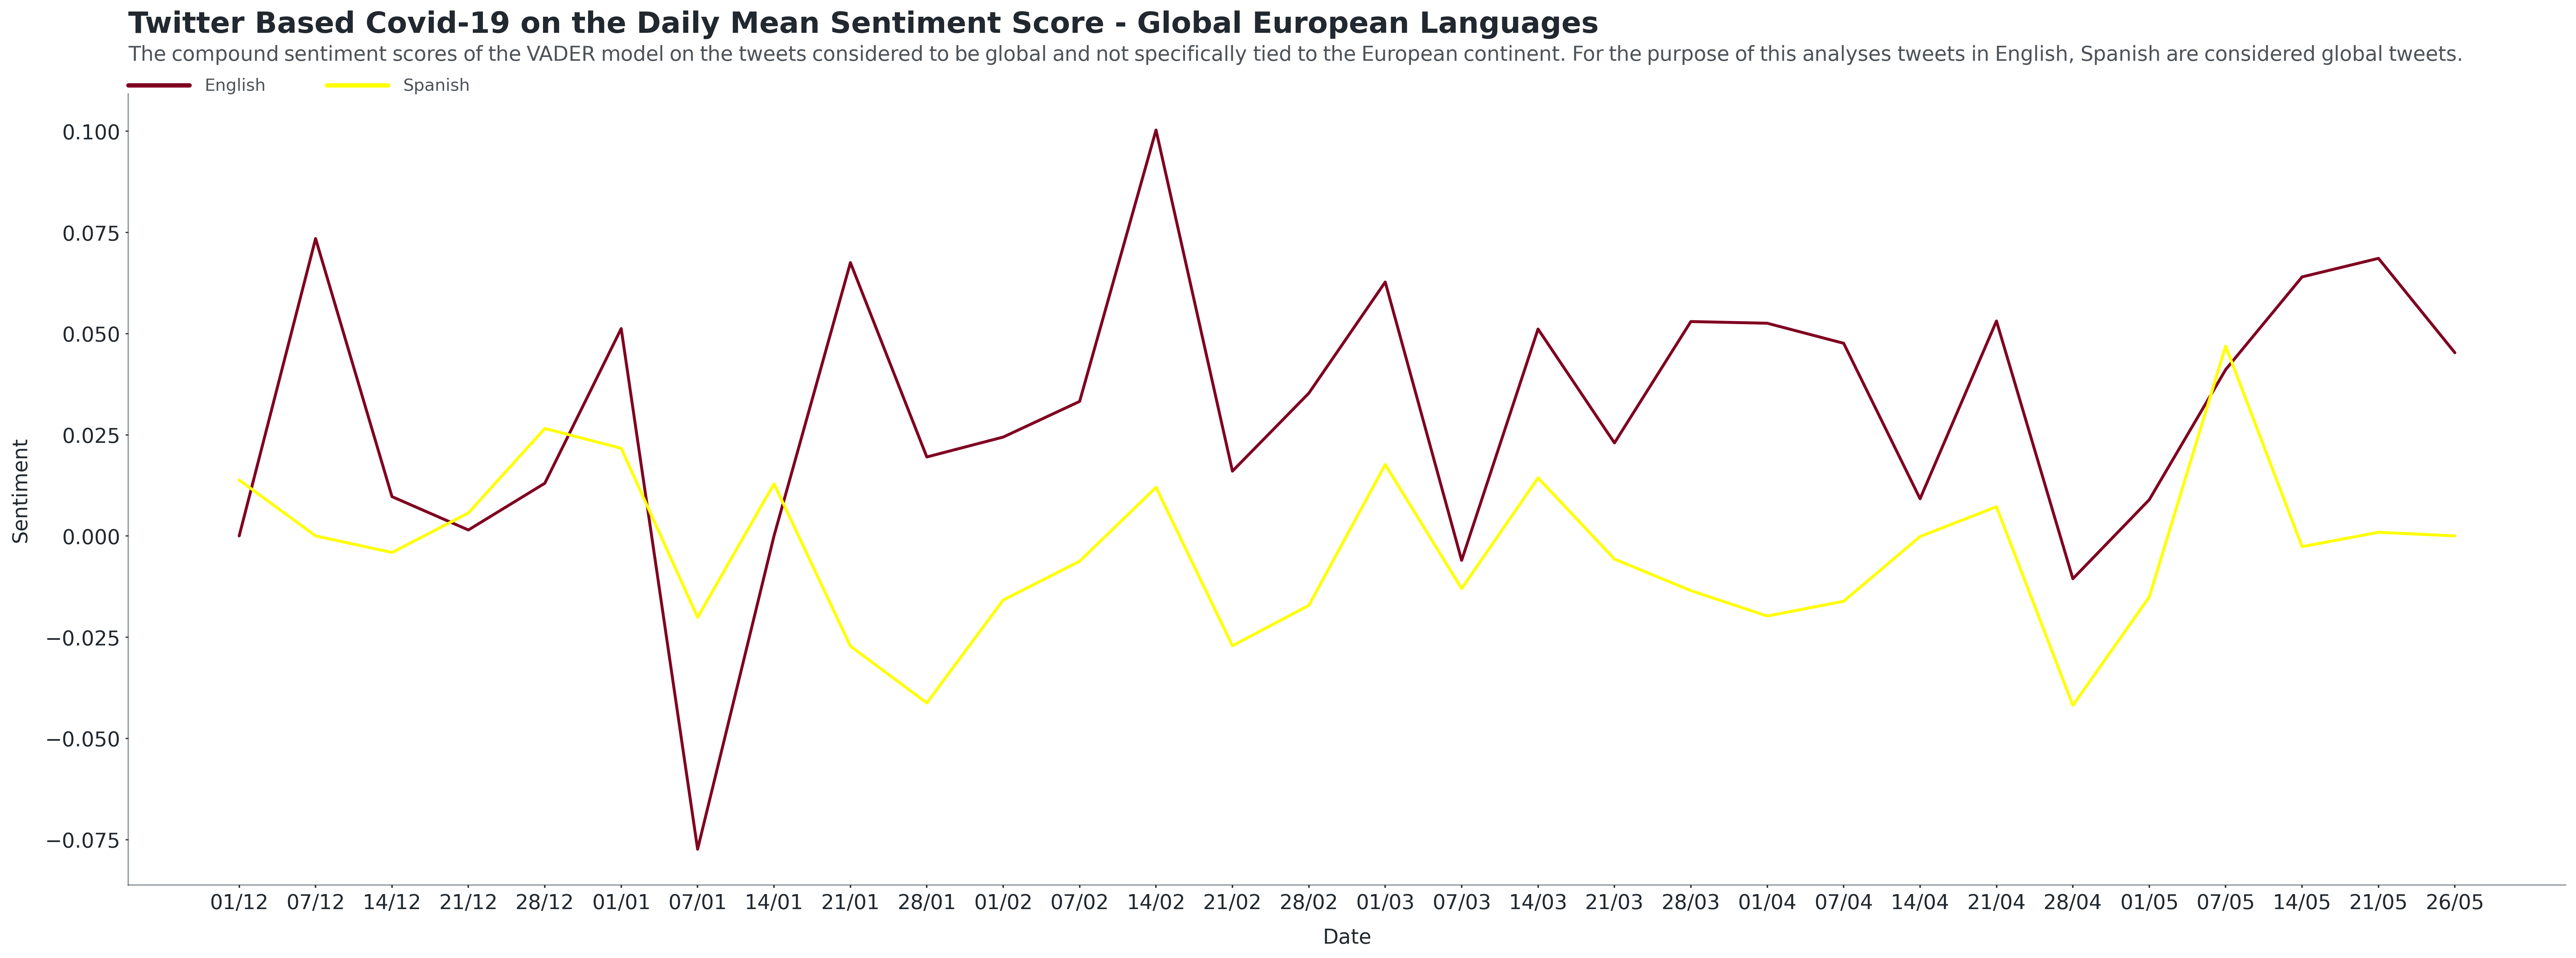
\includegraphics[scale=0.33]{Daily Mean Global.png}
\caption[Daily Mean Global]{ }
\label{fig:globalmeanap}
\end{figure}


\begin{figure}[h!]
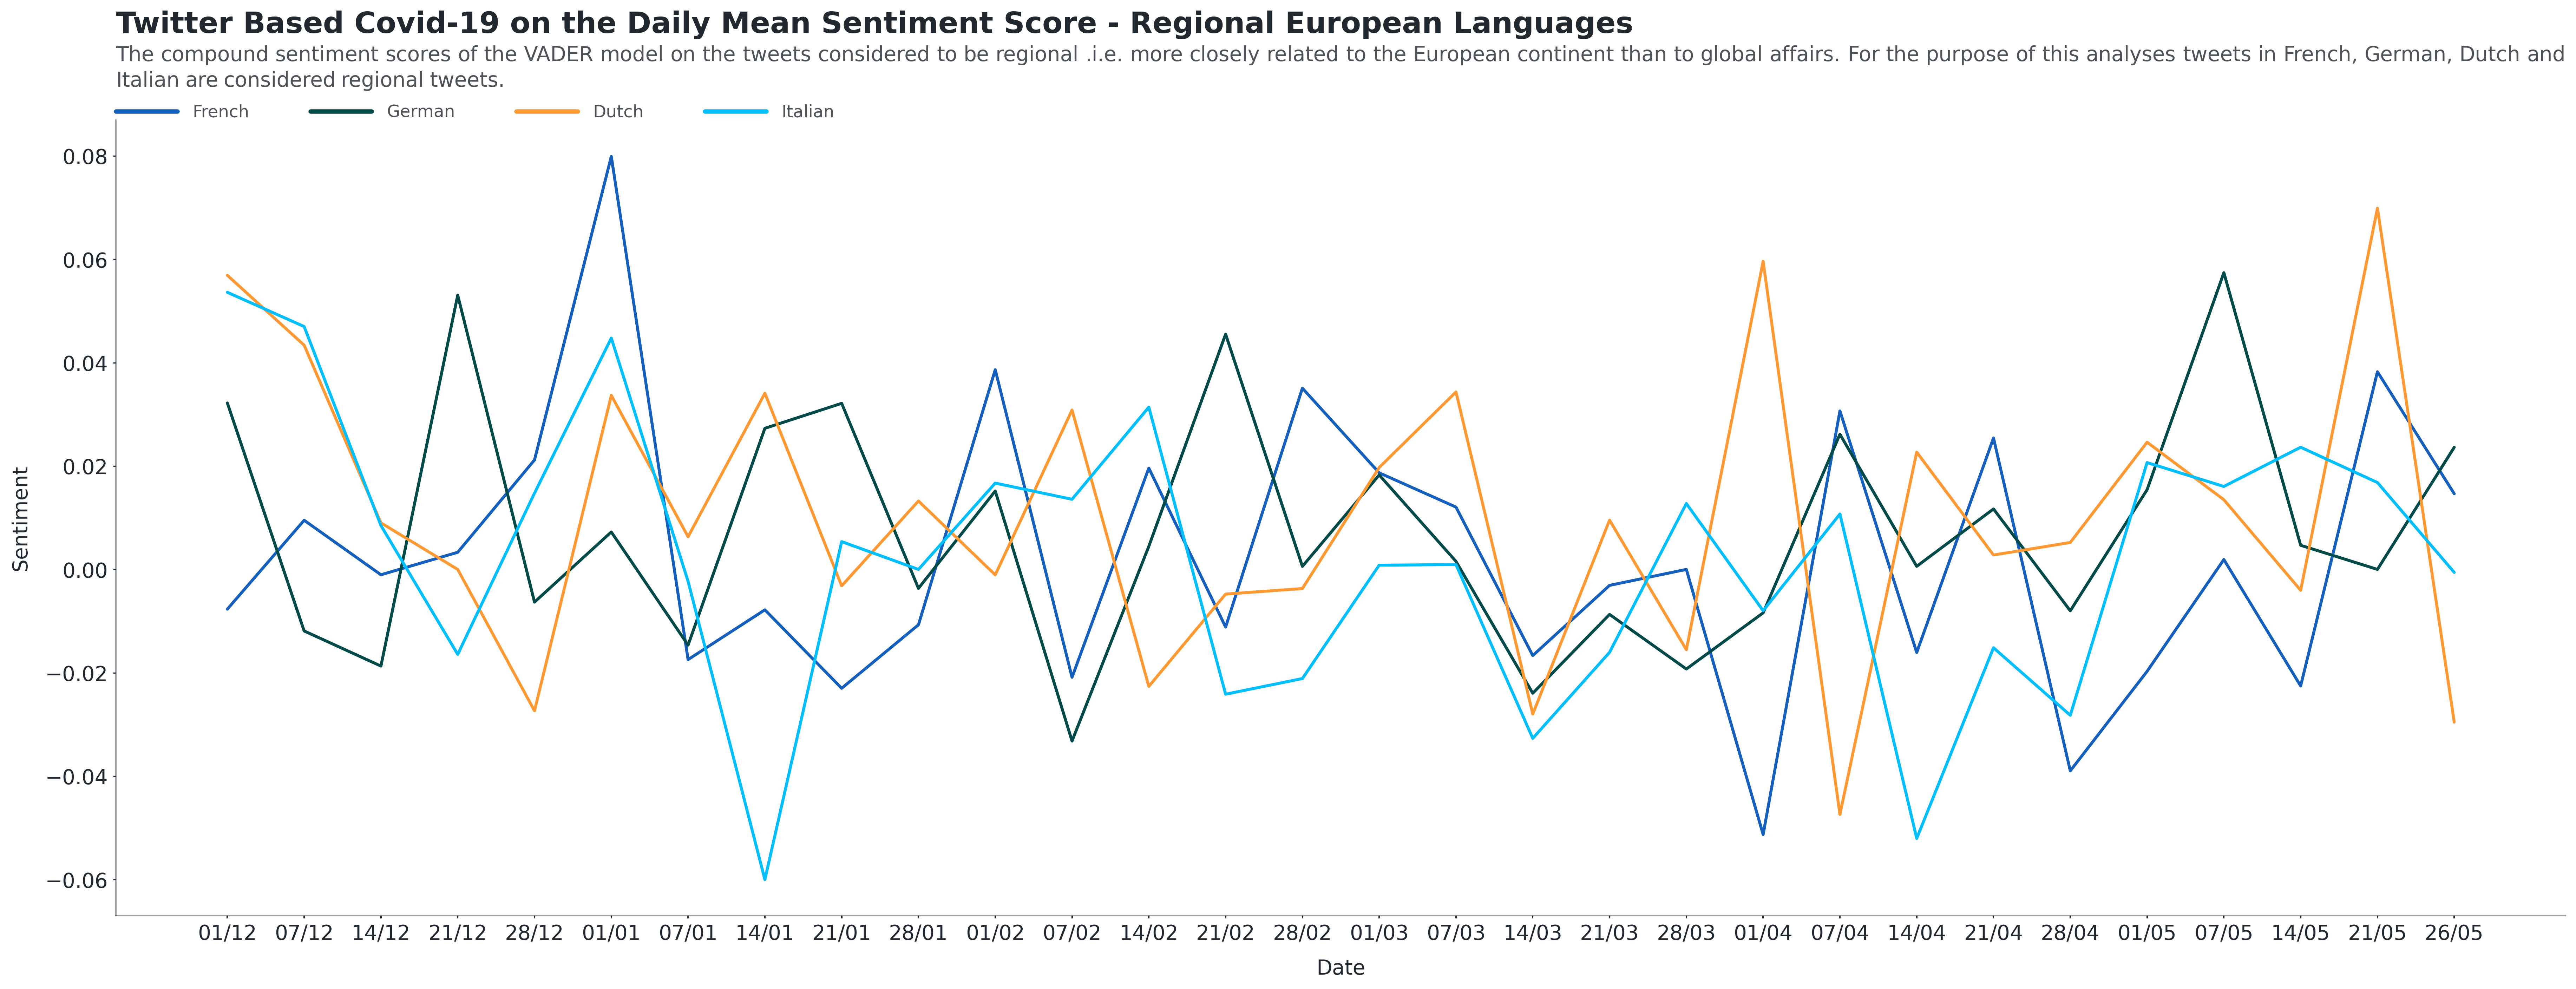
\includegraphics[scale=0.33]{Daily Mean Europe.png}
\caption[Daily Mean Europe]{ }
\label{fig:globaleu}
\end{figure}

\newpage

\section{Daily Twitter Sentiment Classification}

By classifying each compound score in a positivity class, a time series plot is plotted for each country can better visualize the changes sentiment over time.
Article headings and tweets annotated to dips and peaks of the lines in the plot to represent a random snippet of what was being said on that day.

\begin{figure}[h!]
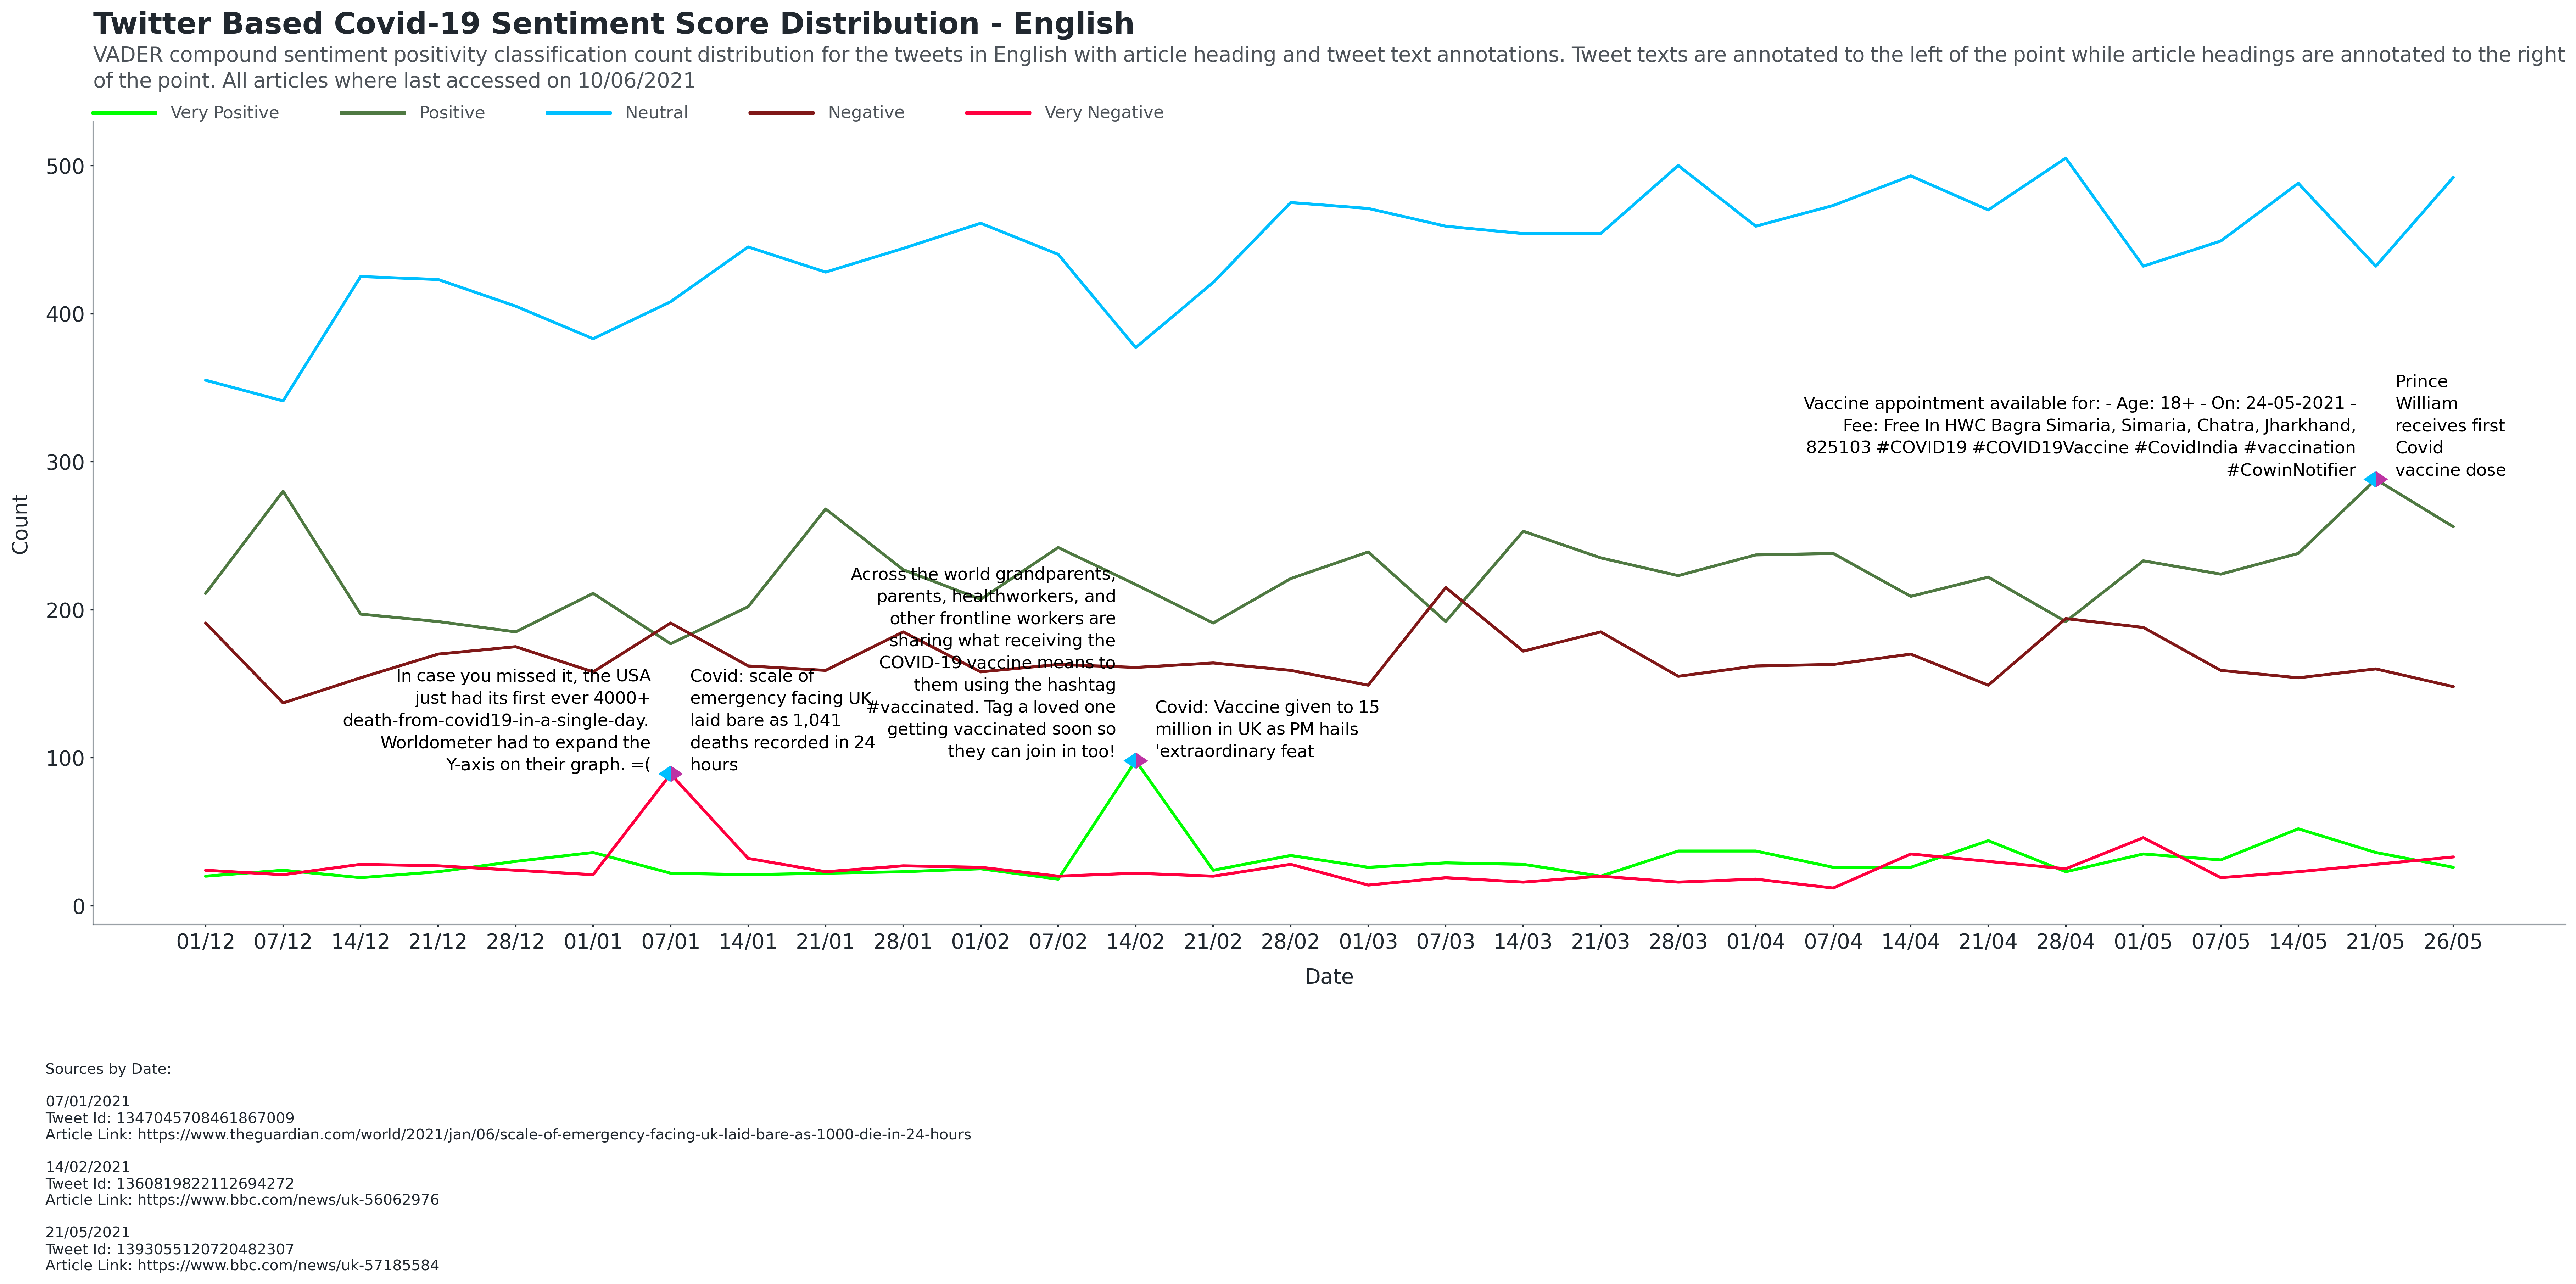
\includegraphics[scale=0.33]{Final English Annotated Distribution.png}
\caption[English Annotated Sentiment Distribution]{ }
\label{fig:English}
\end{figure}

\begin{figure}[h!]
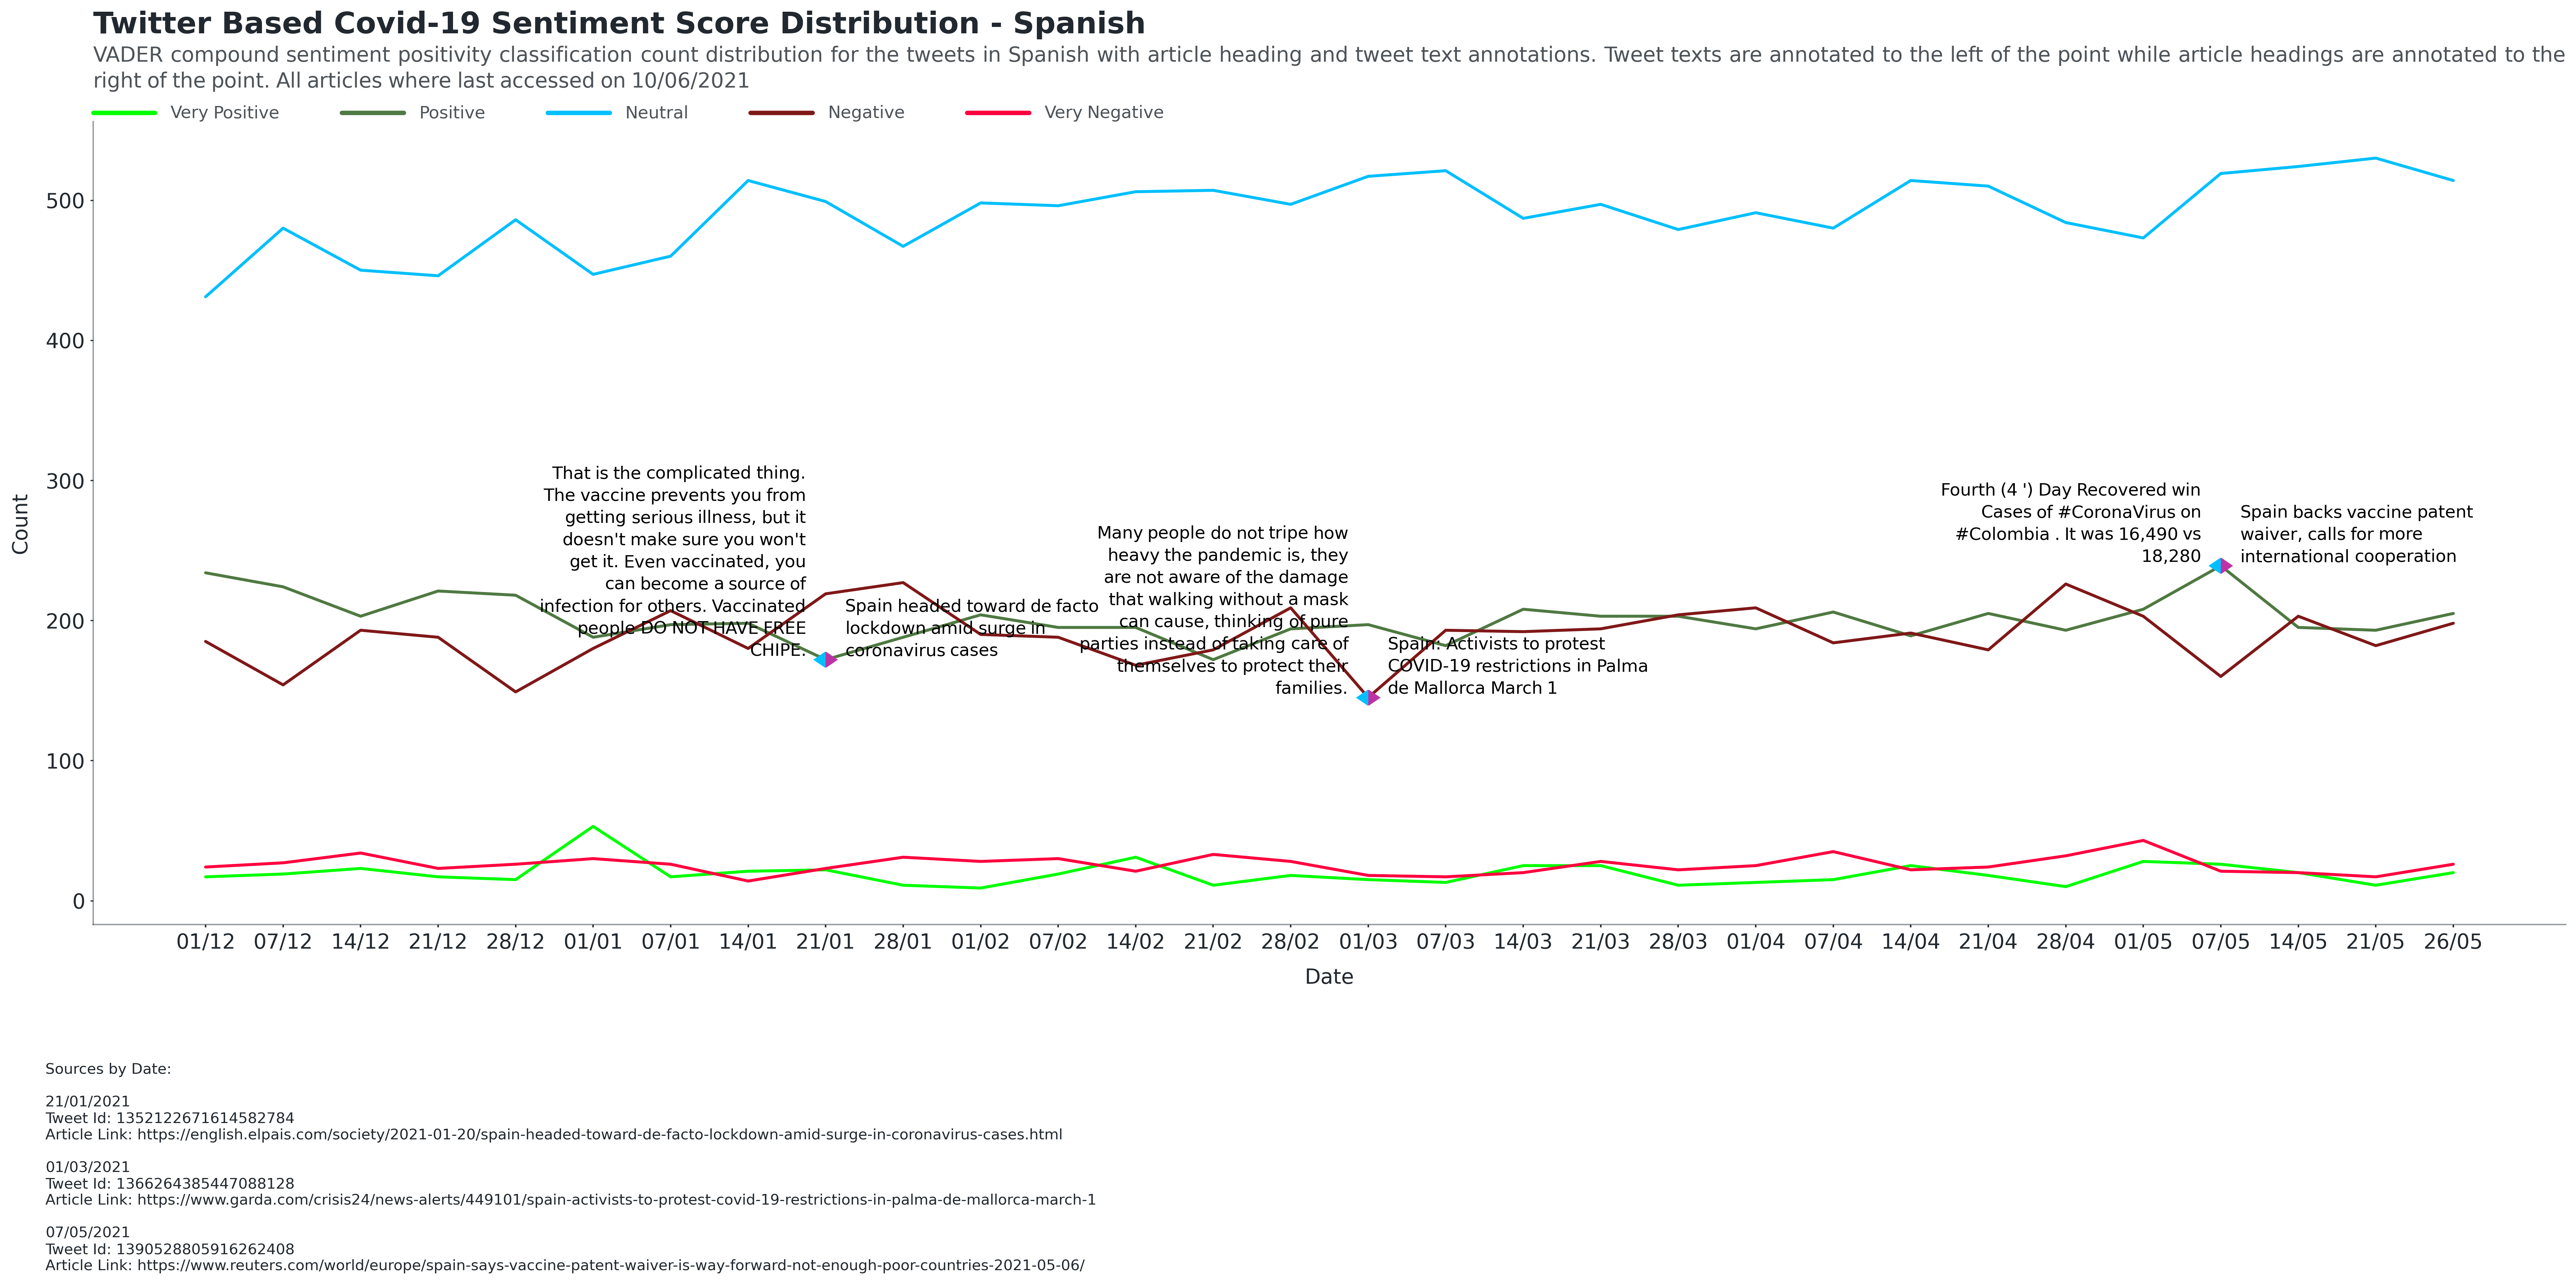
\includegraphics[scale=0.33]{Final Spanish Annotated Distribution.png}
\caption[English Annotated Sentiment Distribution]{ }
\label{fig:Spanish}
\end{figure}

\begin{figure}[h!]
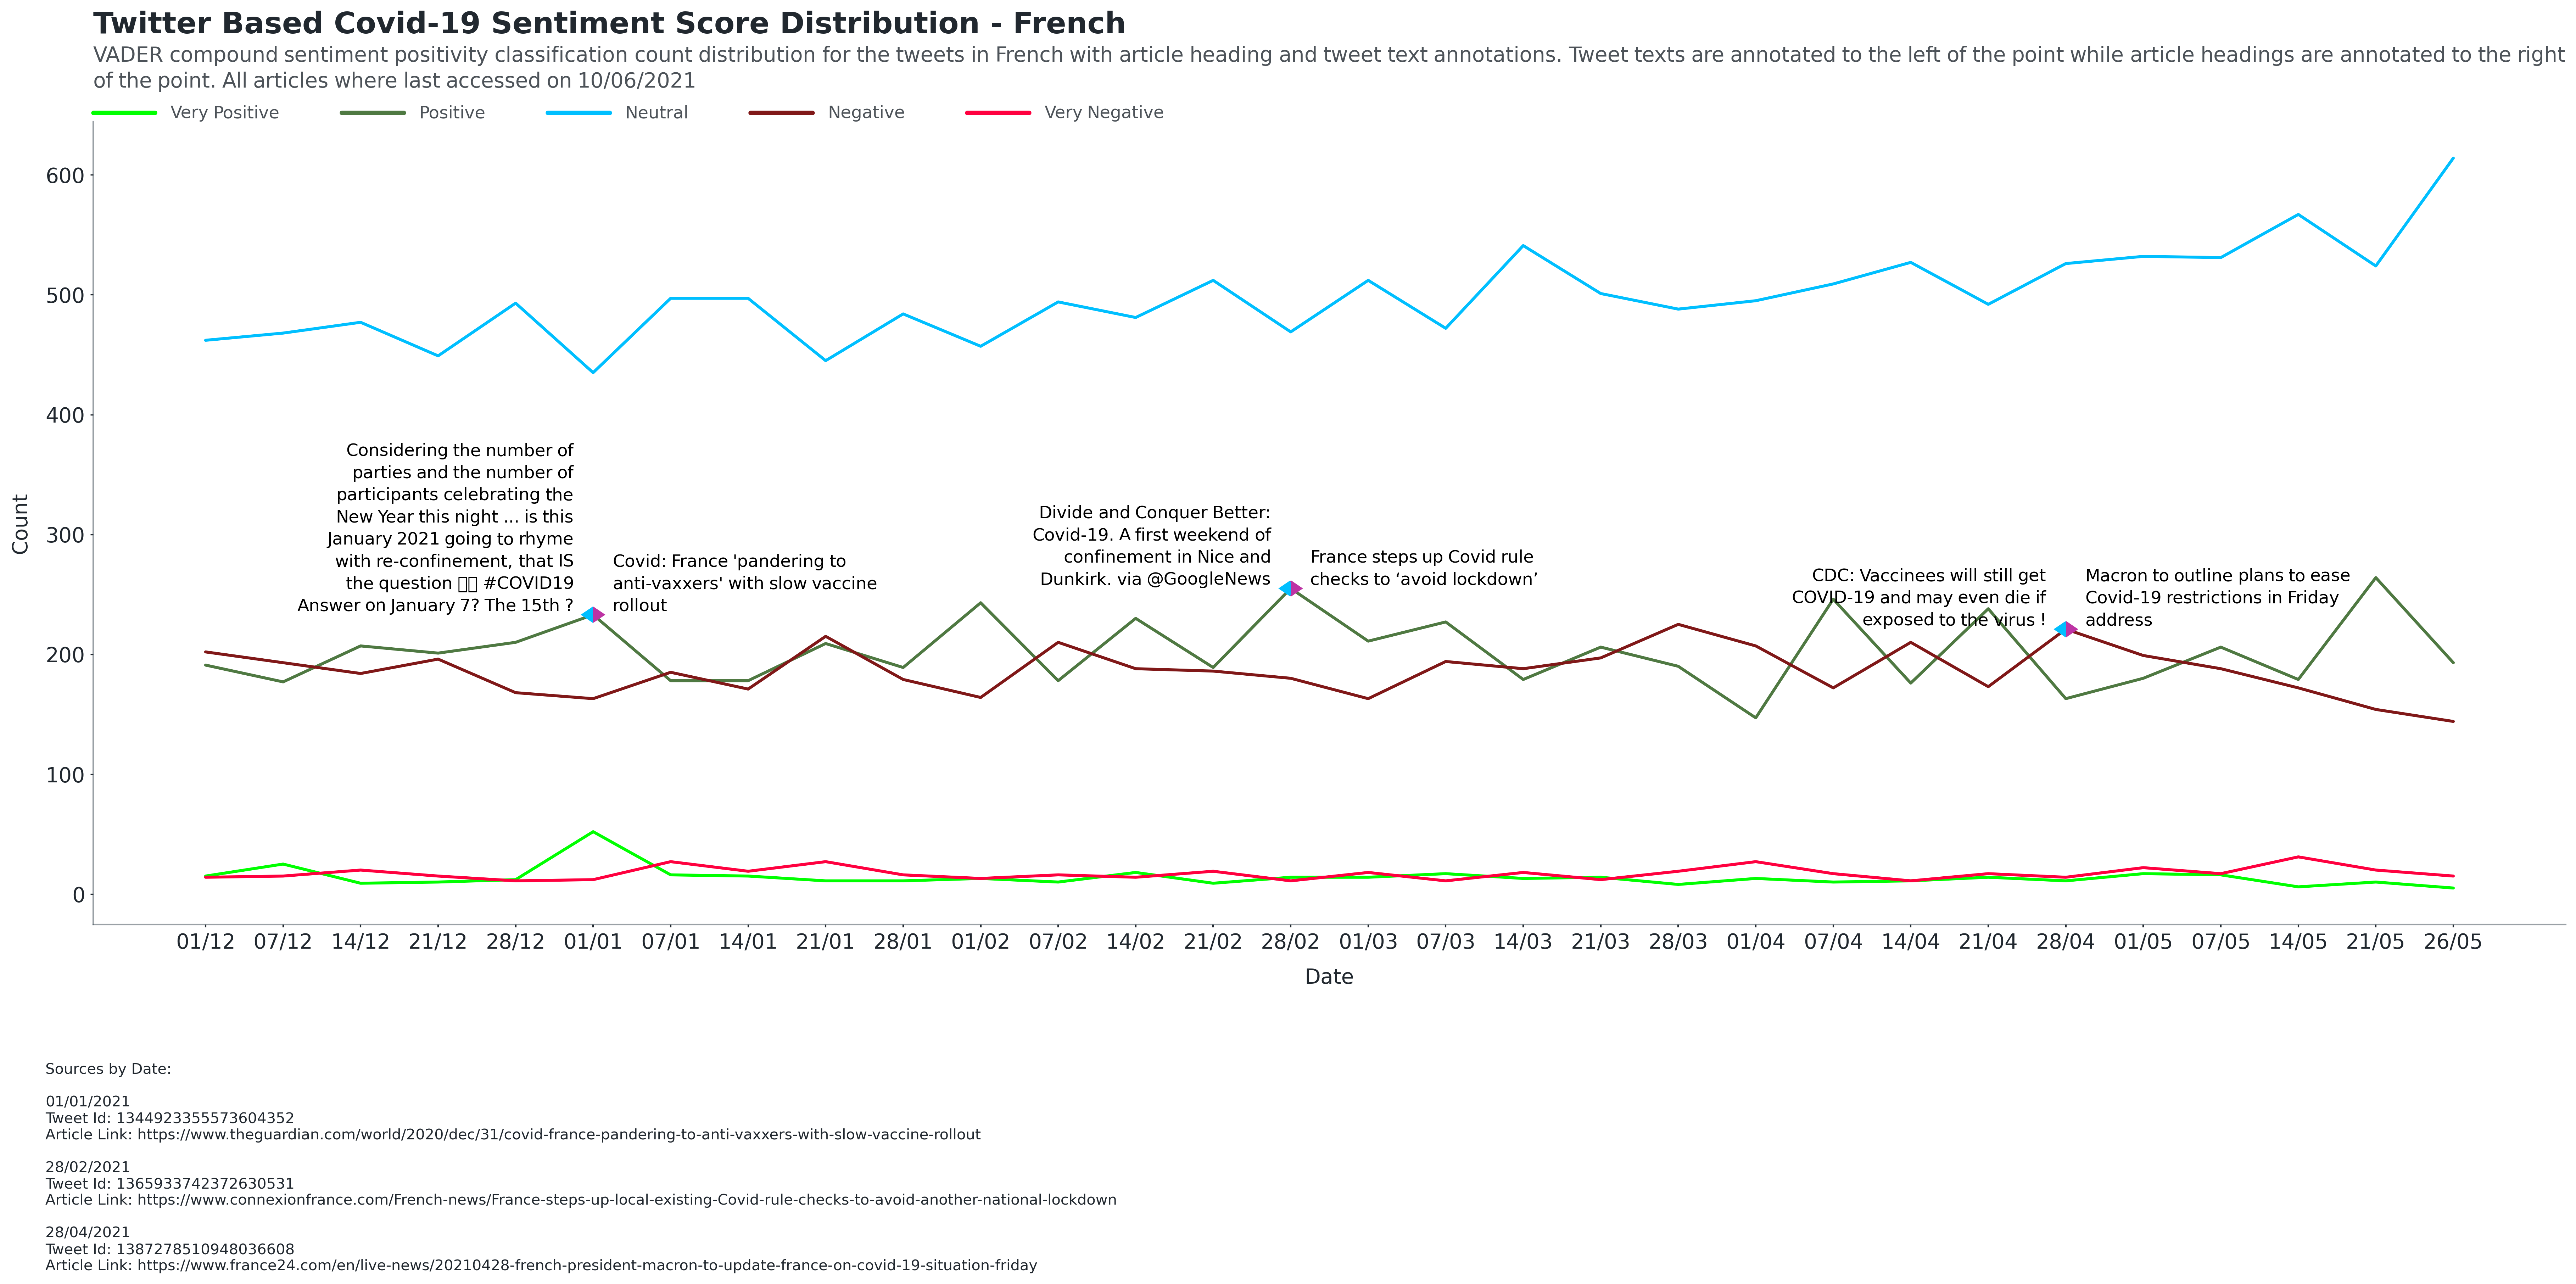
\includegraphics[scale=0.33]{Final French Annotated Distribution.png}
\caption[Final French Annotated Distribution]{ }
\label{fig:French}
\end{figure}

\begin{figure}[h!]
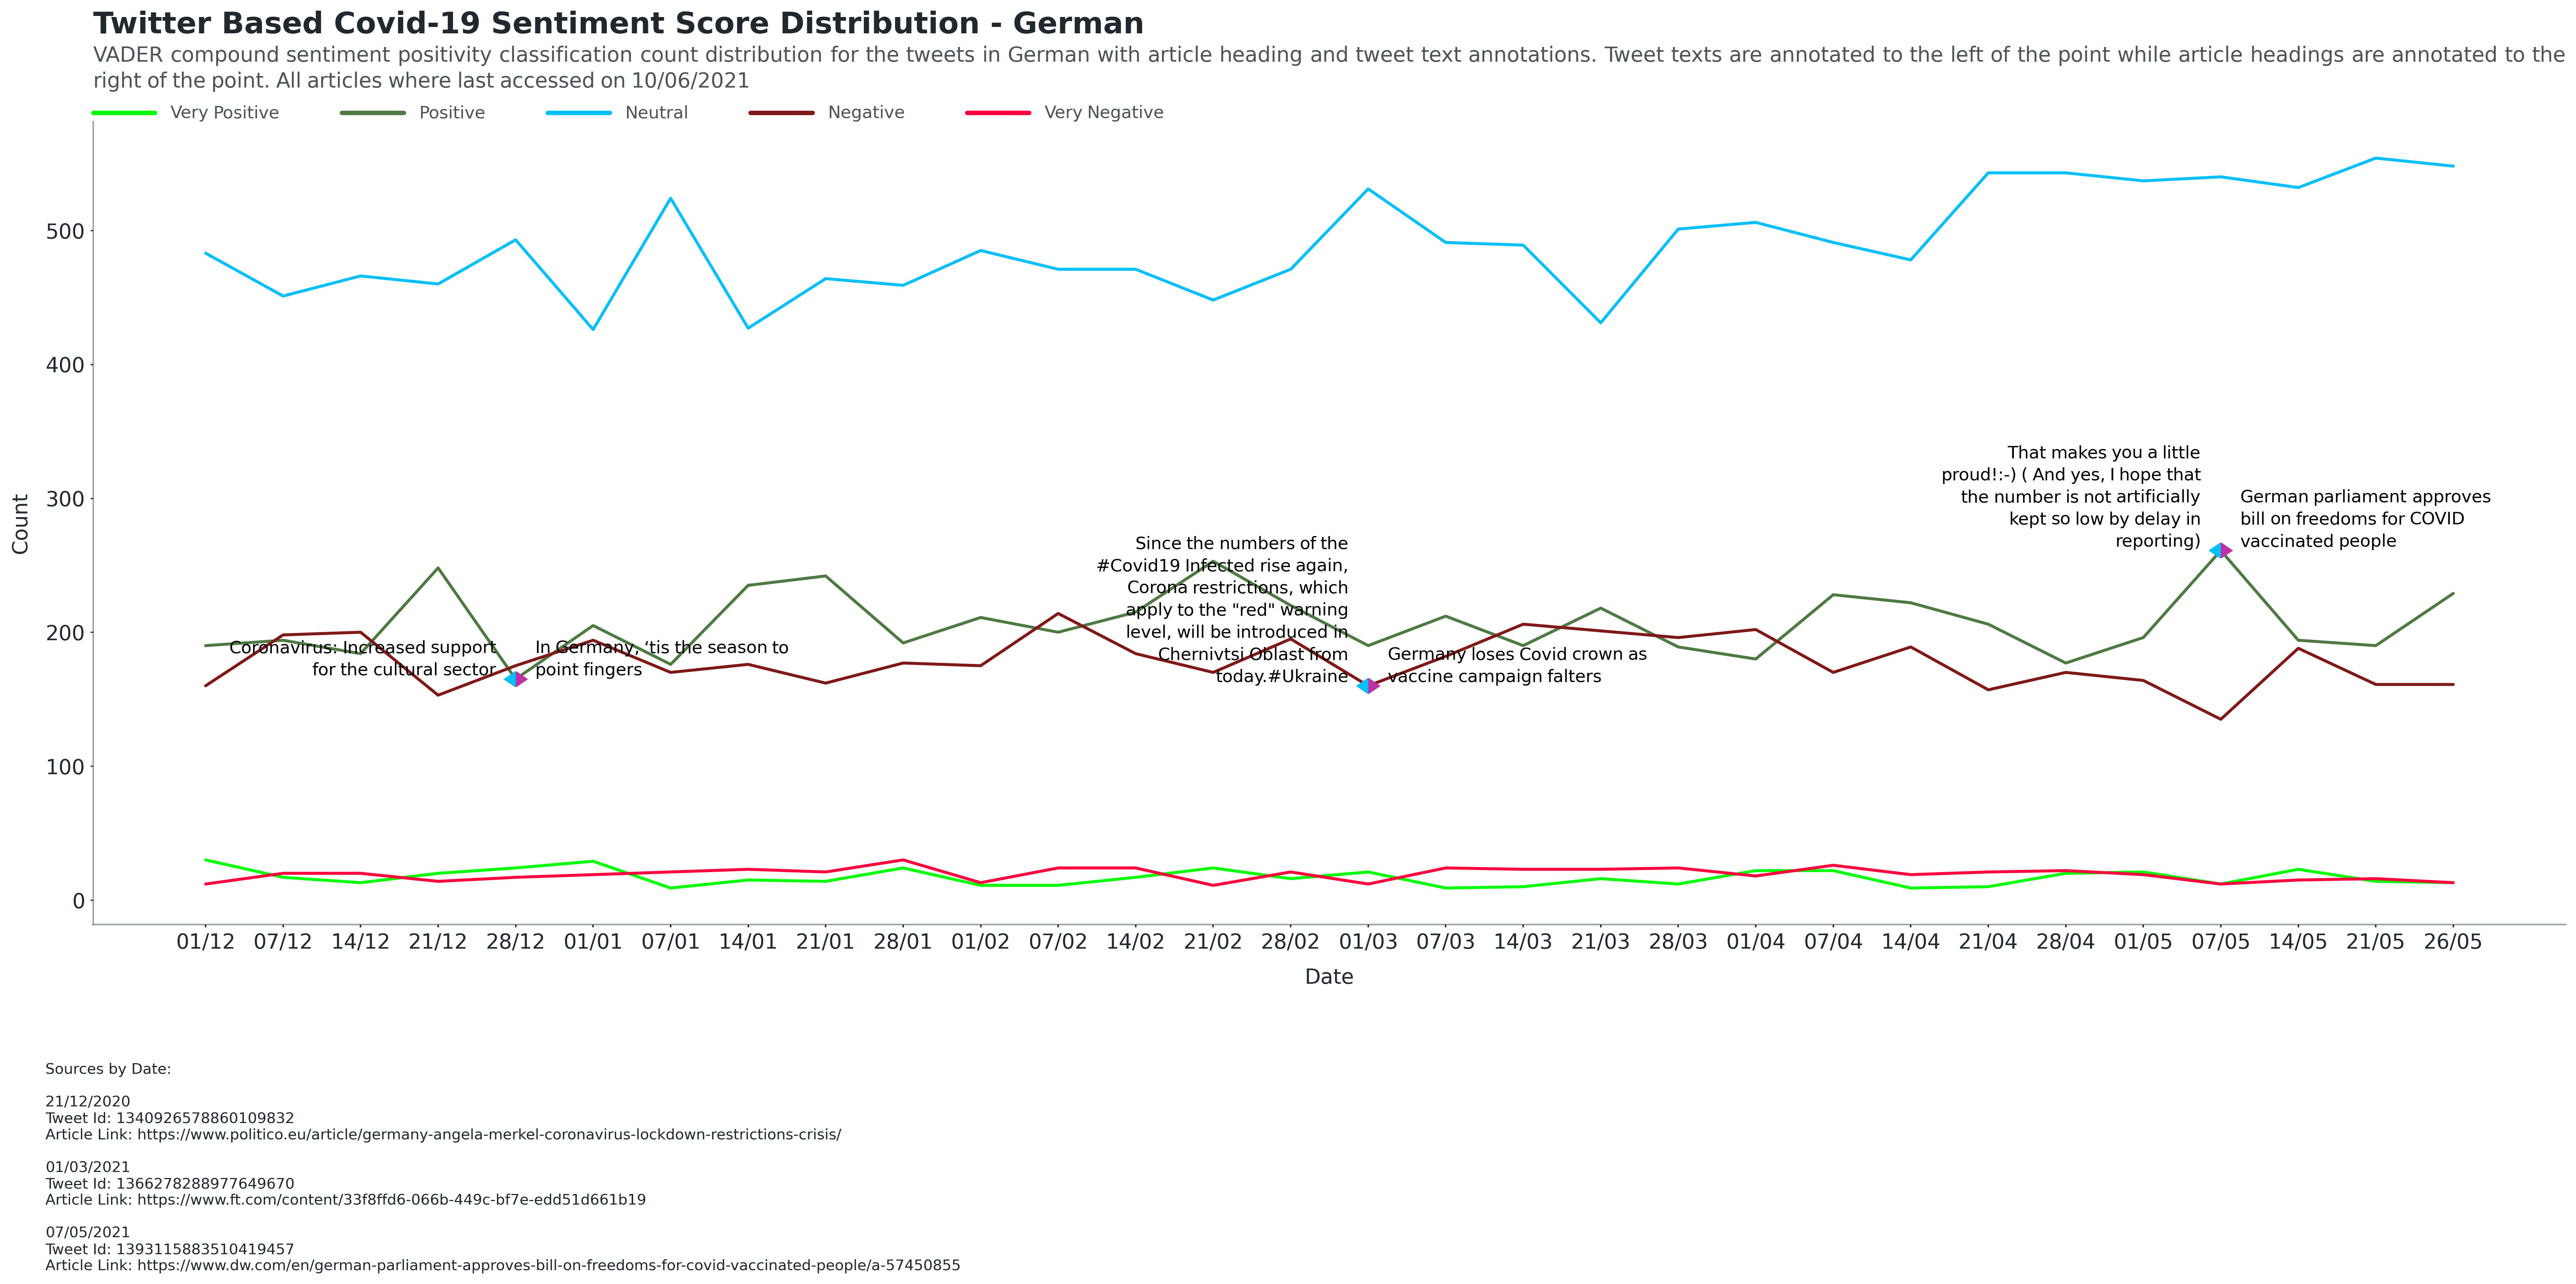
\includegraphics[scale=0.33]{Final German Annotated Distribution.png}
\caption[Final German Annotated Distribution]{ }
\label{fig:German}
\end{figure}

\begin{figure}[h!]
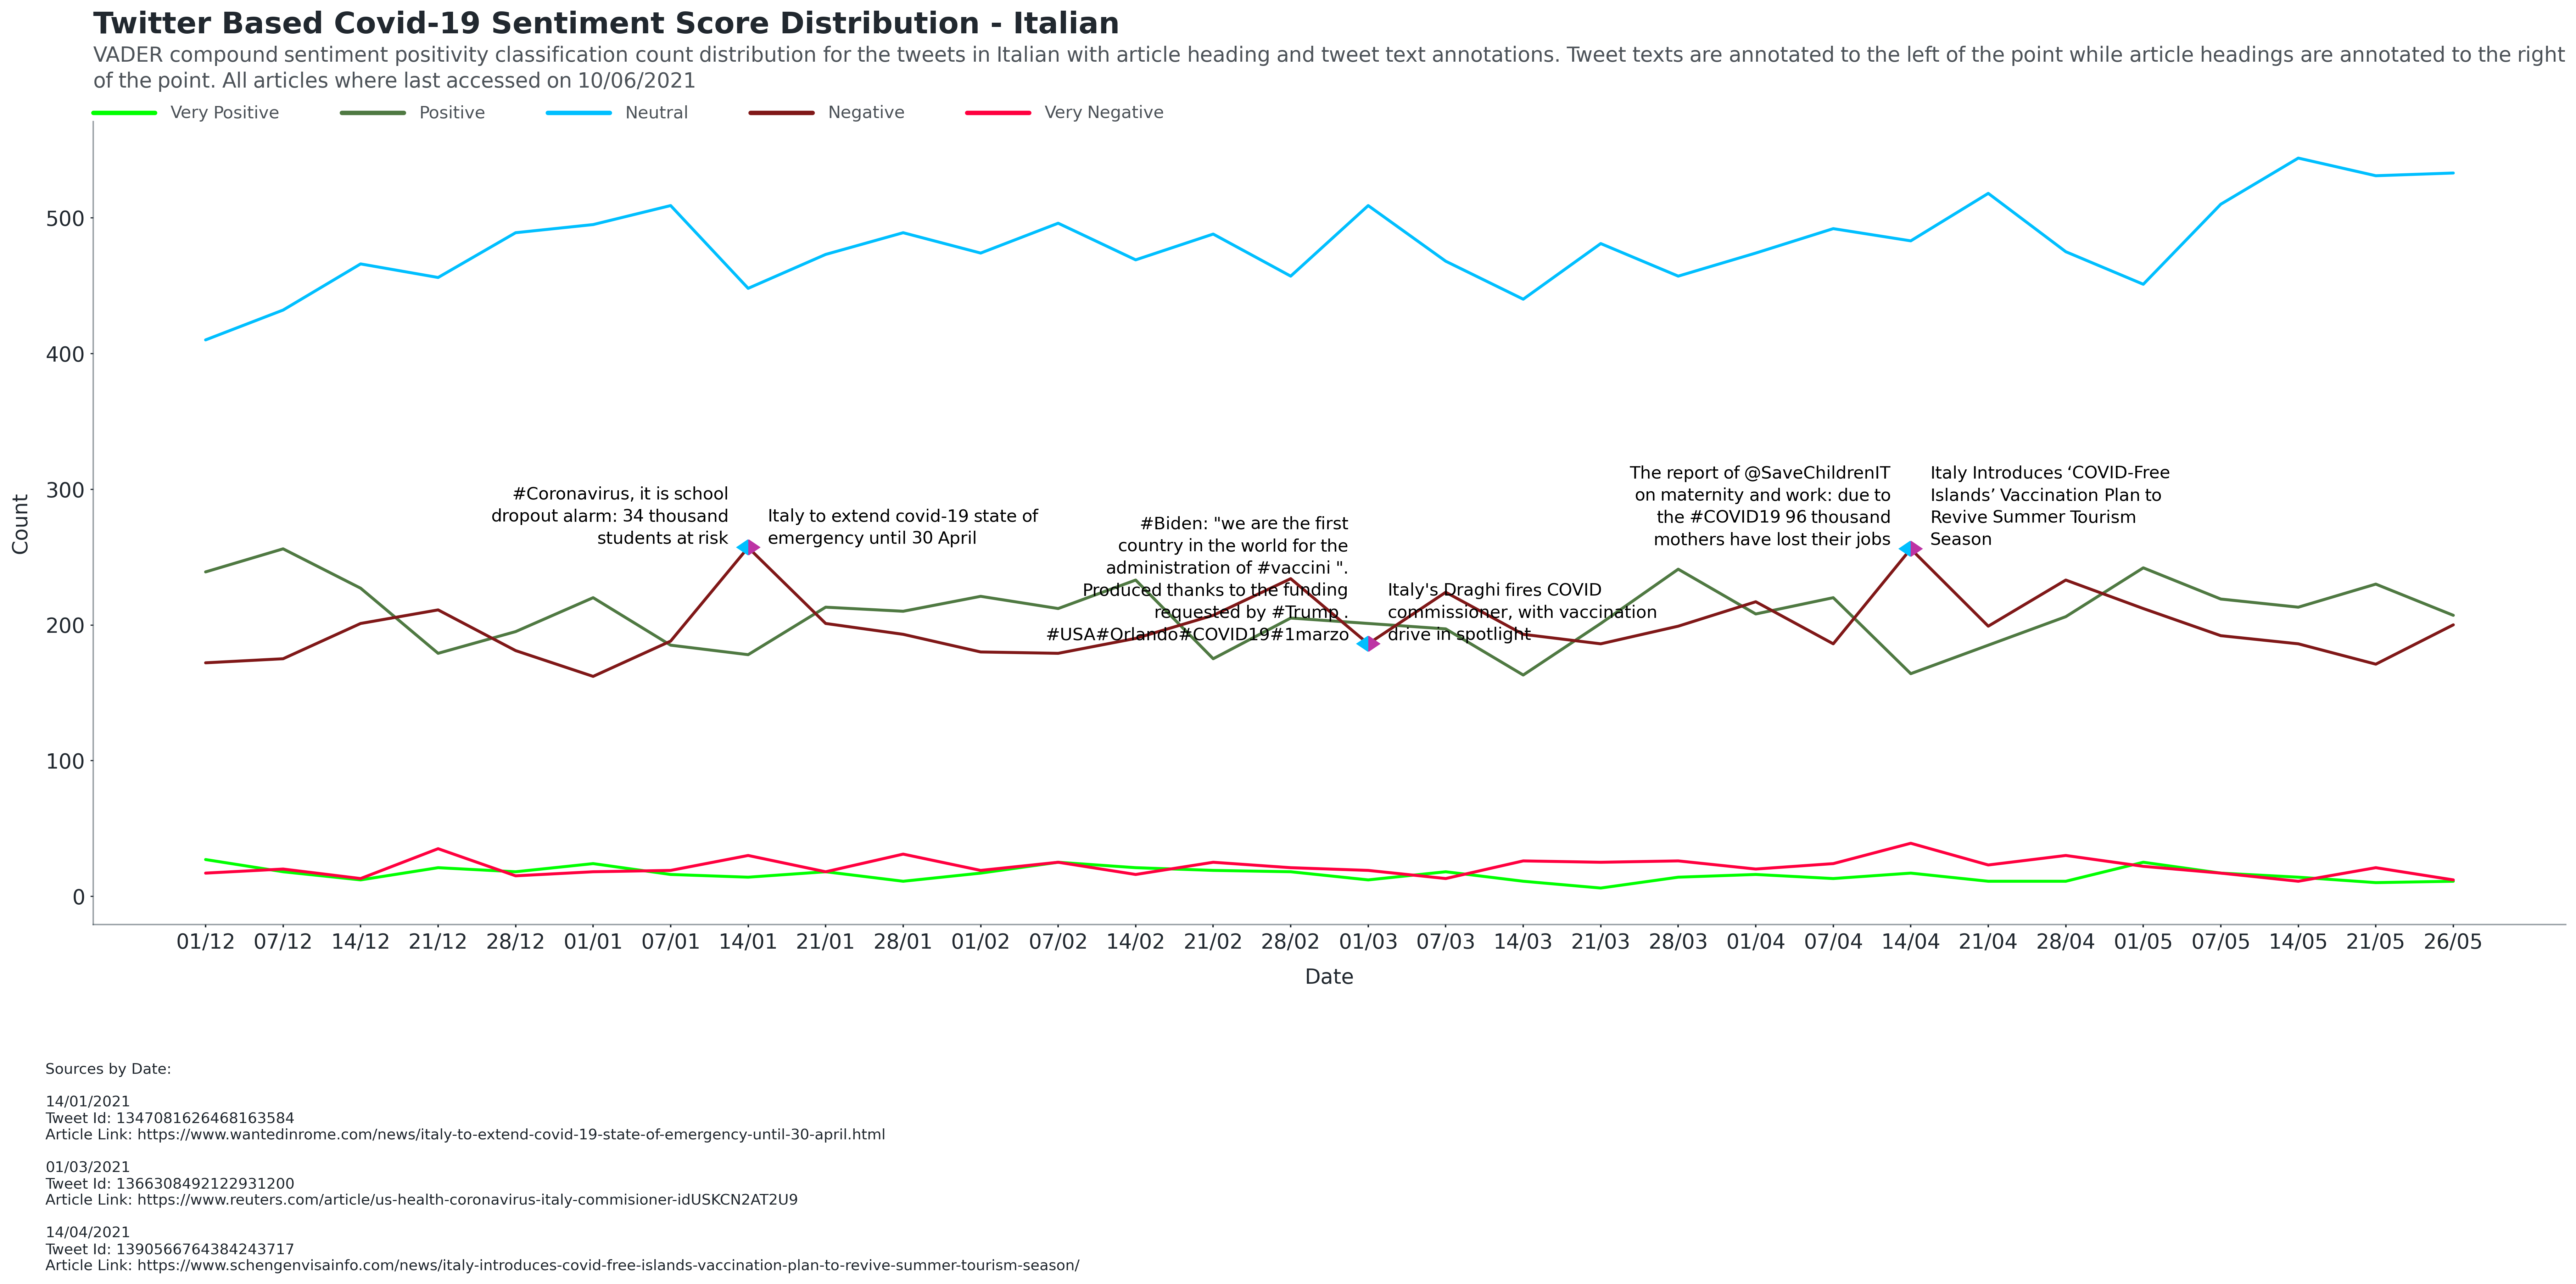
\includegraphics[scale=0.33]{Final Italian Annotated Distribution.png}
\caption[Final Italian Annotated Distribution]{ }
\label{fig:Italian}
\end{figure}

\begin{figure}[h!]
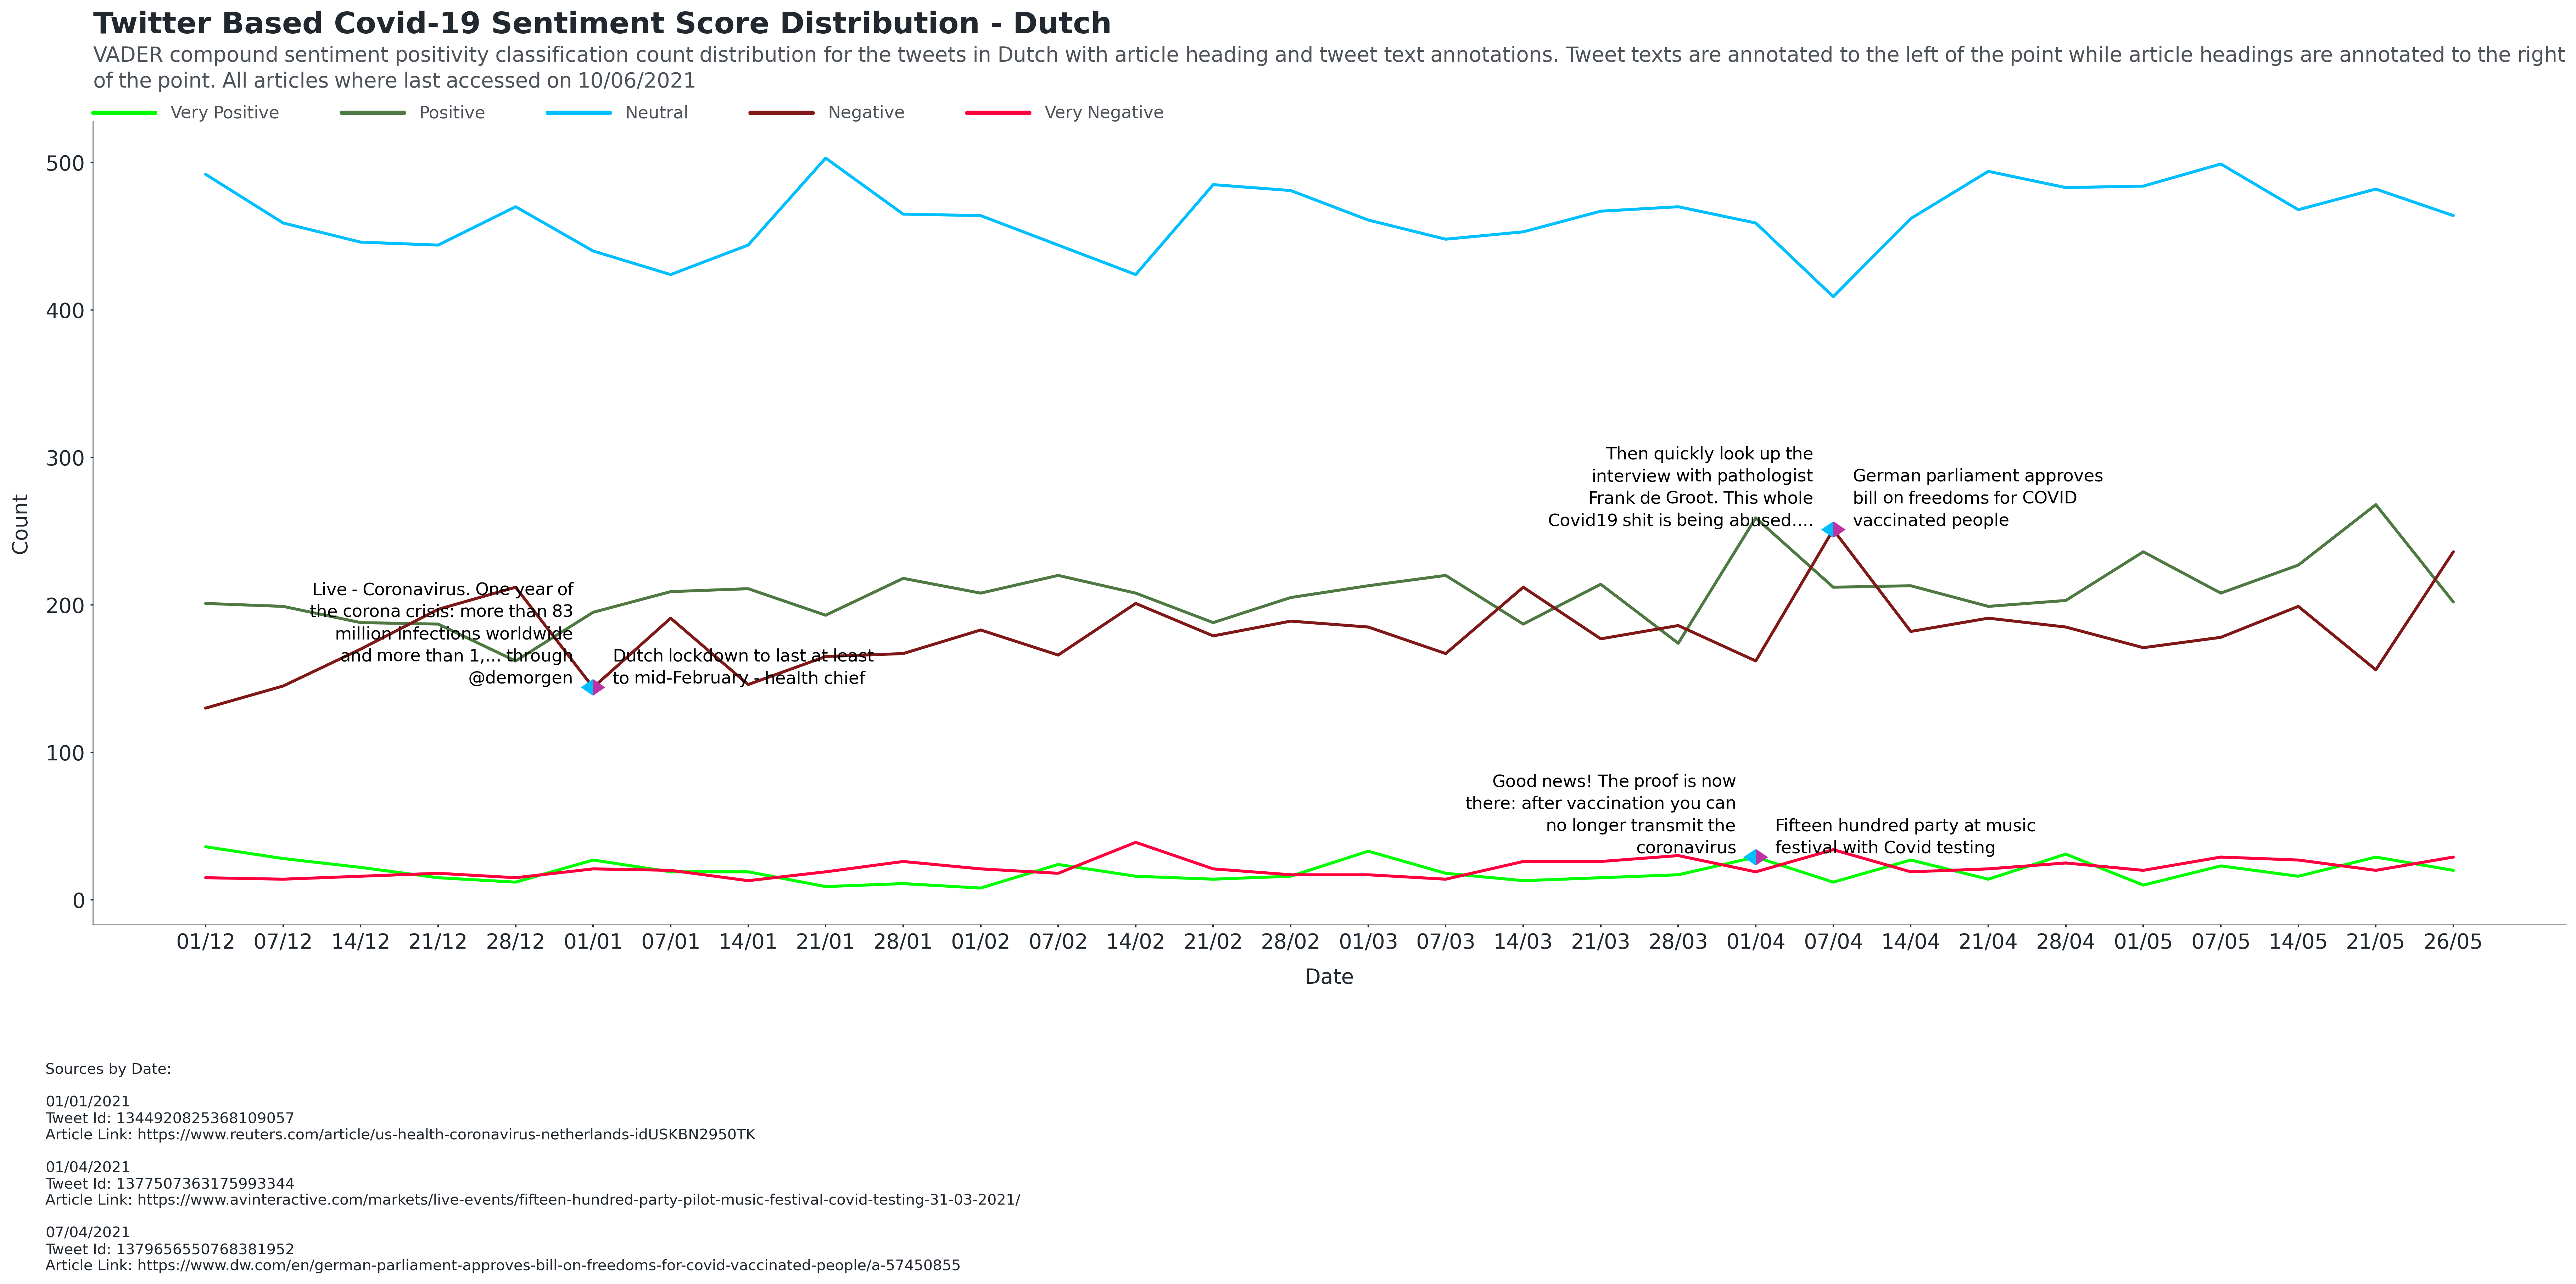
\includegraphics[scale=0.33]{Final Dutch Annotated Distribution.png}
\caption[Final Dutch Annotated Distribution]{ }
\label{fig:Dutch}
\end{figure}

%\noindent For figure~\ref{fig:Dutch}

\newpage

\section{Daily Article vs Twitter Mean Sentiment}

To see the relationship news articles and tweets have the daily mean sentiment scores of each language where plotted.

\begin{figure}[h!]
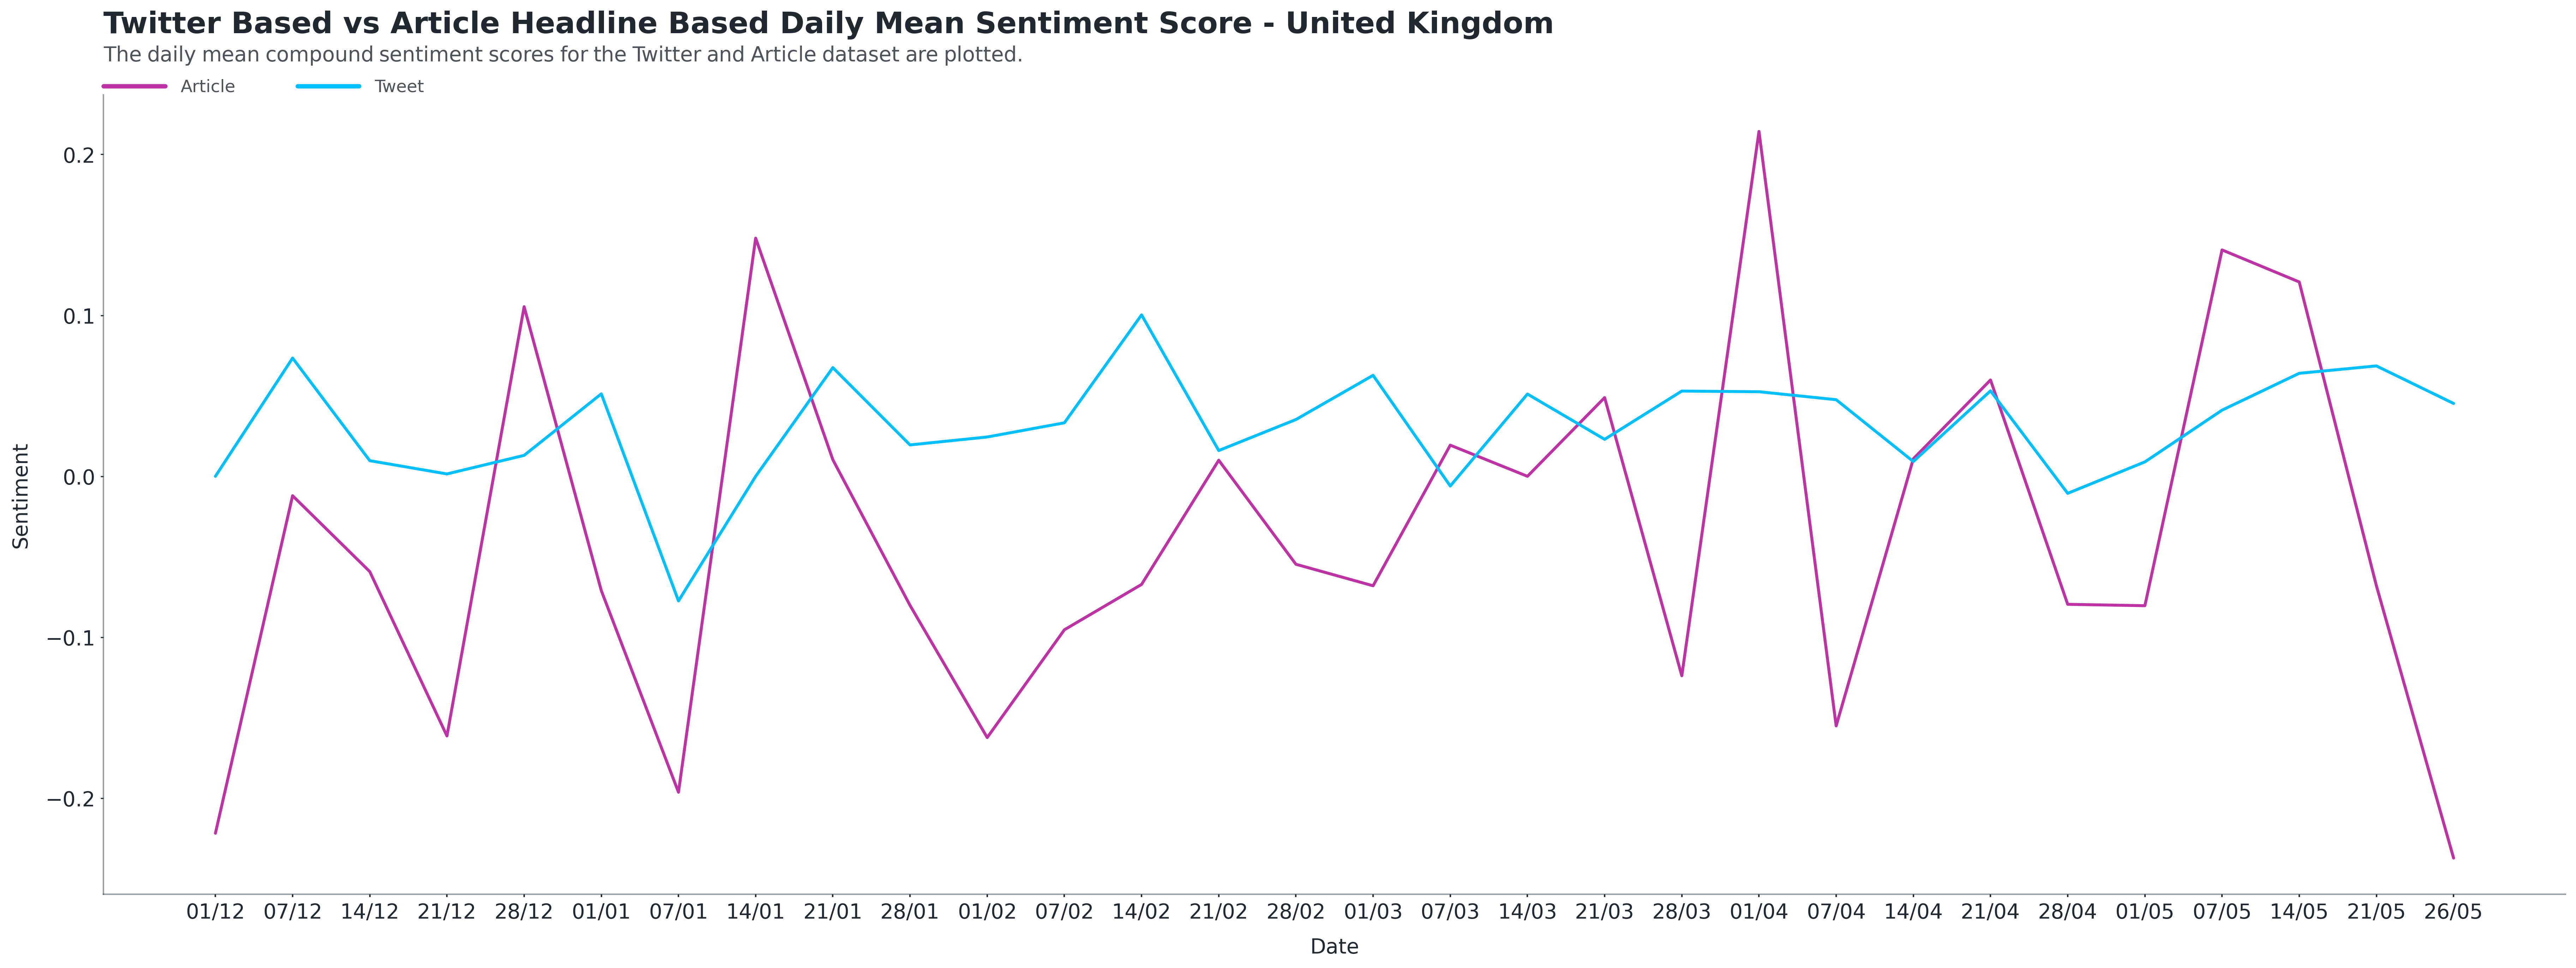
\includegraphics[scale=0.33]{Daily Mean Article VS Twitter UK.png}
\caption[Daily Mean Article VS Twitter]{ }
\label{fig:artcilevstwitteruk}
\end{figure}

\begin{figure}[h!]
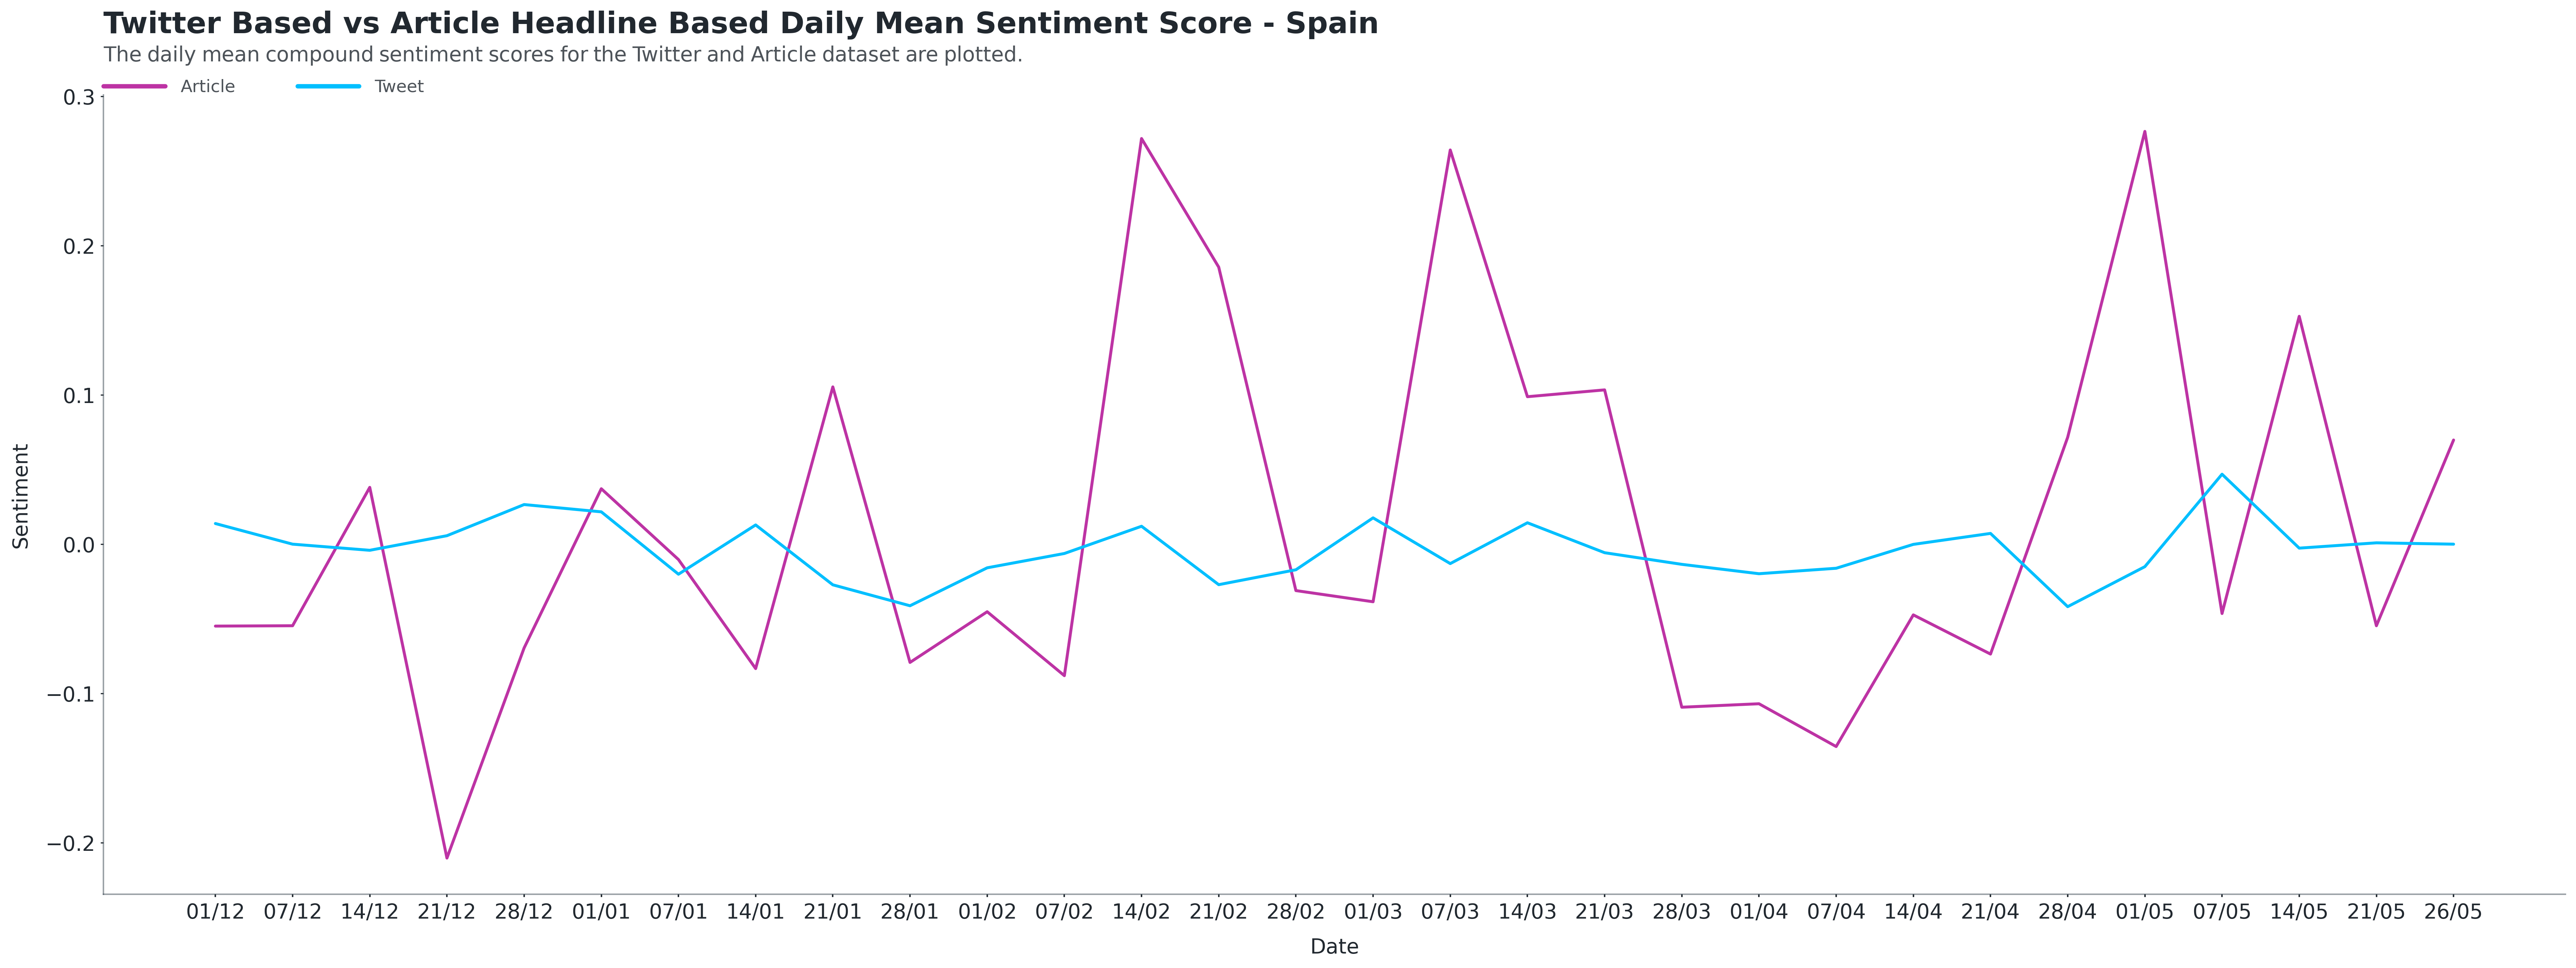
\includegraphics[scale=0.33]{Daily Mean Article VS Twitter Spain.png}
\caption[Daily Mean Article VS Twitter]{ }
\label{fig:artcilevstwitteres}
\end{figure}

\begin{figure}[h!]
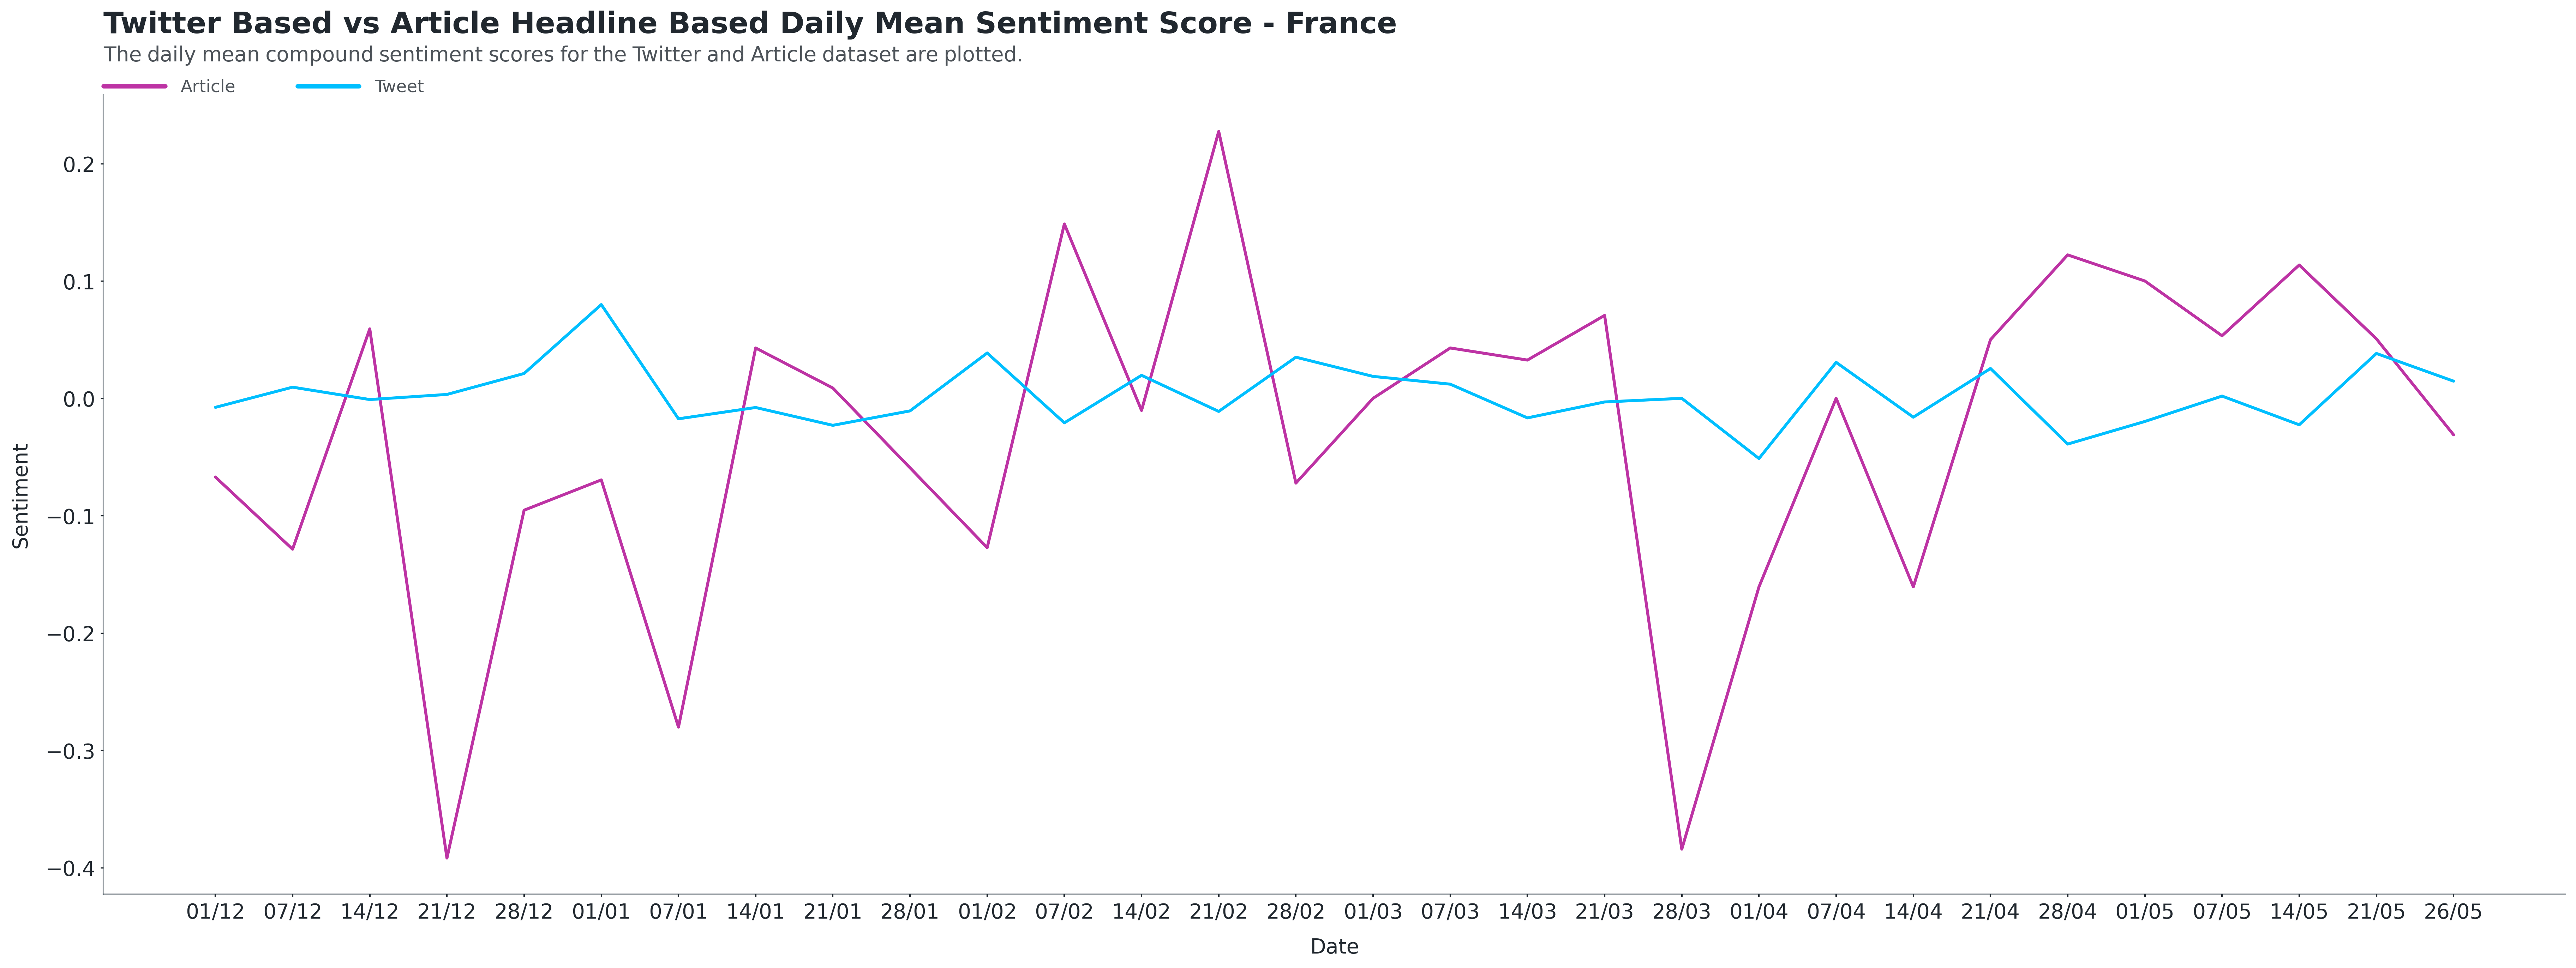
\includegraphics[scale=0.33]{Daily Mean Article VS Twitter France.png}
\caption[Daily Mean Article VS Twitter]{ }
\label{fig:artcilevstwitterfr}
\end{figure}

\begin{figure}[h!]
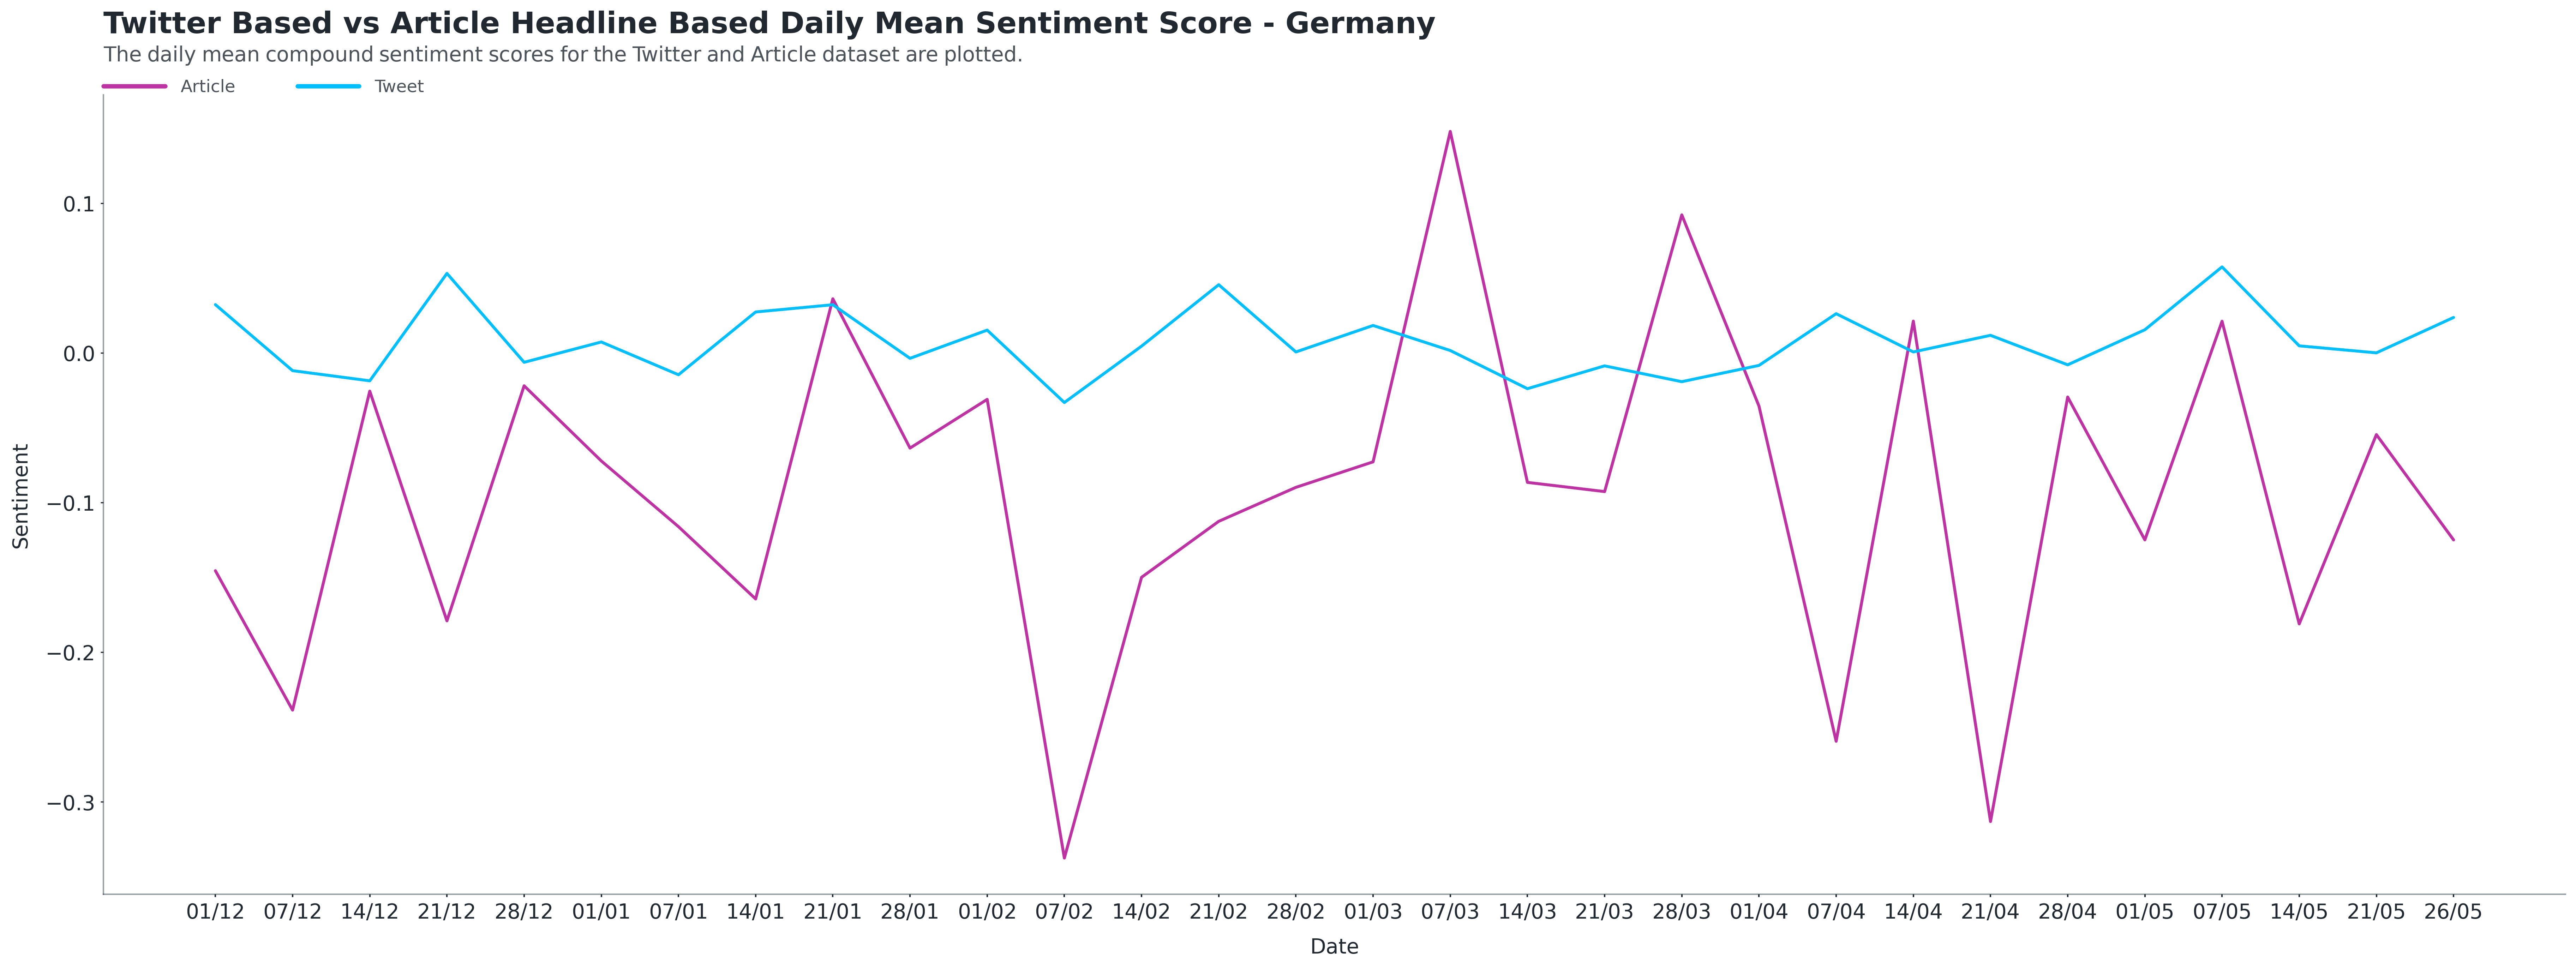
\includegraphics[scale=0.33]{Daily Mean Article VS Twitter Germany.png}
\caption[Daily Mean Article VS Twitter]{ }
\label{fig:artcilevstwitterde}
\end{figure}

\begin{figure}[h!]
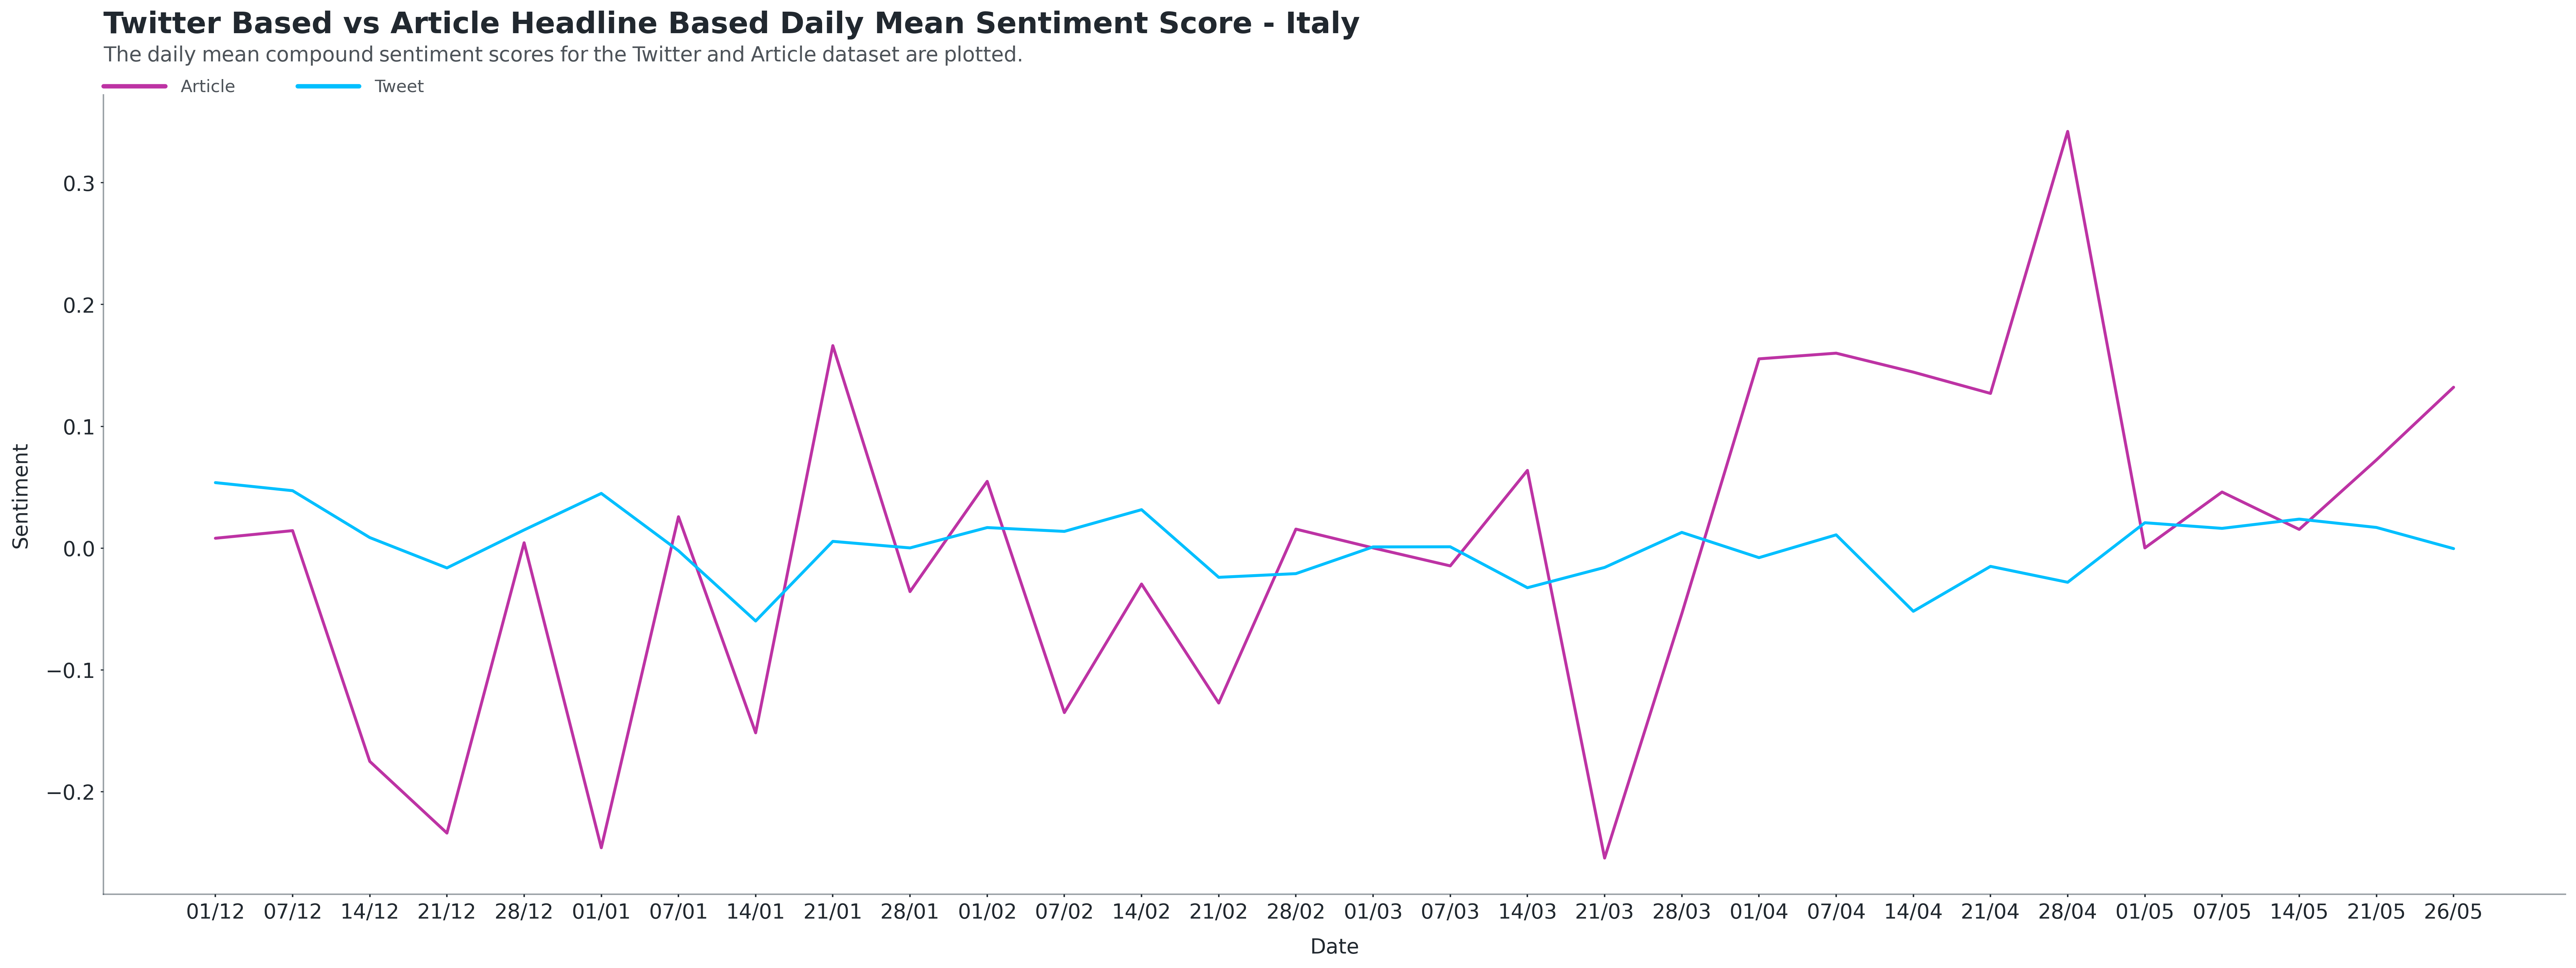
\includegraphics[scale=0.33]{Daily Mean Article VS Twitter Italy.png}
\caption[Daily Mean Article VS Twitter]{ }
\label{fig:artcilevstwitterit}
\end{figure}

\begin{figure}[h!]
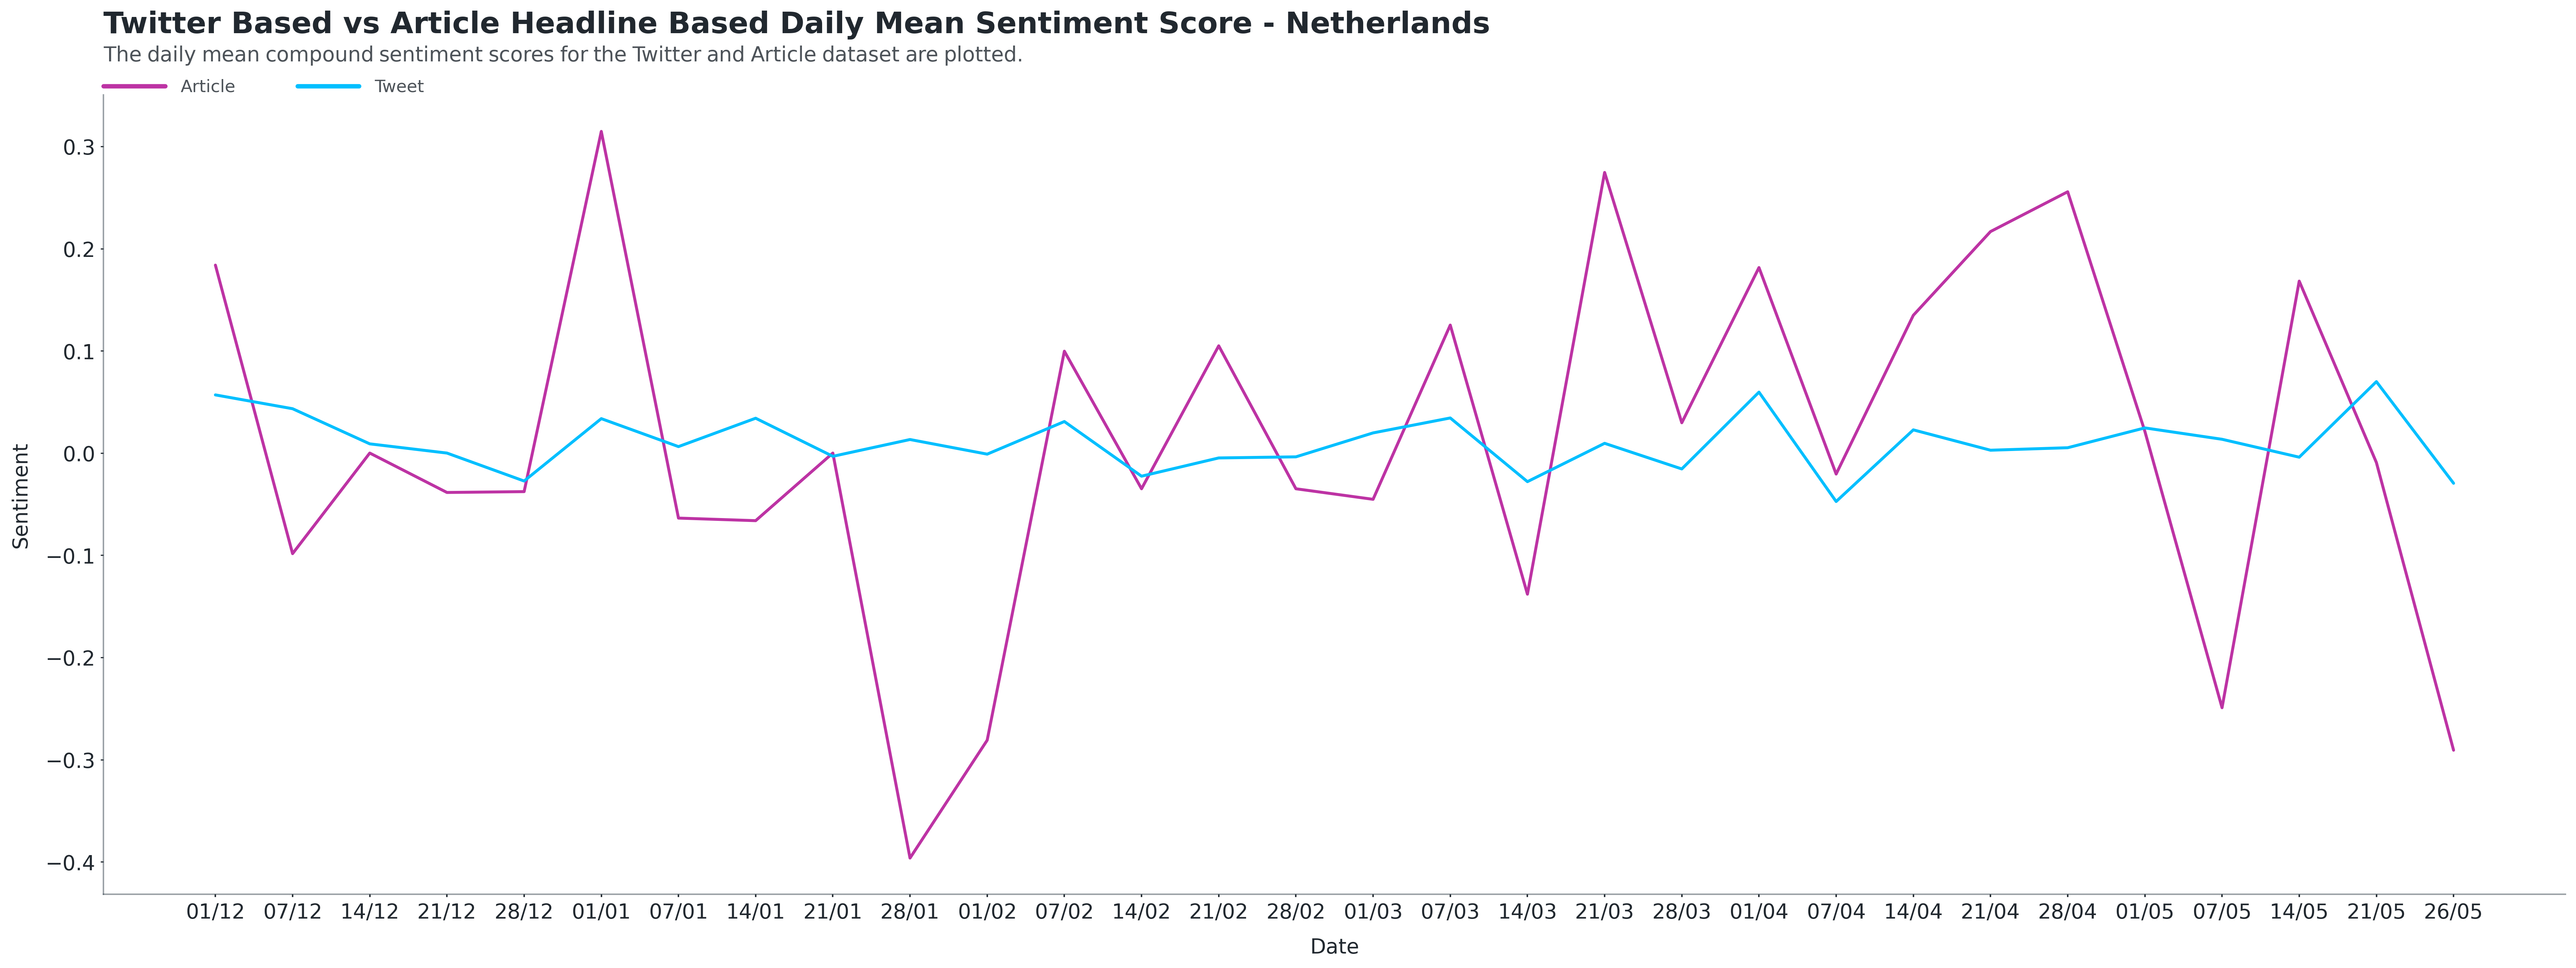
\includegraphics[scale=0.33]{Daily Mean Article VS Twitter Netherlands.png}
\caption[Daily Mean Article VS Twitter]{ }
\label{fig:artcilevstwitternl}
\end{figure}

\newpage

\section{Word Frequency in the Form of Word Clouds}

Finally the a word cloud was generated for each month in each language.
These word clouds where used to follow the difference of word usage over the 6 month period.


\begin{figure}[!htb]
\minipage{0.33\textwidth}
  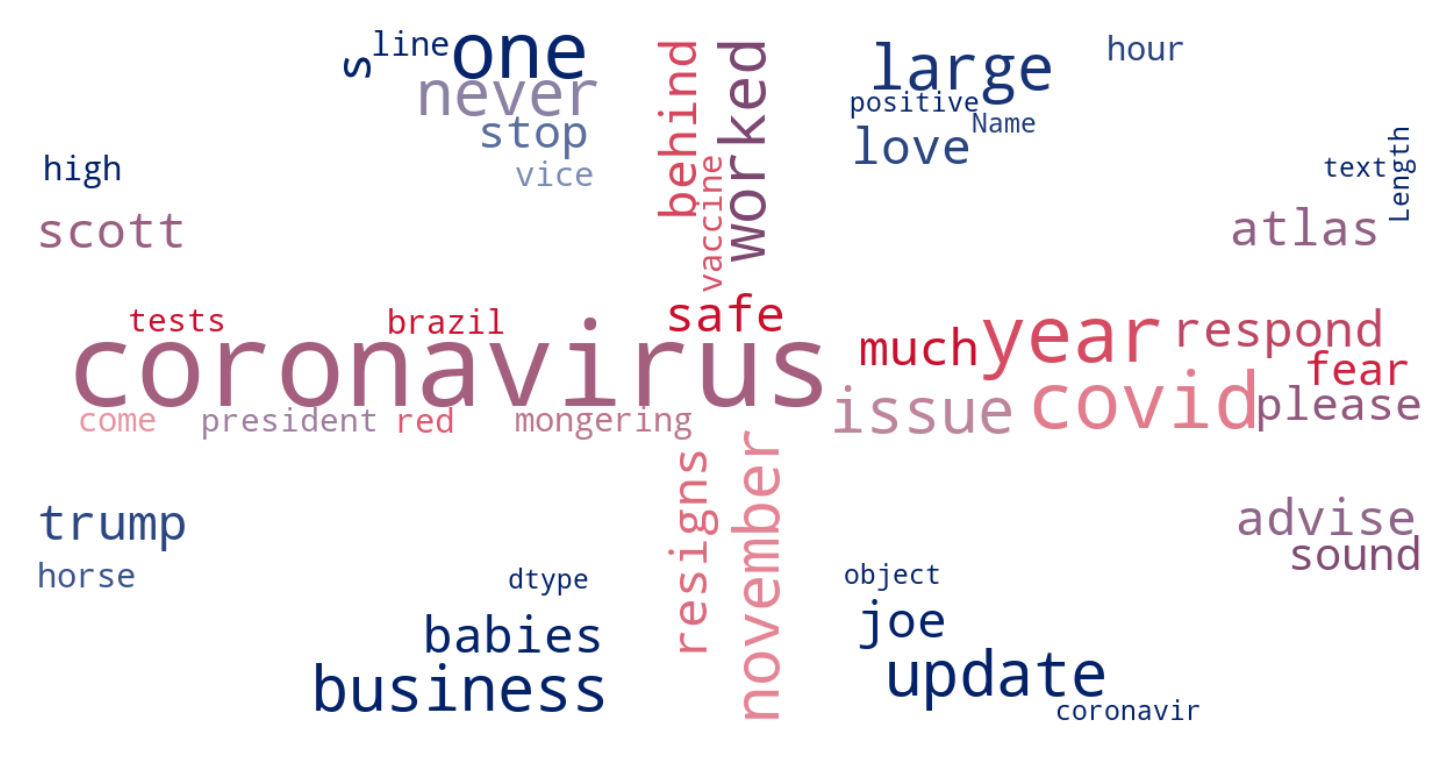
\includegraphics[width=\linewidth]{December en word cloud.png}
  \caption{English word cloud in December}\label{fig:decemberUK}
\endminipage\hfill
\minipage{0.33\textwidth}
  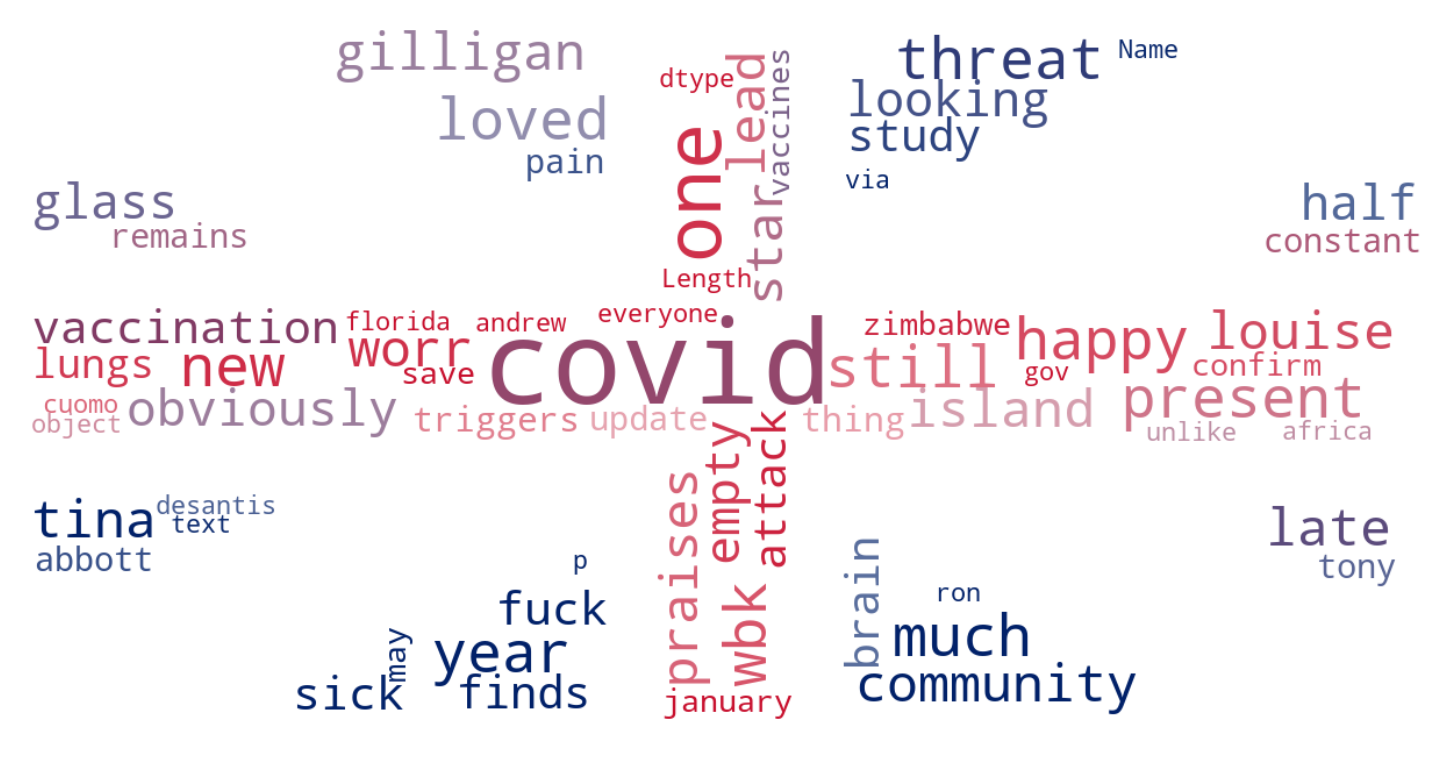
\includegraphics[width=\linewidth]{January en word cloud.png}
  \caption{English word cloud in January}\label{fig:januaryUK}
\endminipage\hfill
\minipage{0.33\textwidth}
  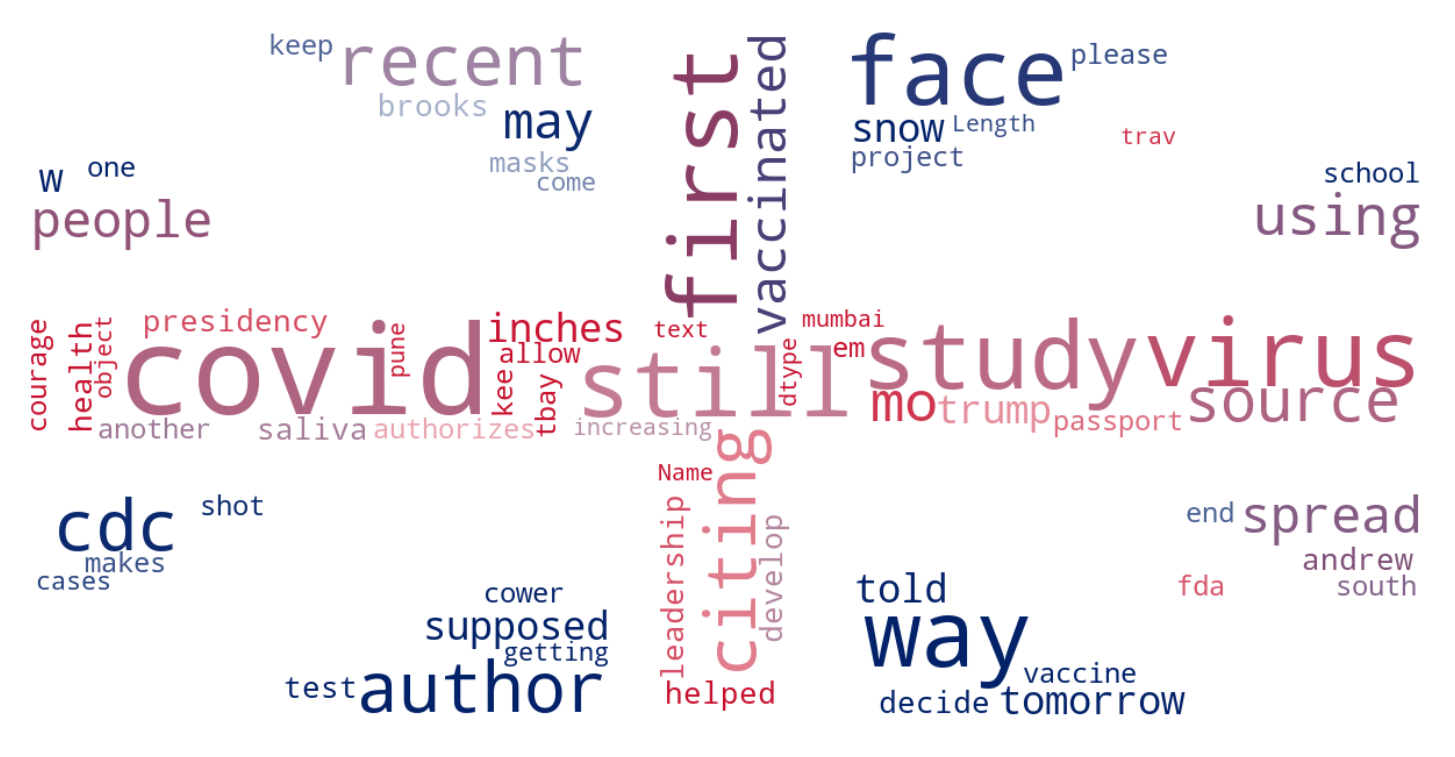
\includegraphics[width=\linewidth]{February en word cloud.png}
  \caption{English word cloud in February}\label{fig:februaryUK}
\endminipage
\end{figure}
\begin{figure}[!htb]
\minipage{0.33\textwidth}
  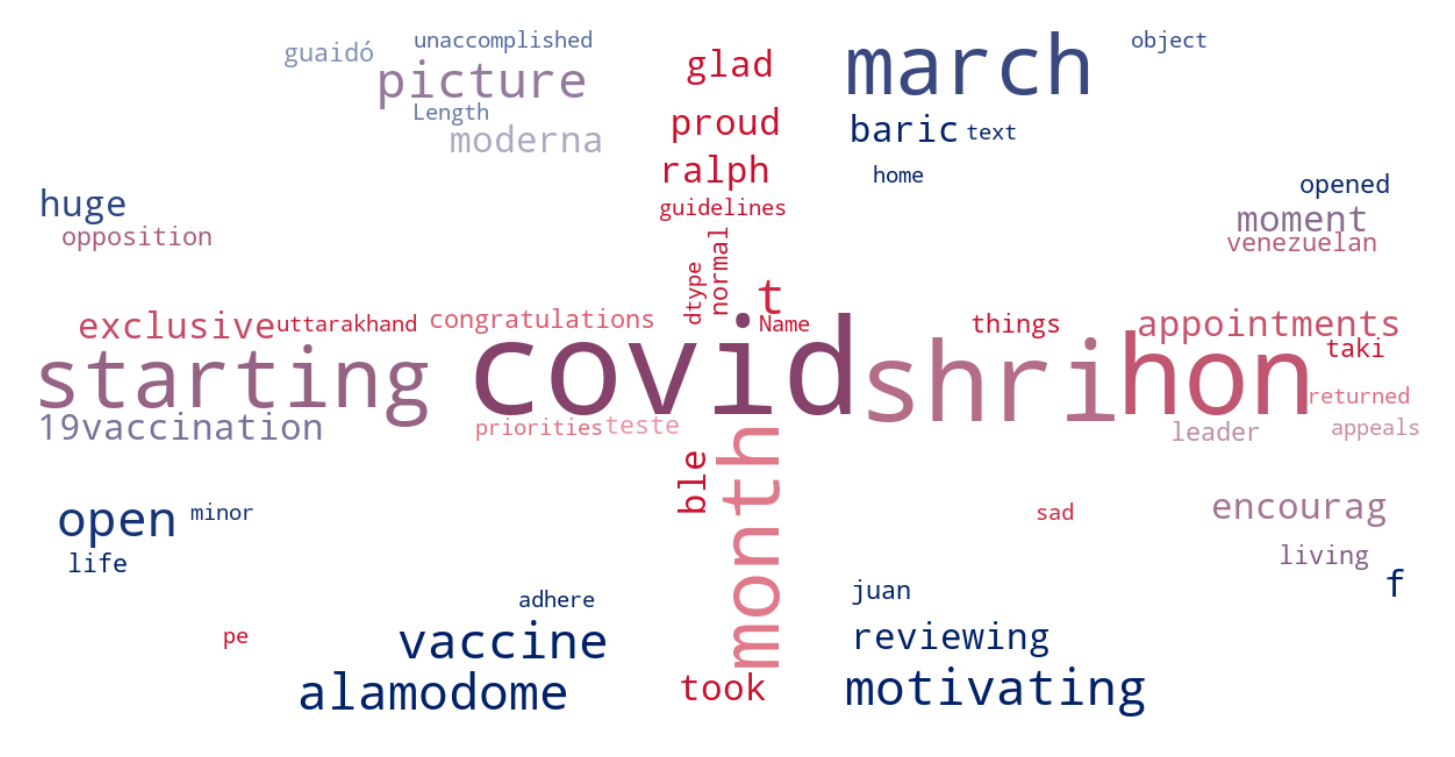
\includegraphics[width=\linewidth]{March en word cloud.png}
  \caption{English word cloud in March}\label{fig:marchUK}
\endminipage\hfill
\minipage{0.33\textwidth}
  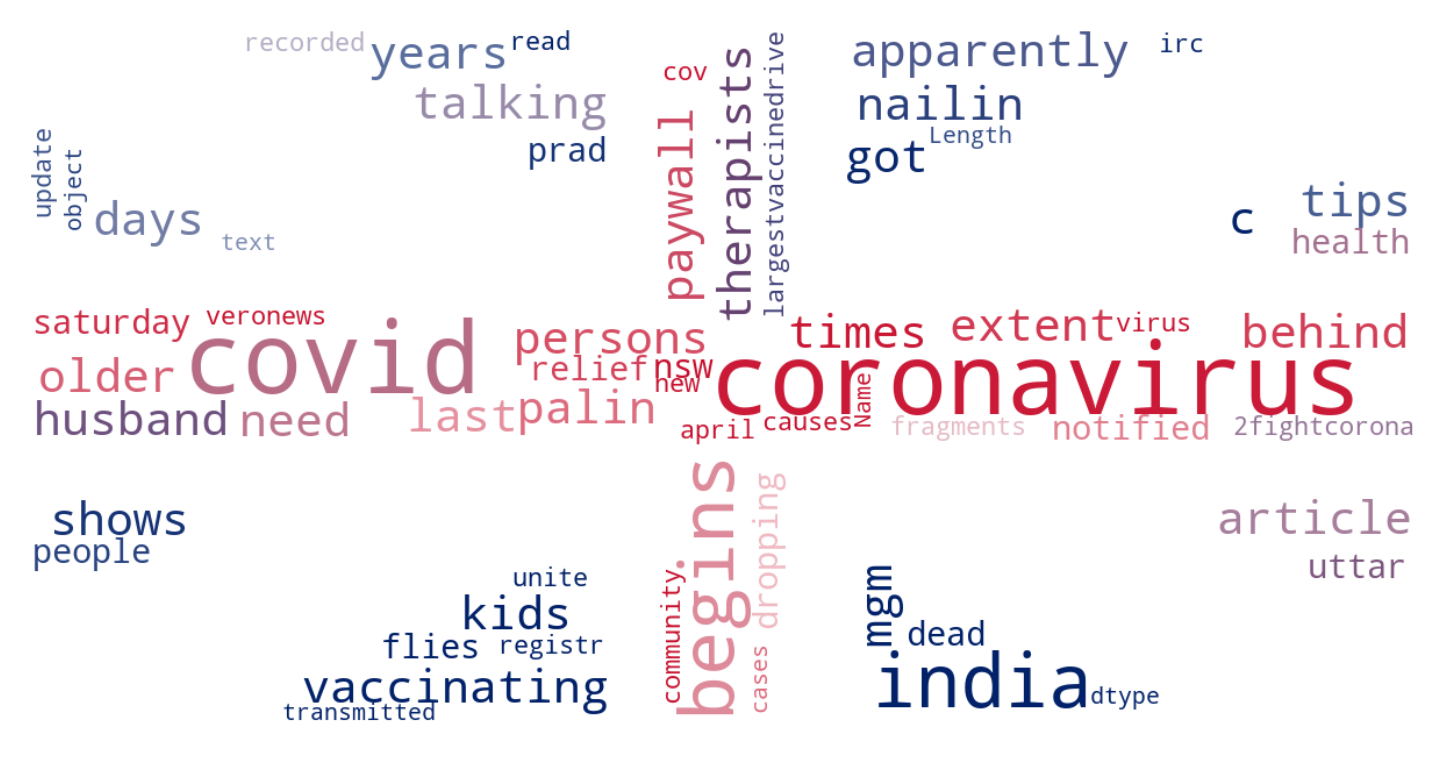
\includegraphics[width=\linewidth]{April en word cloud.png}
  \caption{English word cloud in April}\label{fig:aprilUK}
\endminipage\hfill
\minipage{0.33\textwidth}
  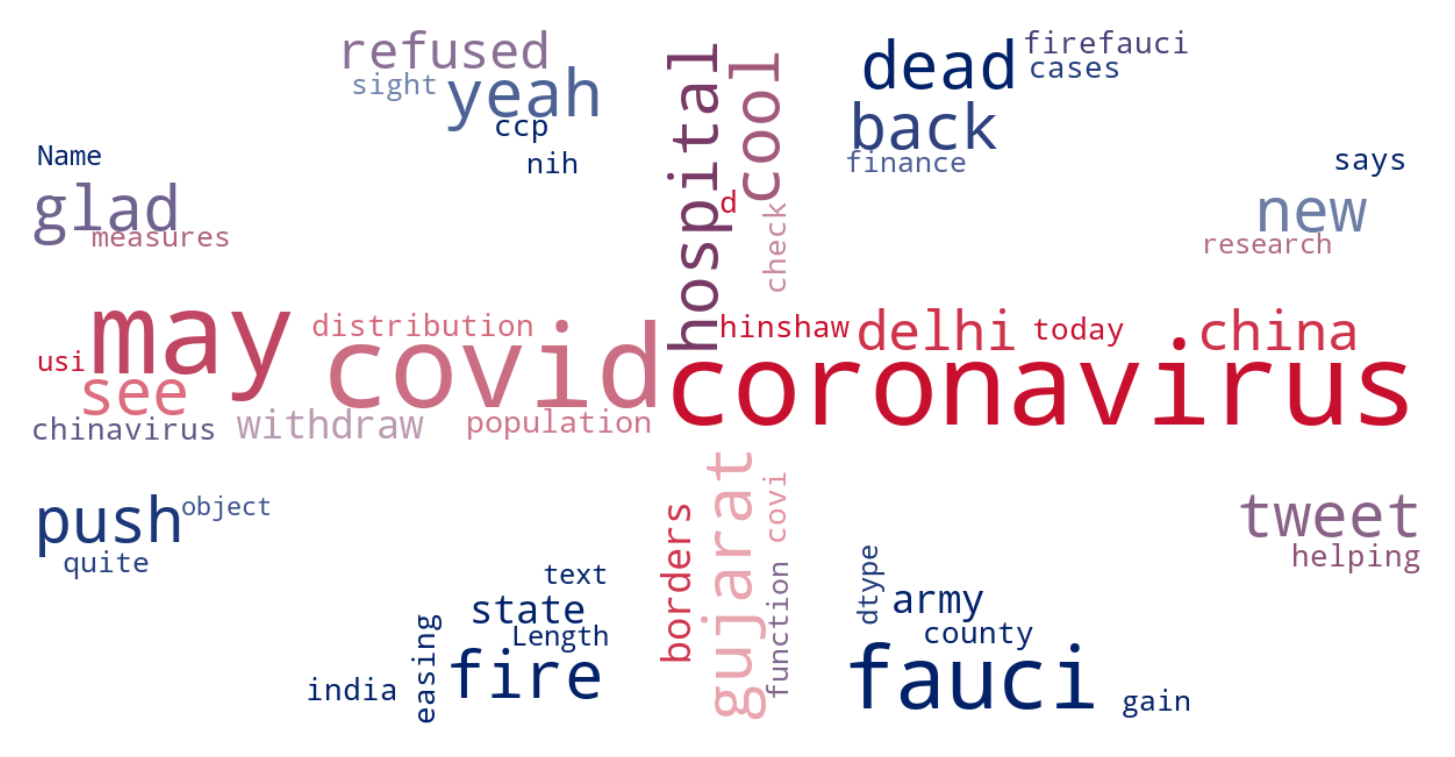
\includegraphics[width=\linewidth]{May en word cloud.png}
  \caption{English word cloud in May}\label{fig:mayUK}
\endminipage
\end{figure}


\begin{figure}[!htb]
\minipage{0.33\textwidth}
  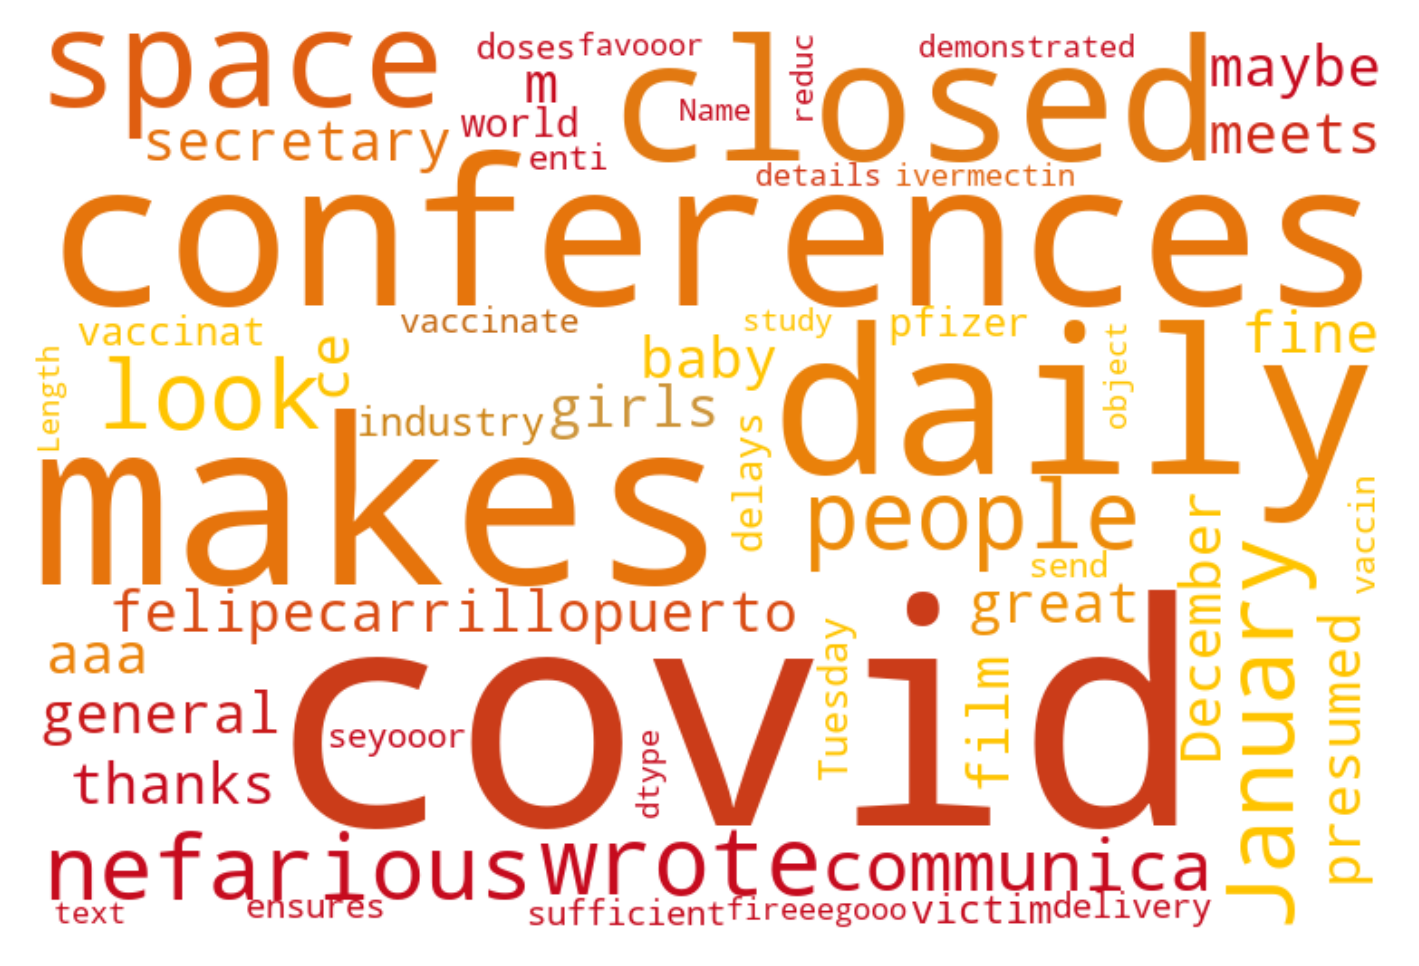
\includegraphics[width=\linewidth]{December es word cloud.png}
  \caption{Spanish word cloud in December}\label{fig:decemberes}
\endminipage\hfill
\minipage{0.33\textwidth}
  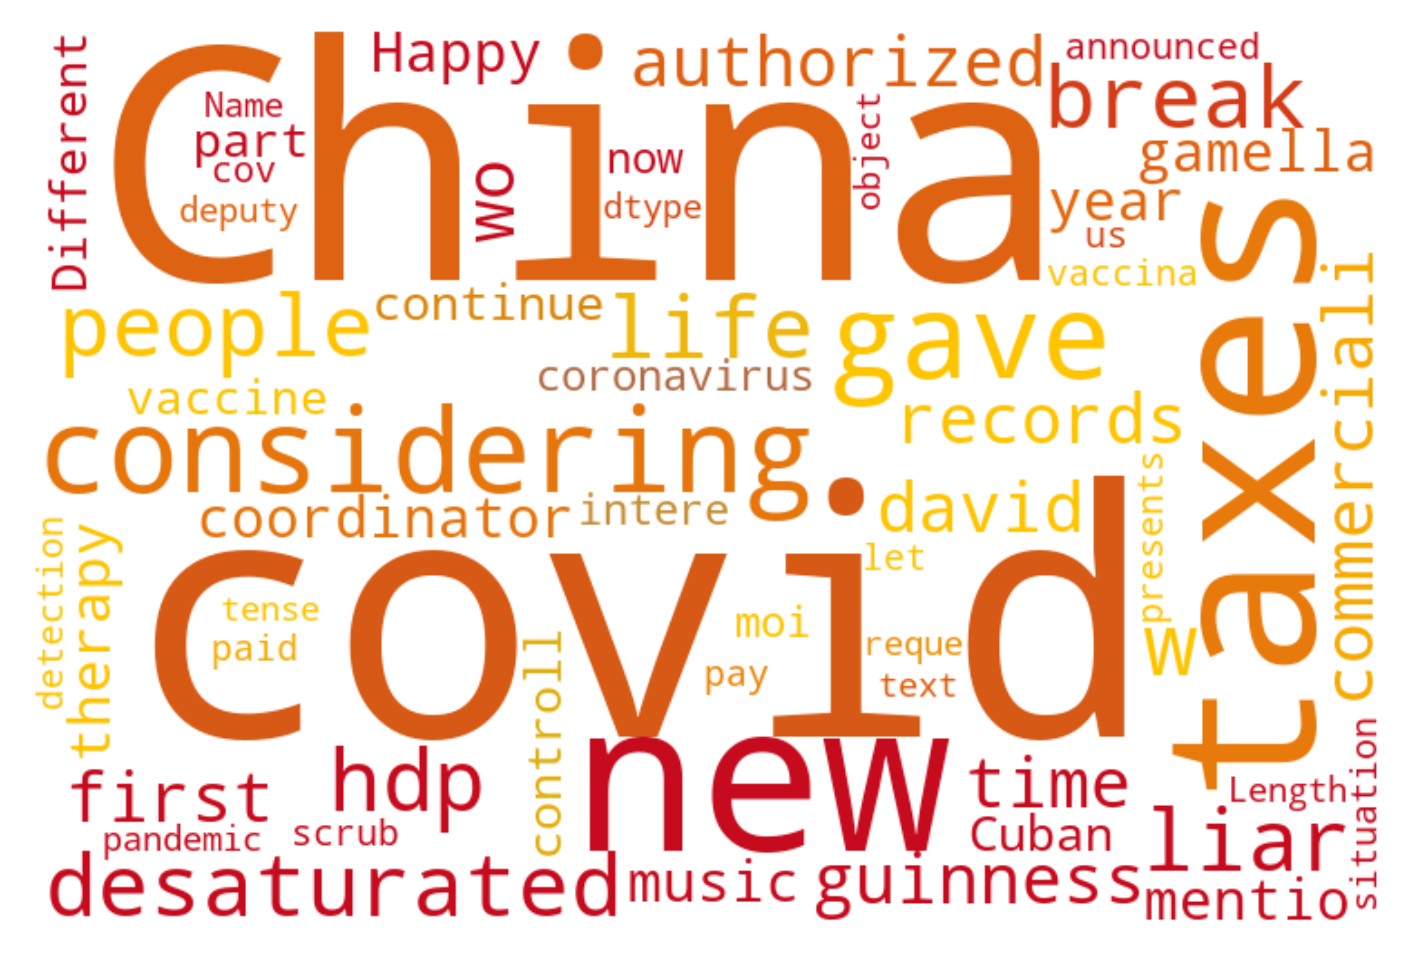
\includegraphics[width=\linewidth]{January es word cloud.png}
  \caption{Spanish word cloud in January}\label{fig:januaryes}
\endminipage\hfill
\minipage{0.33\textwidth}
  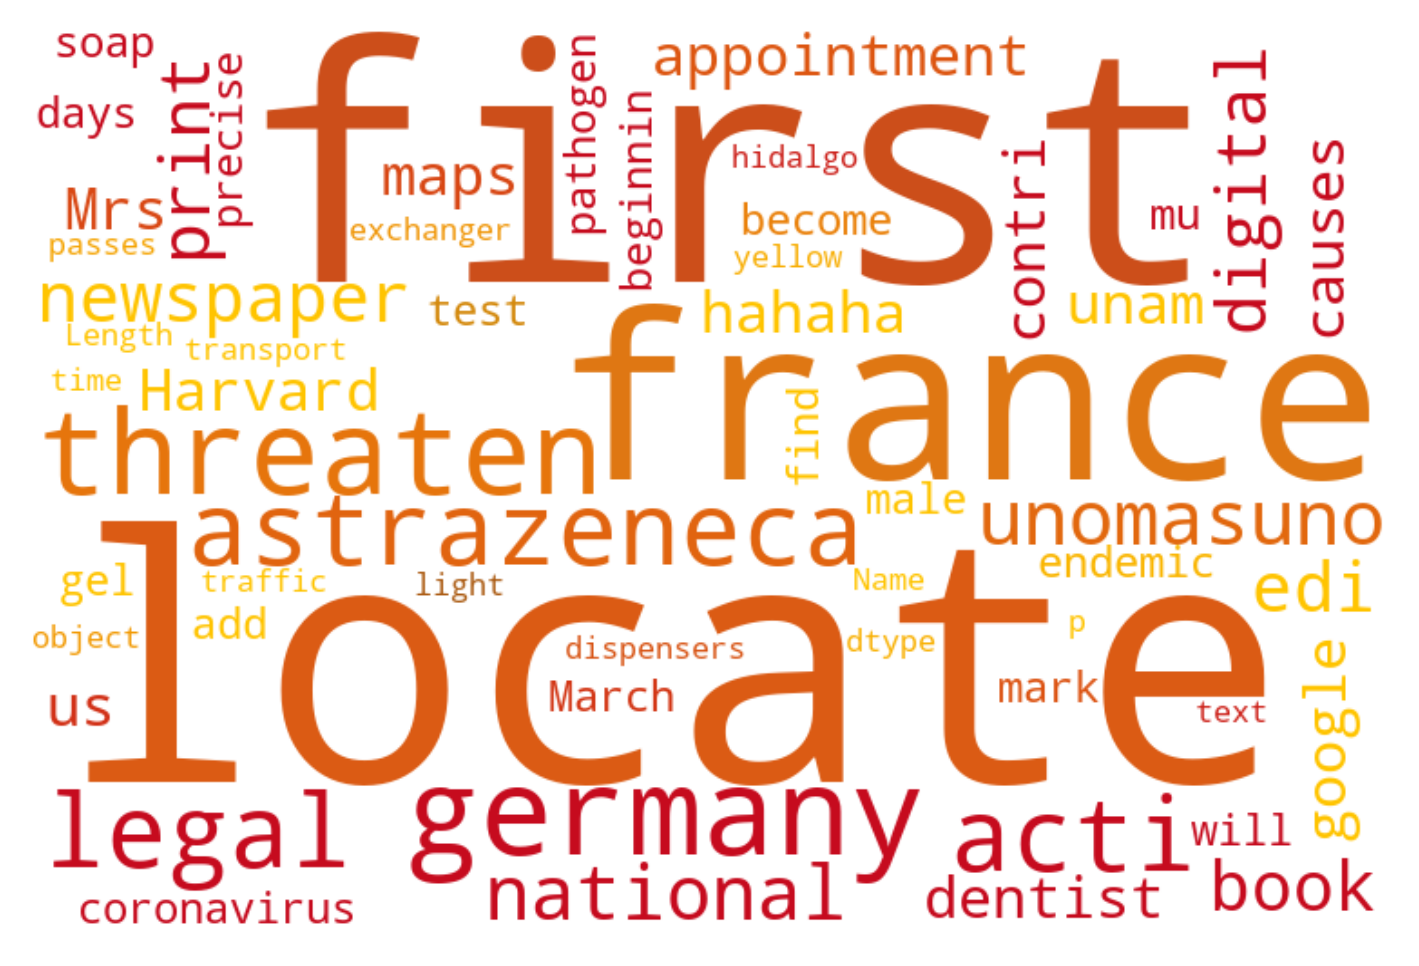
\includegraphics[width=\linewidth]{February es word cloud.png}
  \caption{Spanish word cloud in February}\label{fig:februaryes}
\endminipage
\end{figure}
\begin{figure}[!htb]
\minipage{0.33\textwidth}
  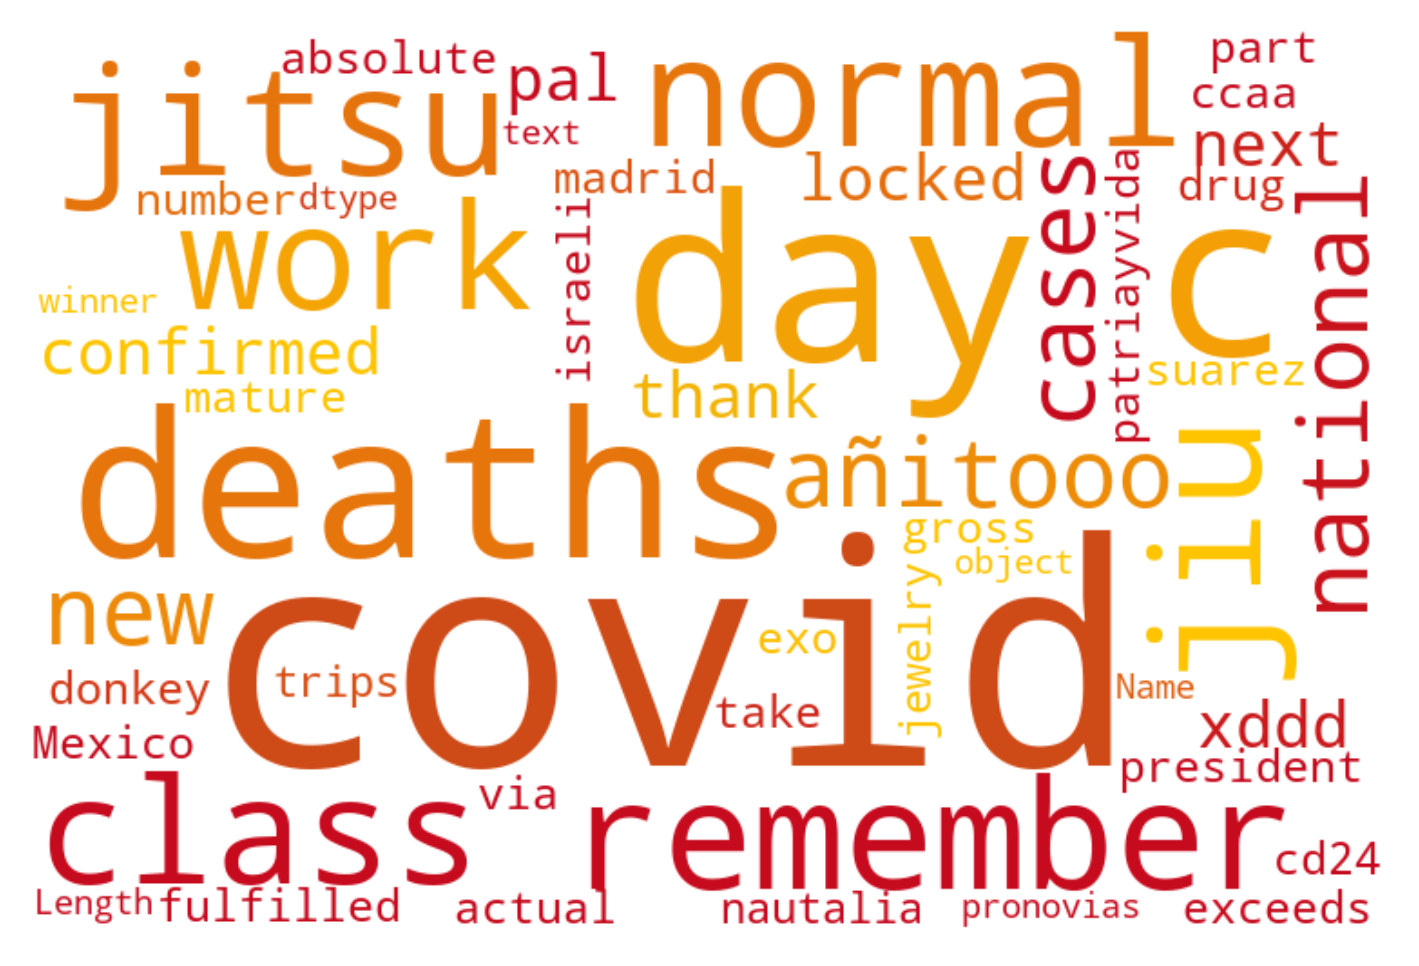
\includegraphics[width=\linewidth]{March es word cloud.png}
  \caption{Spanish word cloud in March}\label{fig:marches}
\endminipage\hfill
\minipage{0.33\textwidth}
  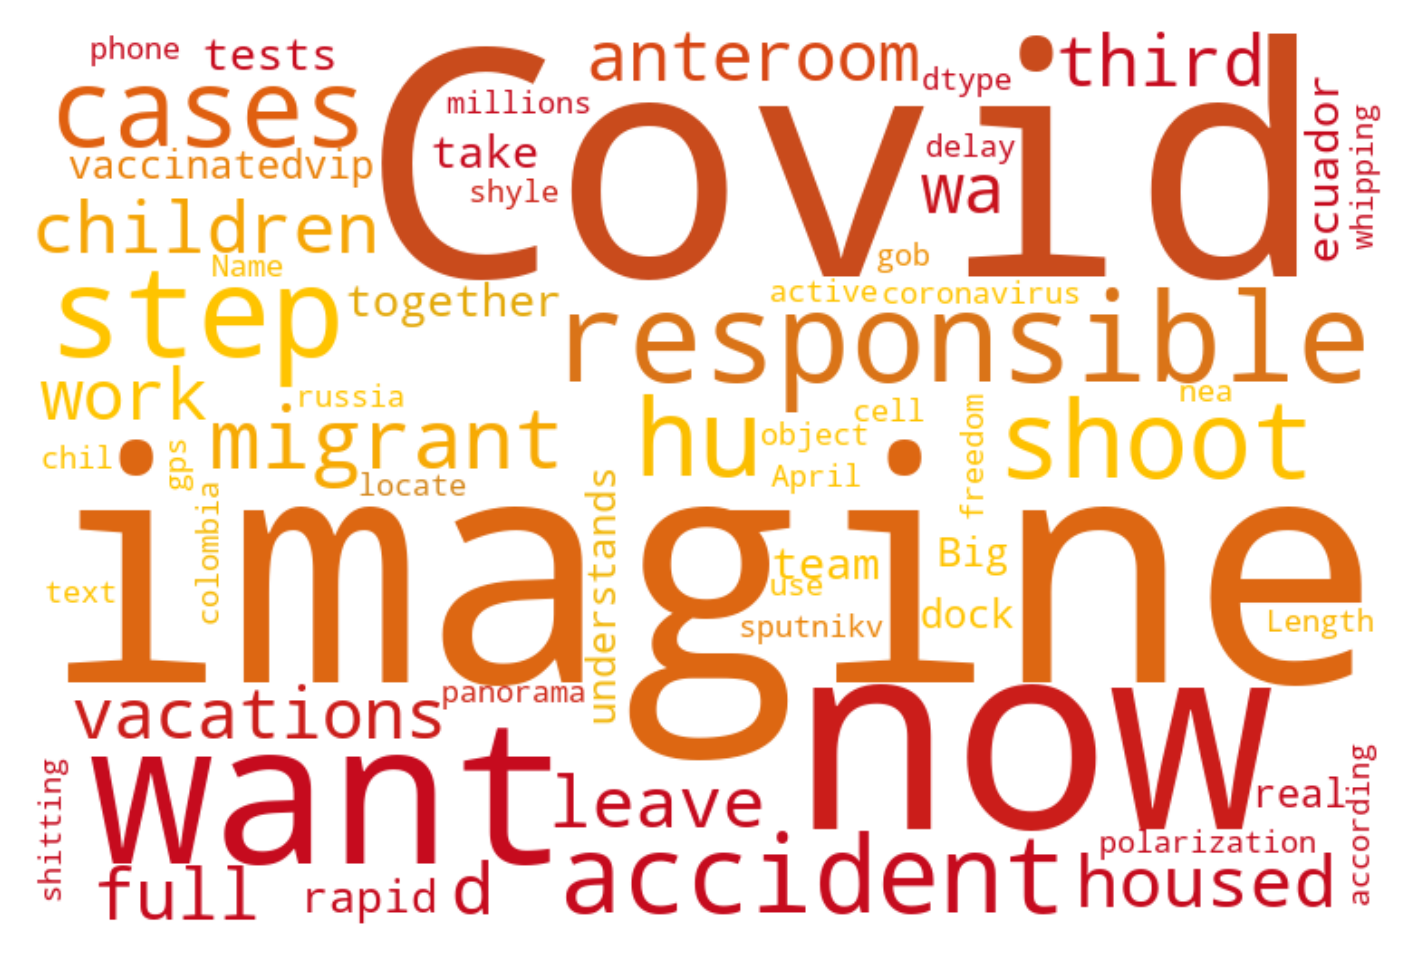
\includegraphics[width=\linewidth]{April es word cloud.png}
  \caption{Spanish word cloud in April}\label{fig:apriles}
\endminipage\hfill
\minipage{0.33\textwidth}
  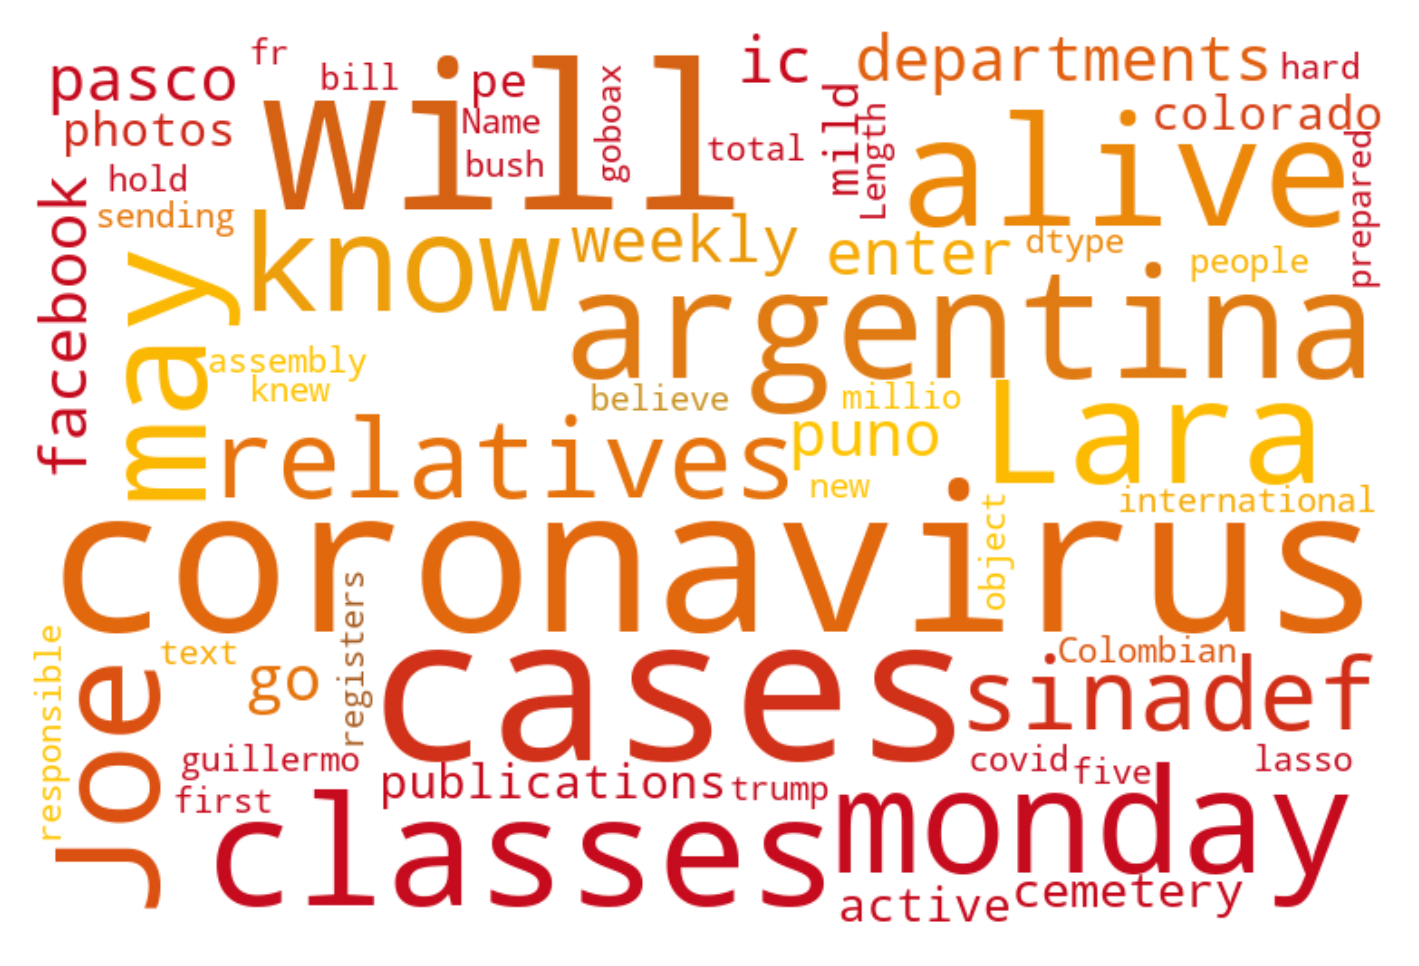
\includegraphics[width=\linewidth]{May es word cloud.png}
  \caption{Spanish word cloud in May}\label{fig:mayes}
\endminipage
\end{figure}

\begin{figure}[!htb]
\minipage{0.33\textwidth}
  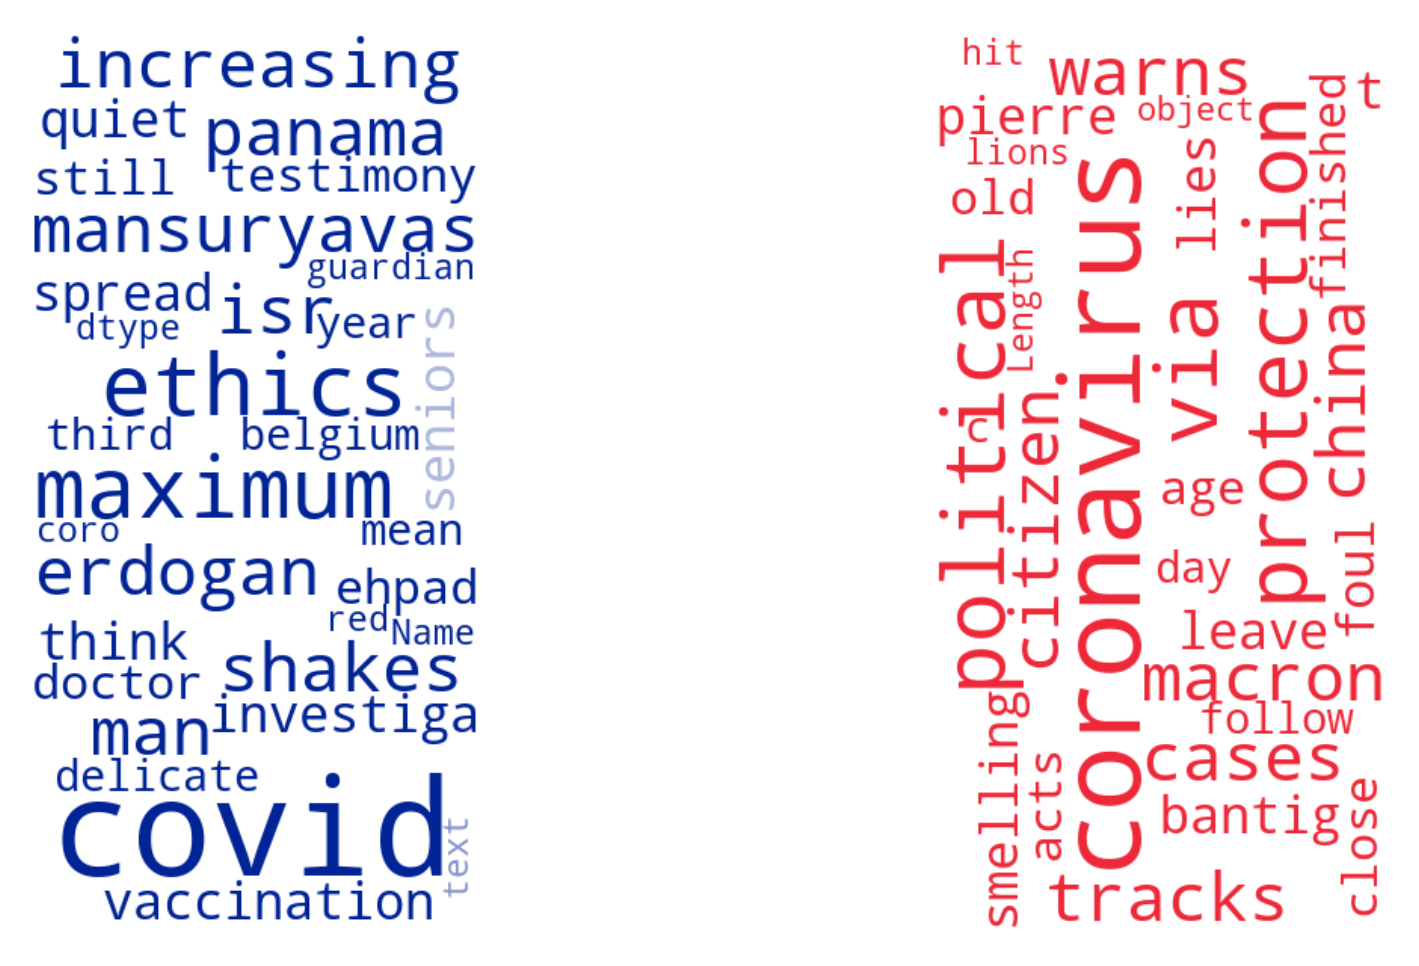
\includegraphics[width=\linewidth]{December fr word cloud.png}
  \caption{French word cloud in December}\label{fig:decemberfr}
\endminipage\hfill
\minipage{0.33\textwidth}
  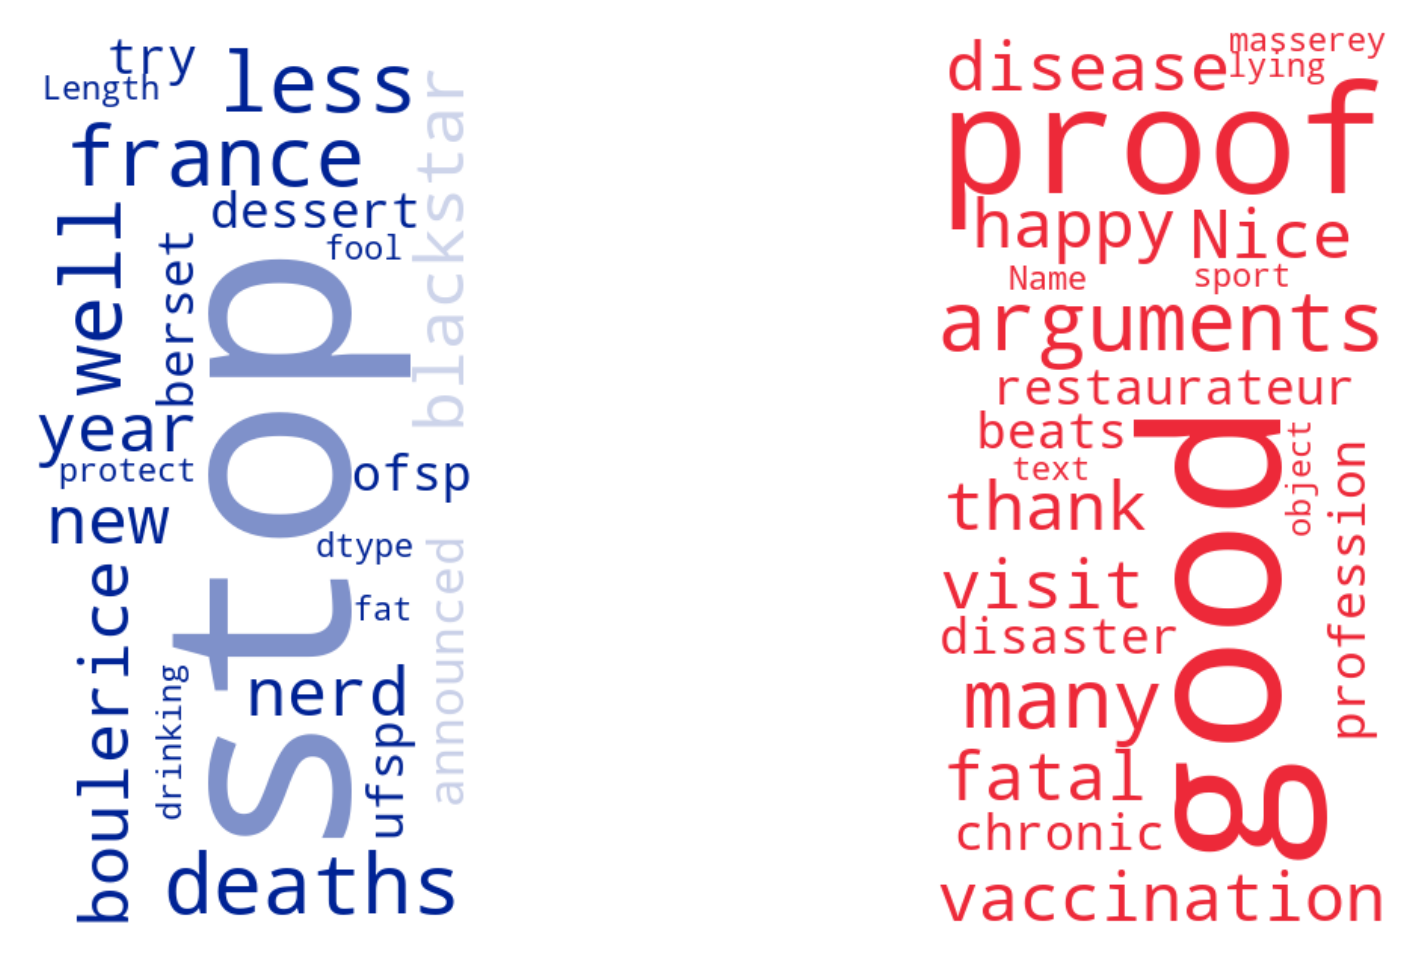
\includegraphics[width=\linewidth]{January fr word cloud.png}
  \caption{French word cloud in January}\label{fig:januaryfr}
\endminipage\hfill
\minipage{0.33\textwidth}
  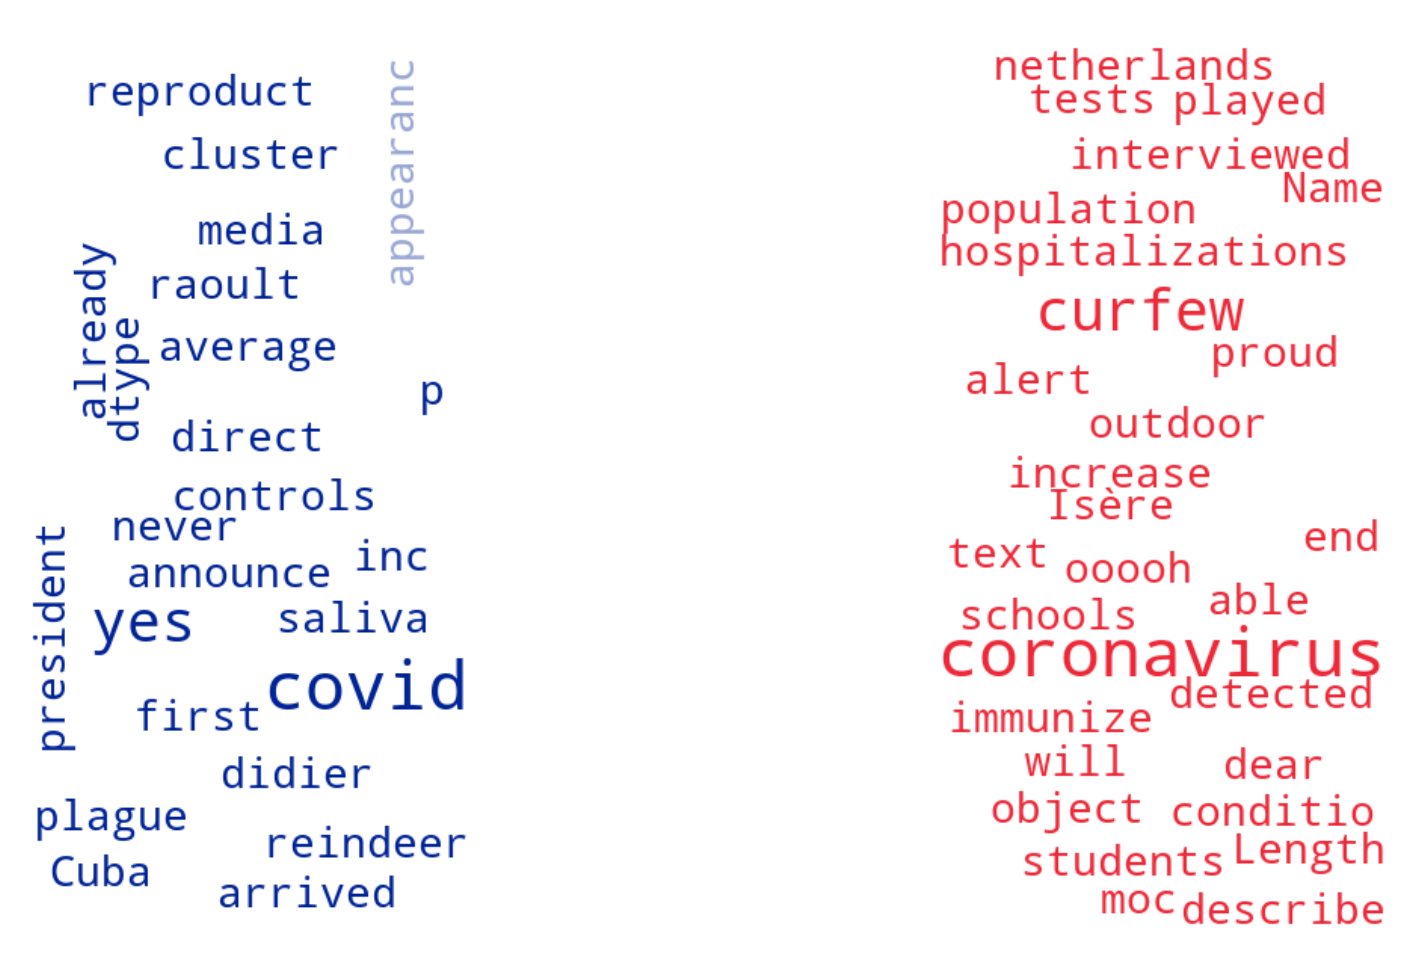
\includegraphics[width=\linewidth]{February fr word cloud.png}
  \caption{French word cloud in February}\label{fig:februaryfr}
\endminipage
\end{figure}
\begin{figure}[!htb]
\minipage{0.33\textwidth}
  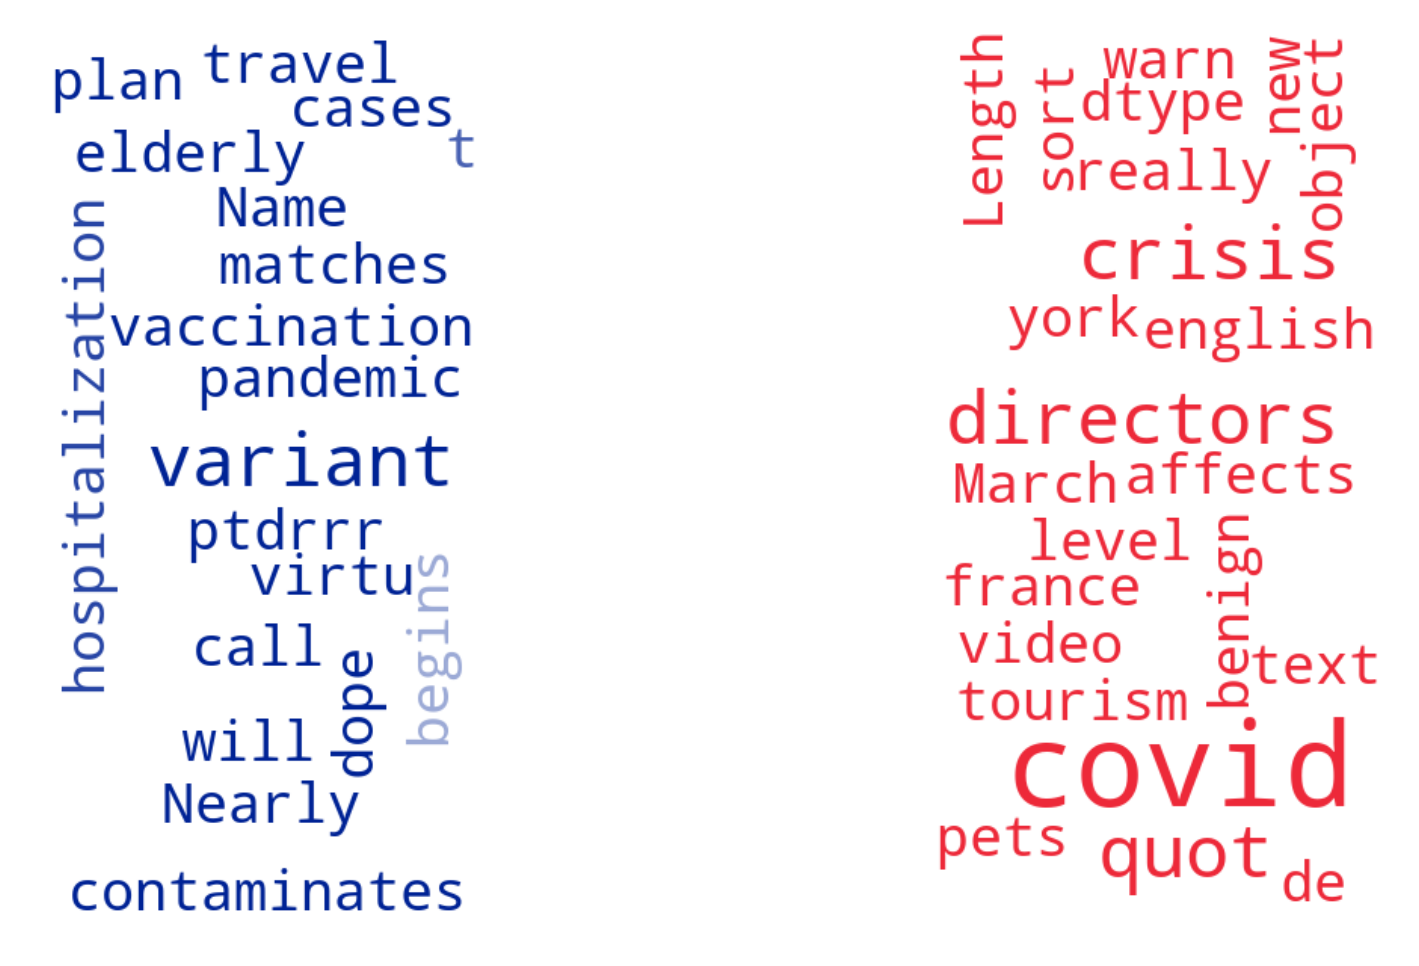
\includegraphics[width=\linewidth]{March fr word cloud.png}
  \caption{French word cloud in March}\label{fig:marchfr}
\endminipage\hfill
\minipage{0.33\textwidth}
  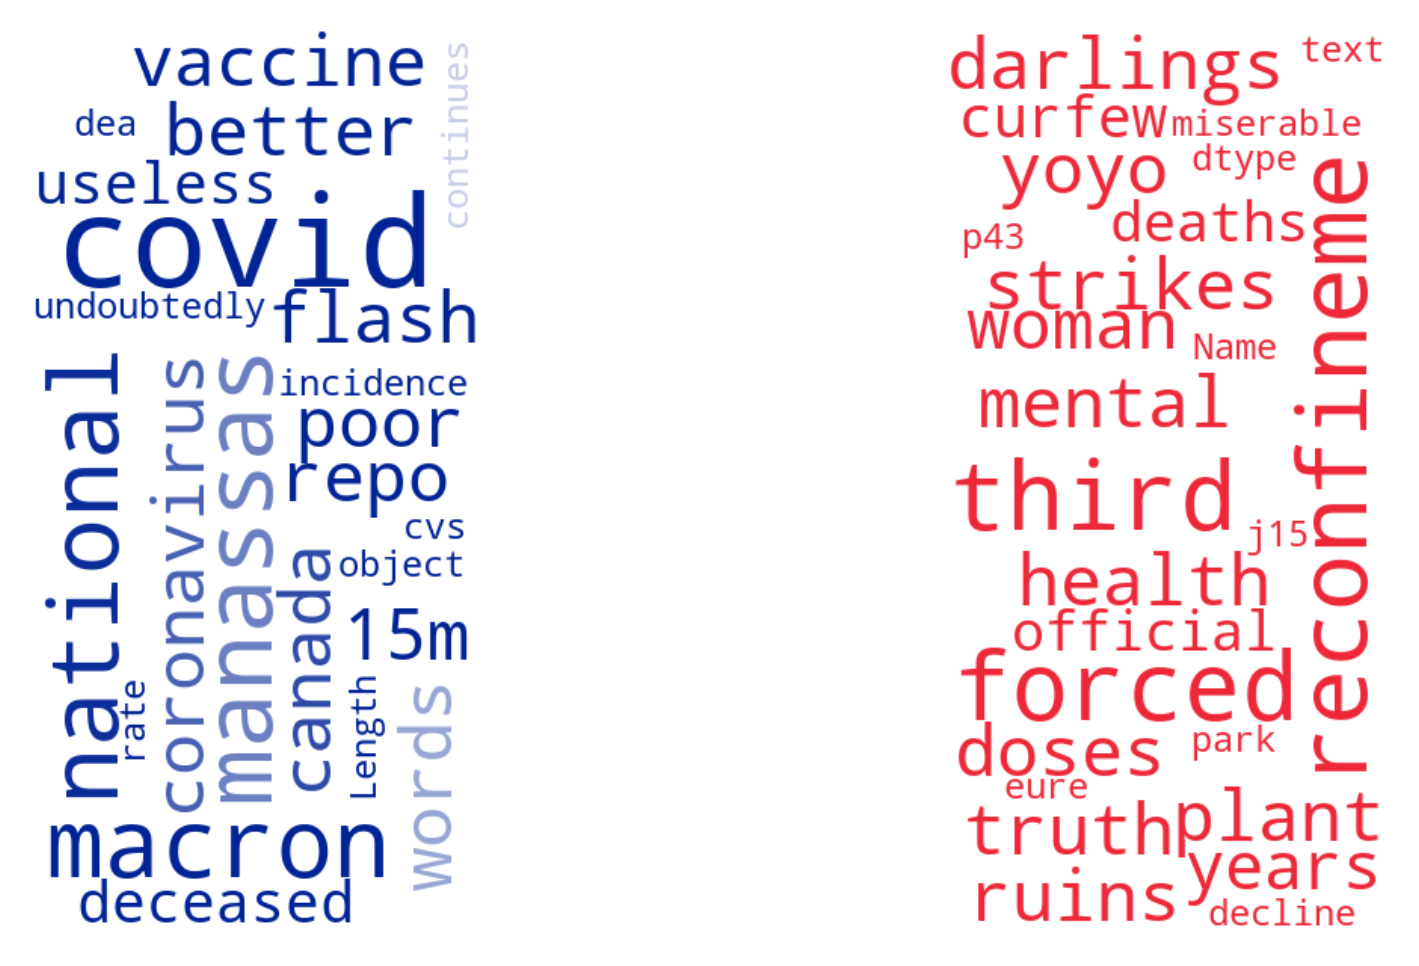
\includegraphics[width=\linewidth]{April fr word cloud.png}
  \caption{French word cloud in April}\label{fig:aprilfr}
\endminipage\hfill
\minipage{0.33\textwidth}
  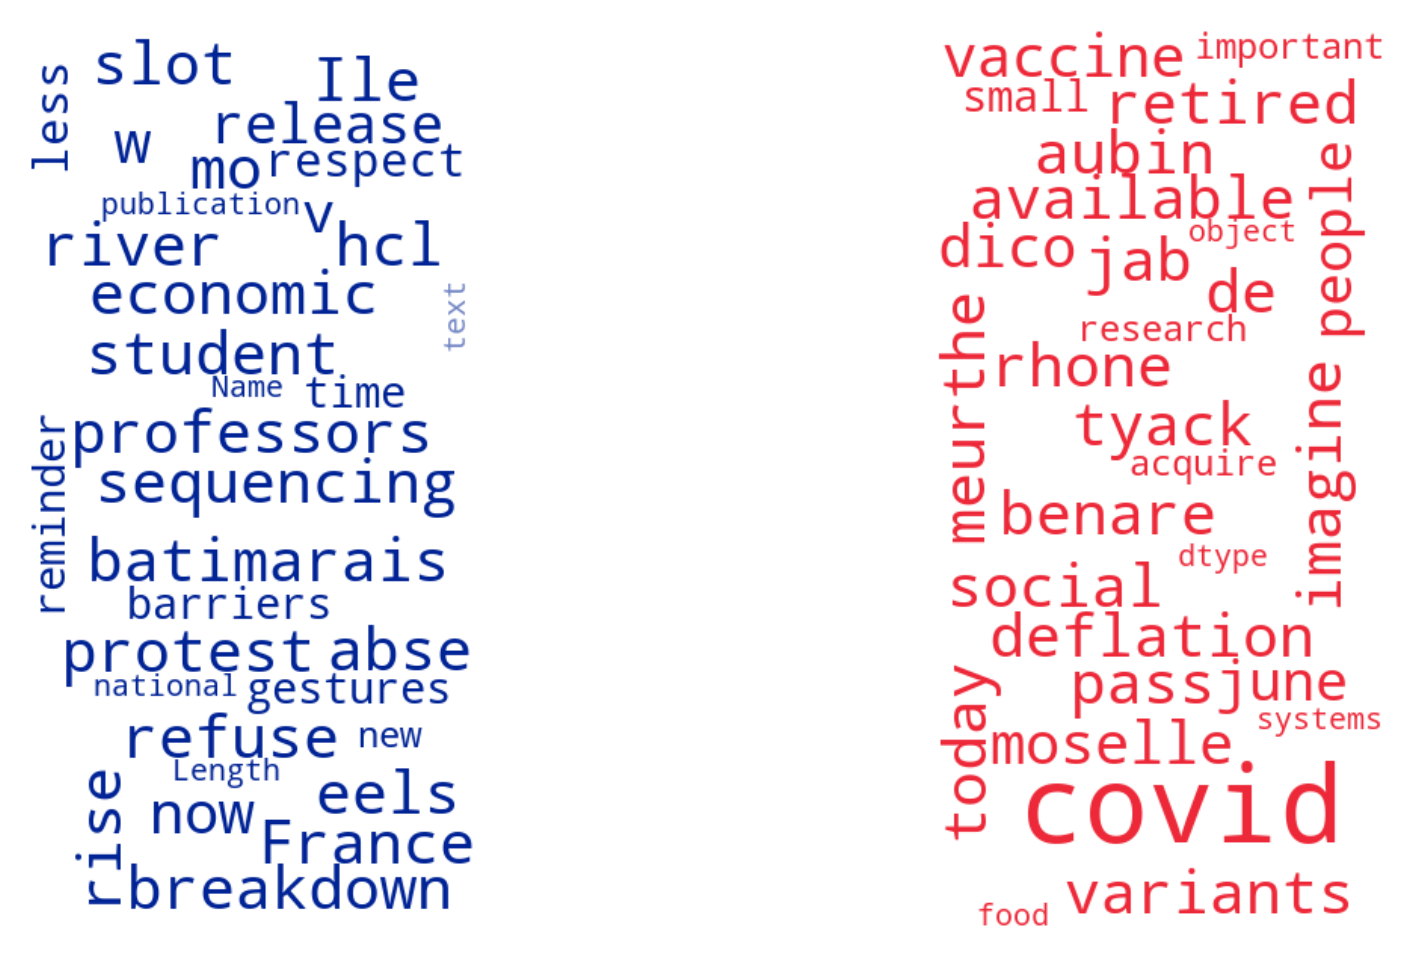
\includegraphics[width=\linewidth]{May fr word cloud.png}
  \caption{French word cloud in May}\label{fig:mayfr}
\endminipage
\end{figure}


\begin{figure}[!htb]
\minipage{0.33\textwidth}
  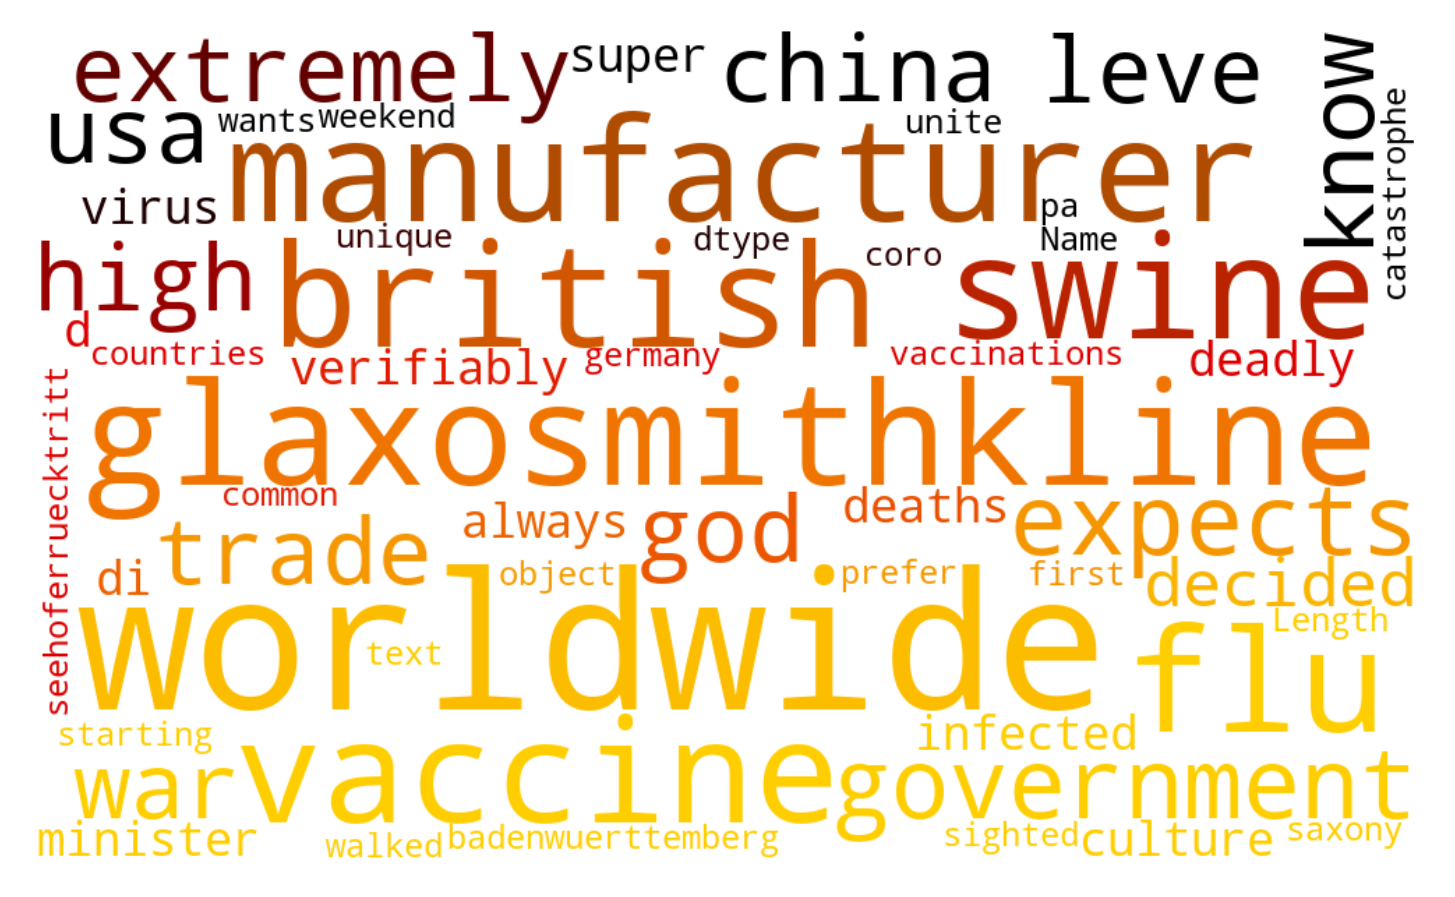
\includegraphics[width=\linewidth]{December de word cloud.png}
  \caption{German word cloud in December}\label{fig:decemberde}
\endminipage\hfill
\minipage{0.33\textwidth}
  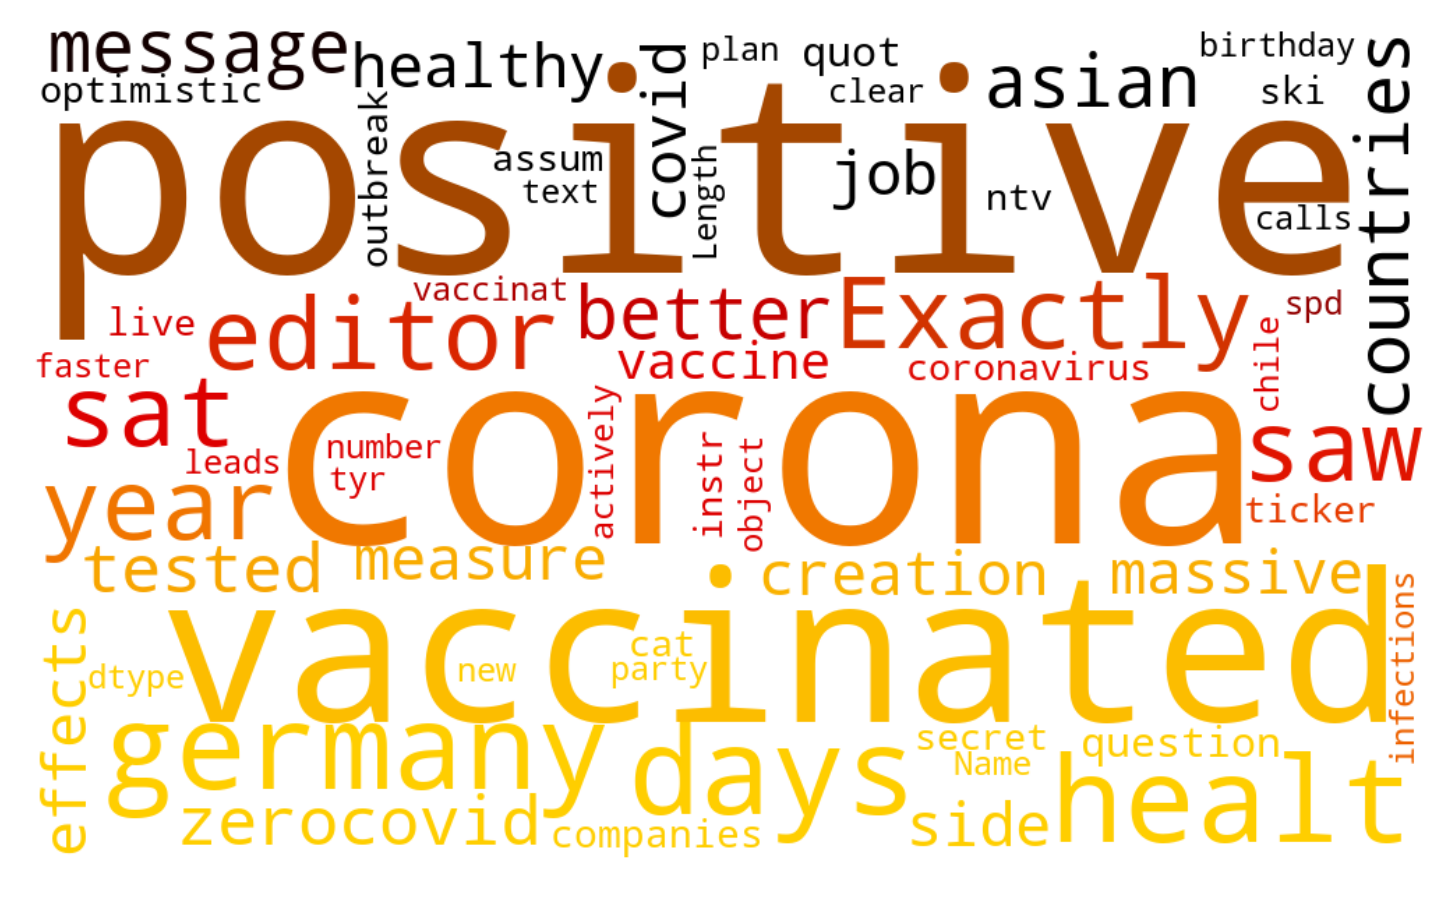
\includegraphics[width=\linewidth]{January de word cloud.png}
  \caption{German word cloud in January}\label{fig:januaryde}
\endminipage\hfill
\minipage{0.33\textwidth}
  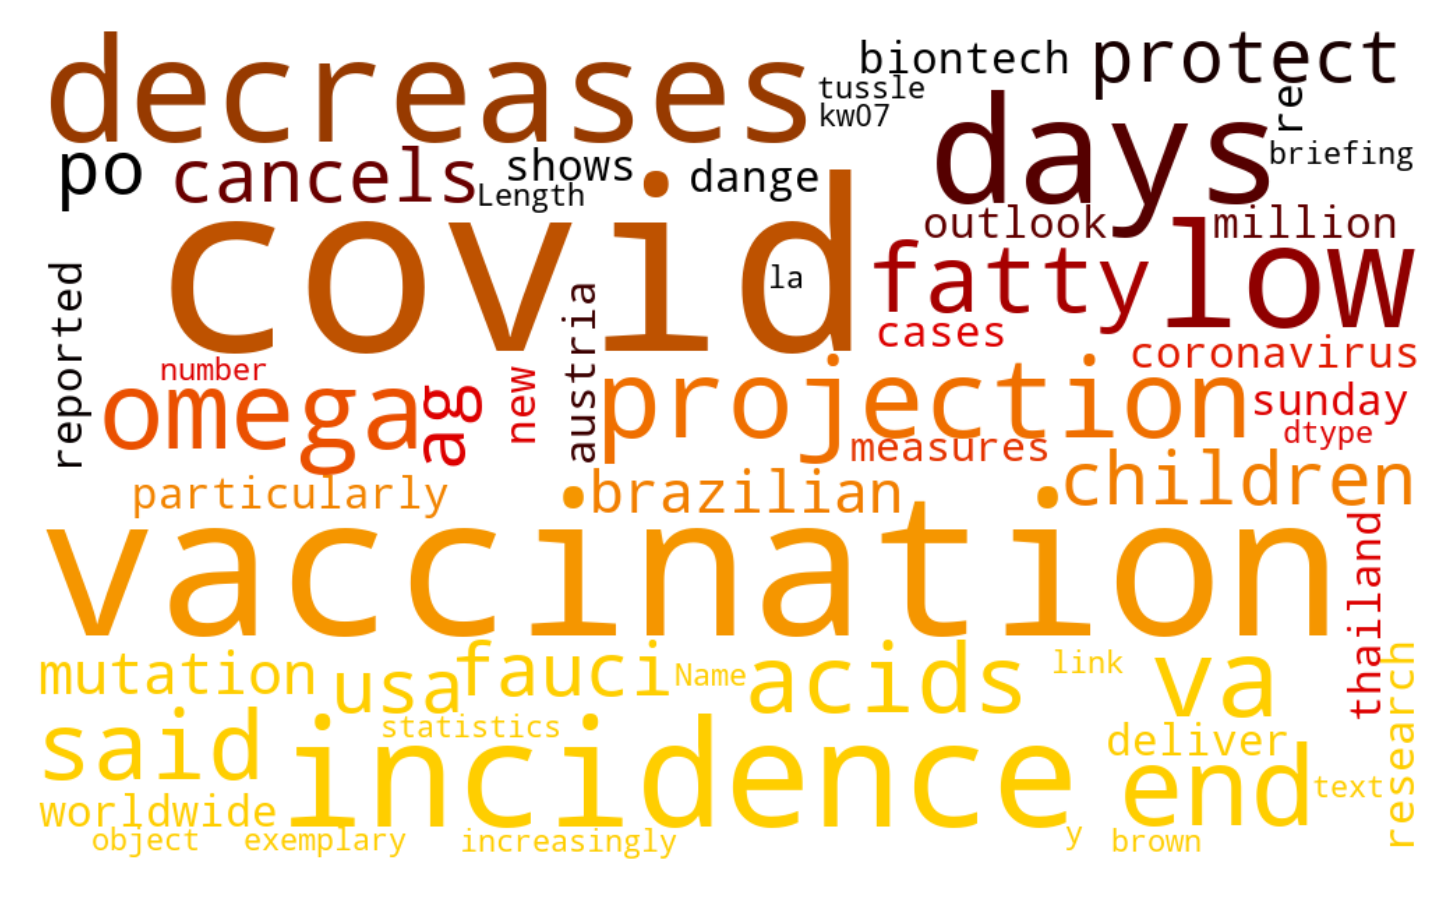
\includegraphics[width=\linewidth]{February de word cloud.png}
  \caption{German word cloud in February}\label{fig:februaryde}
\endminipage
\end{figure}
\begin{figure}[!htb]
\minipage{0.33\textwidth}
  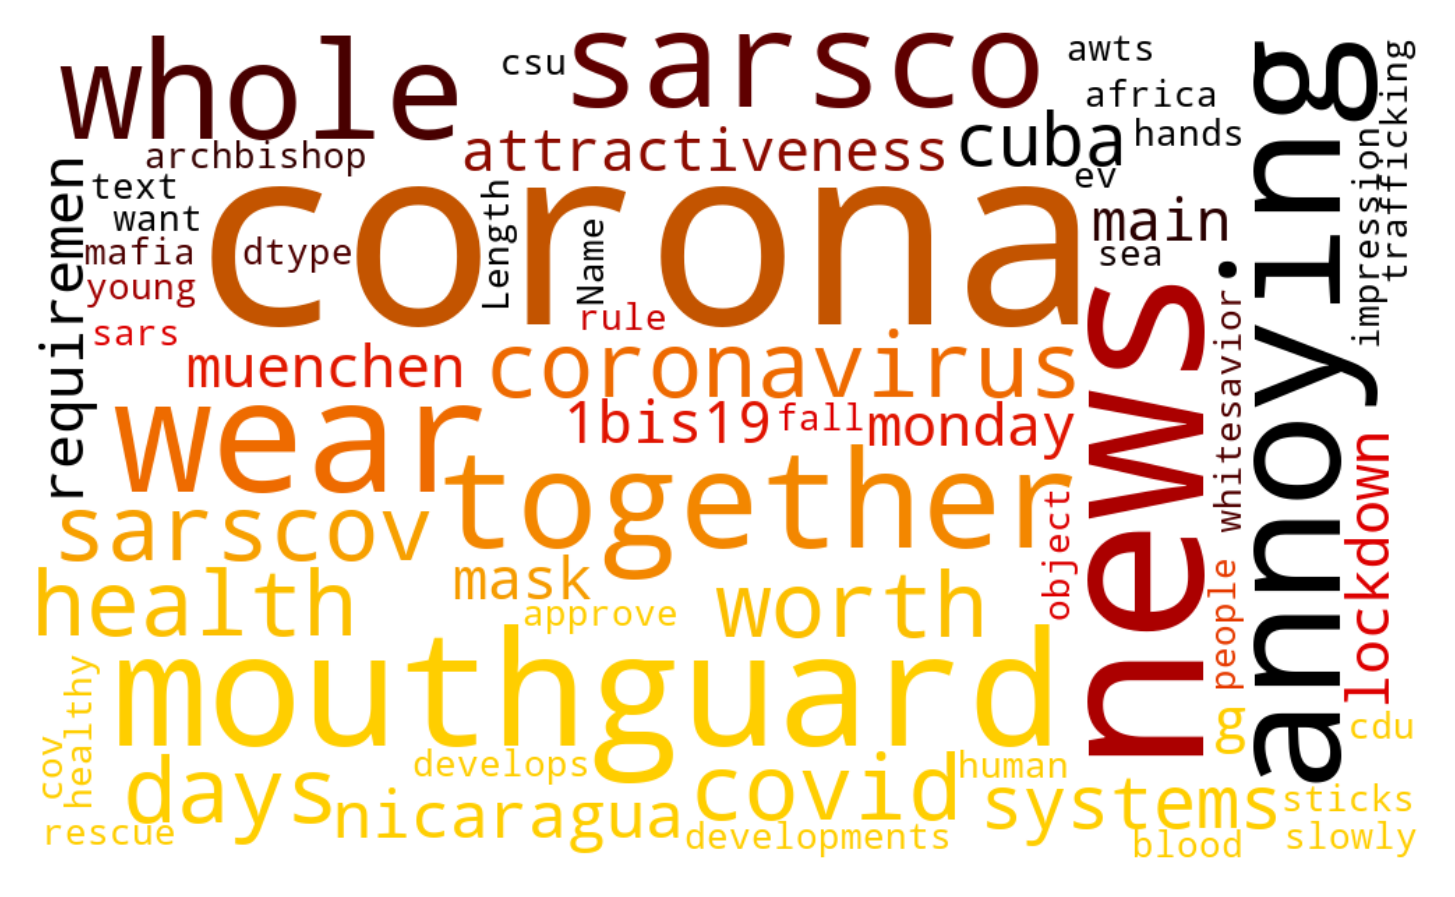
\includegraphics[width=\linewidth]{March de word cloud.png}
  \caption{German word cloud in March}\label{fig:marchde}
\endminipage\hfill
\minipage{0.33\textwidth}
  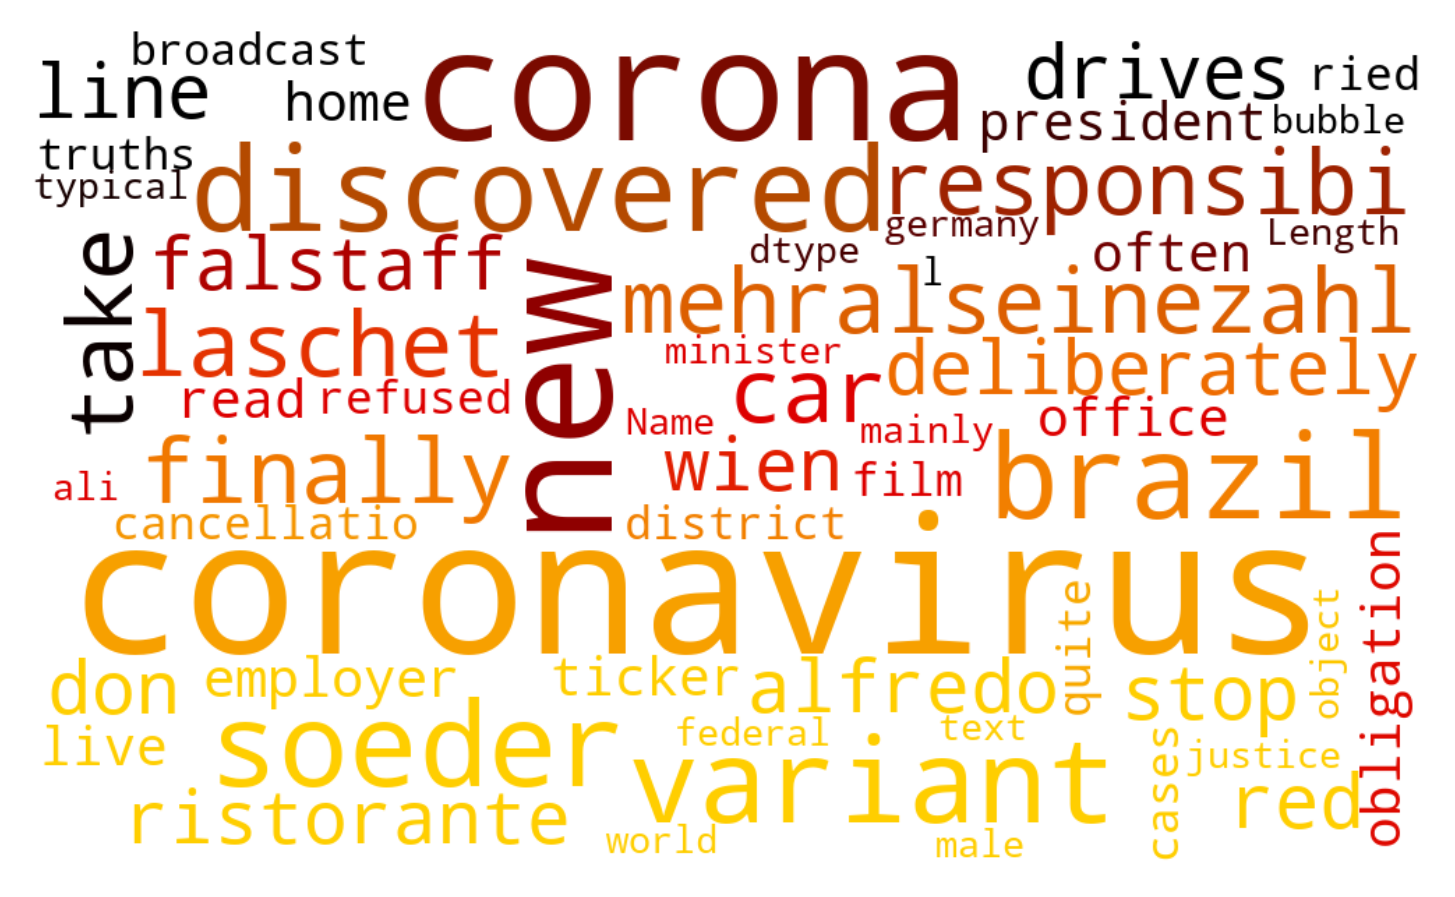
\includegraphics[width=\linewidth]{April de word cloud.png}
  \caption{German word cloud in April}\label{fig:aprilde}
\endminipage\hfill
\minipage{0.33\textwidth}
  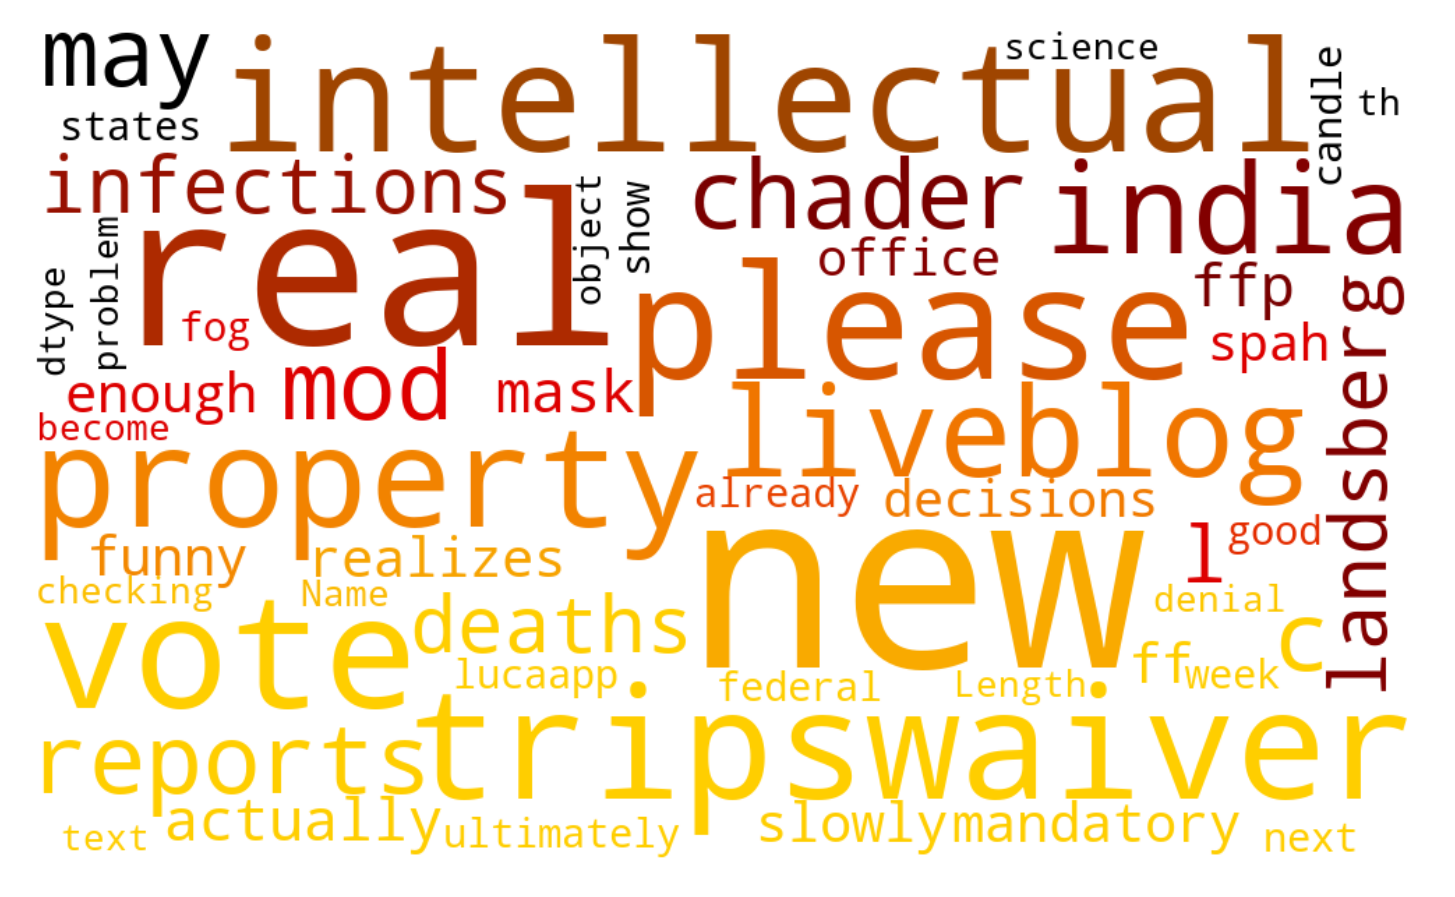
\includegraphics[width=\linewidth]{May de word cloud.png}
  \caption{German word cloud in May}\label{fig:mayde}
\endminipage
\end{figure}


\begin{figure}[!htb]
\minipage{0.33\textwidth}
  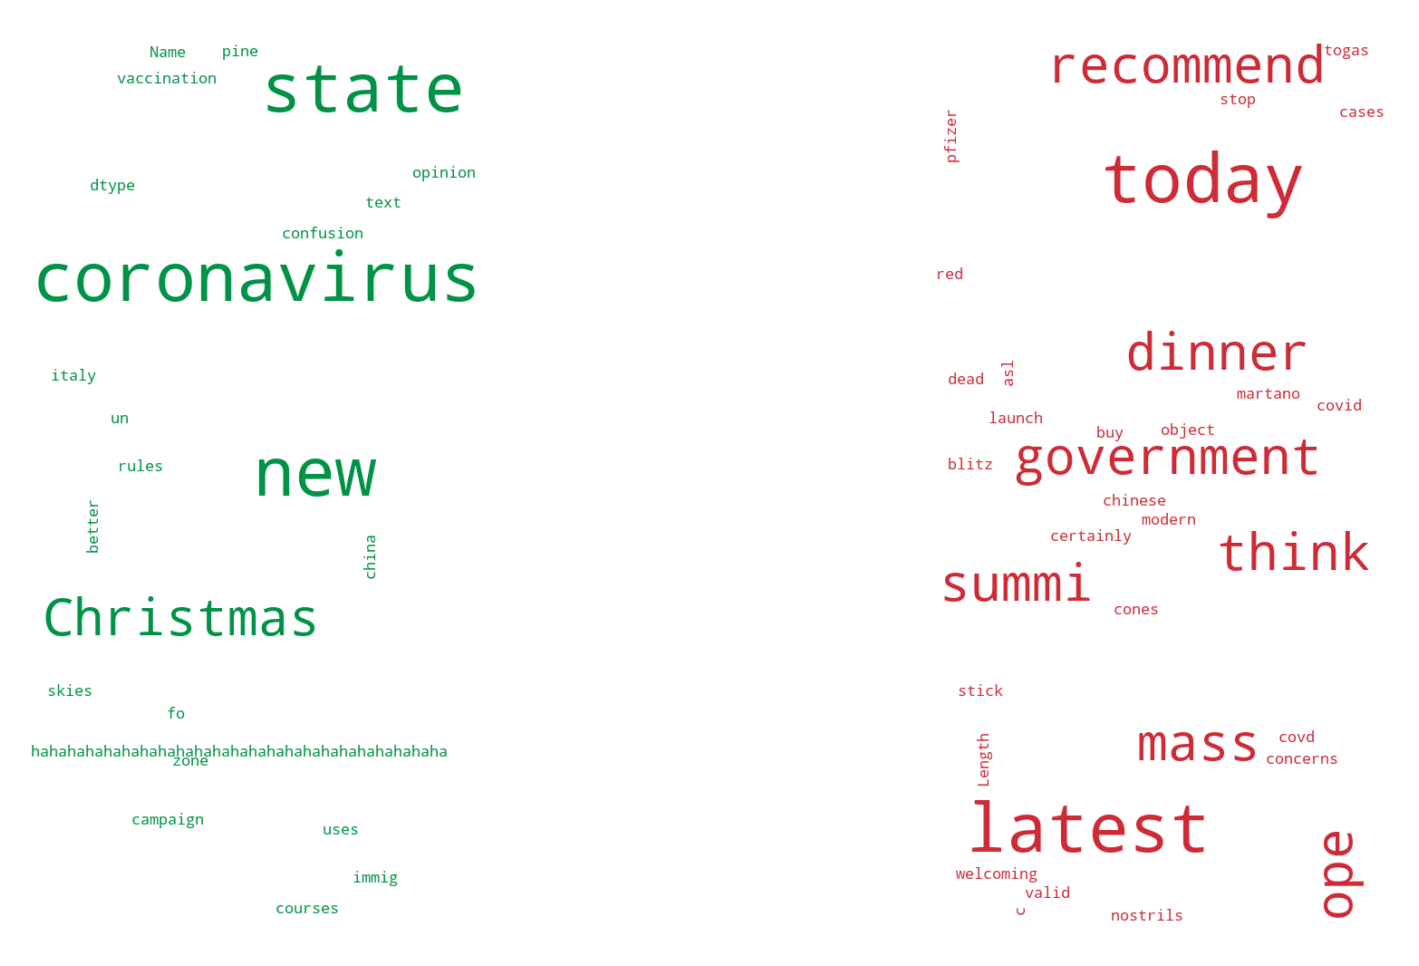
\includegraphics[width=\linewidth]{December it word cloud.png}
  \caption{Italian word cloud in December}\label{fig:decemberit}
\endminipage\hfill
\minipage{0.33\textwidth}
  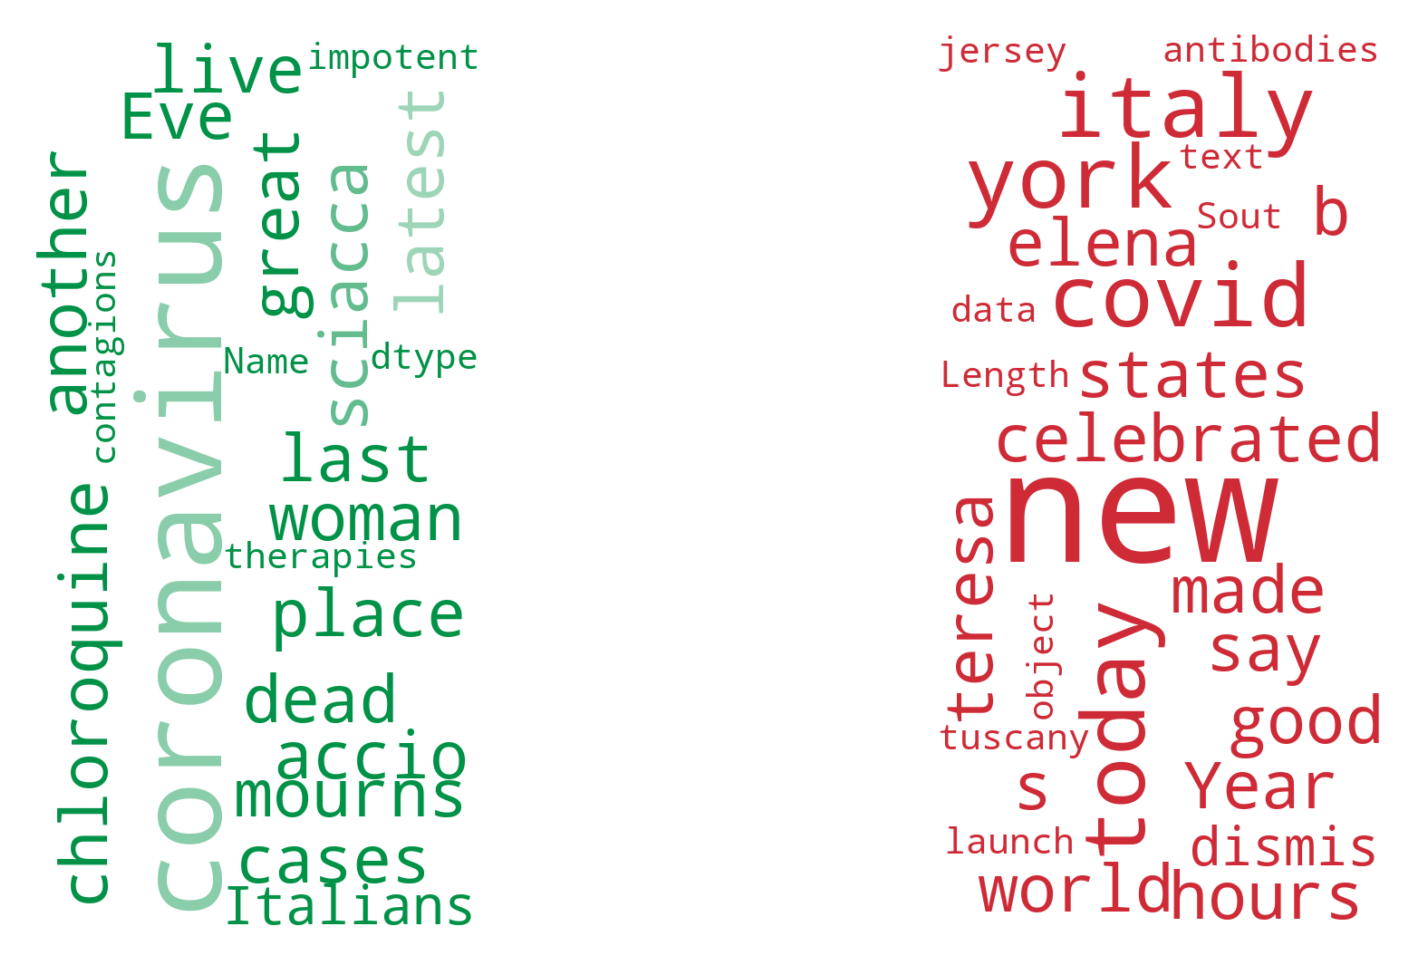
\includegraphics[width=\linewidth]{January it word cloud.png}
  \caption{Italian word cloud in January}\label{fig:januaryit}
\endminipage\hfill
\minipage{0.33\textwidth}
  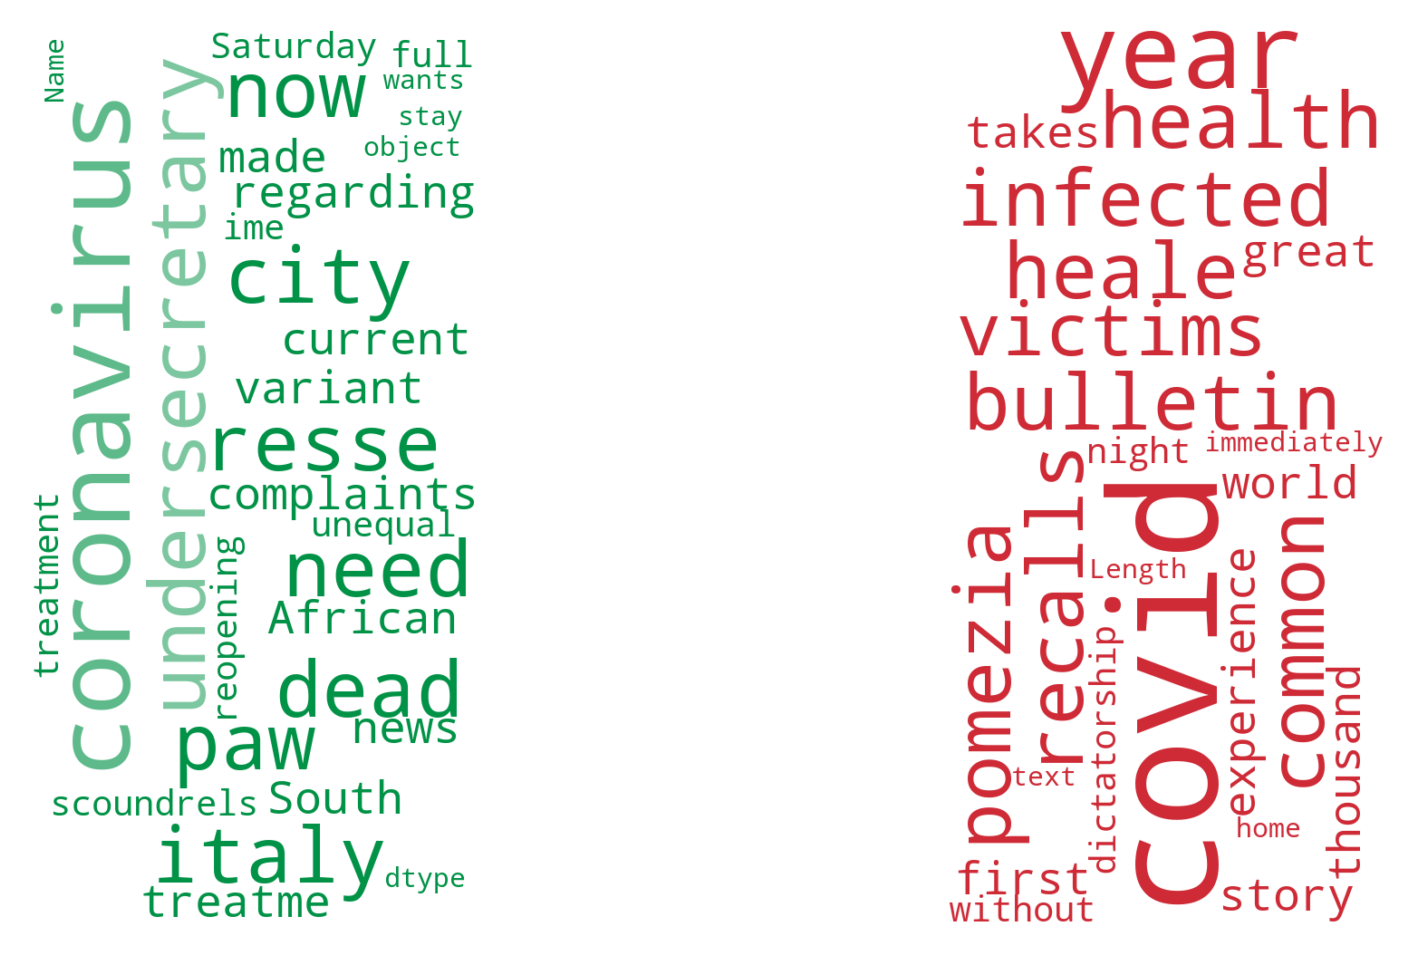
\includegraphics[width=\linewidth]{February it word cloud.png}
  \caption{Italian word cloud in February}\label{fig:februaryit}
\endminipage
\end{figure}
\begin{figure}[!htb]
\minipage{0.33\textwidth}
  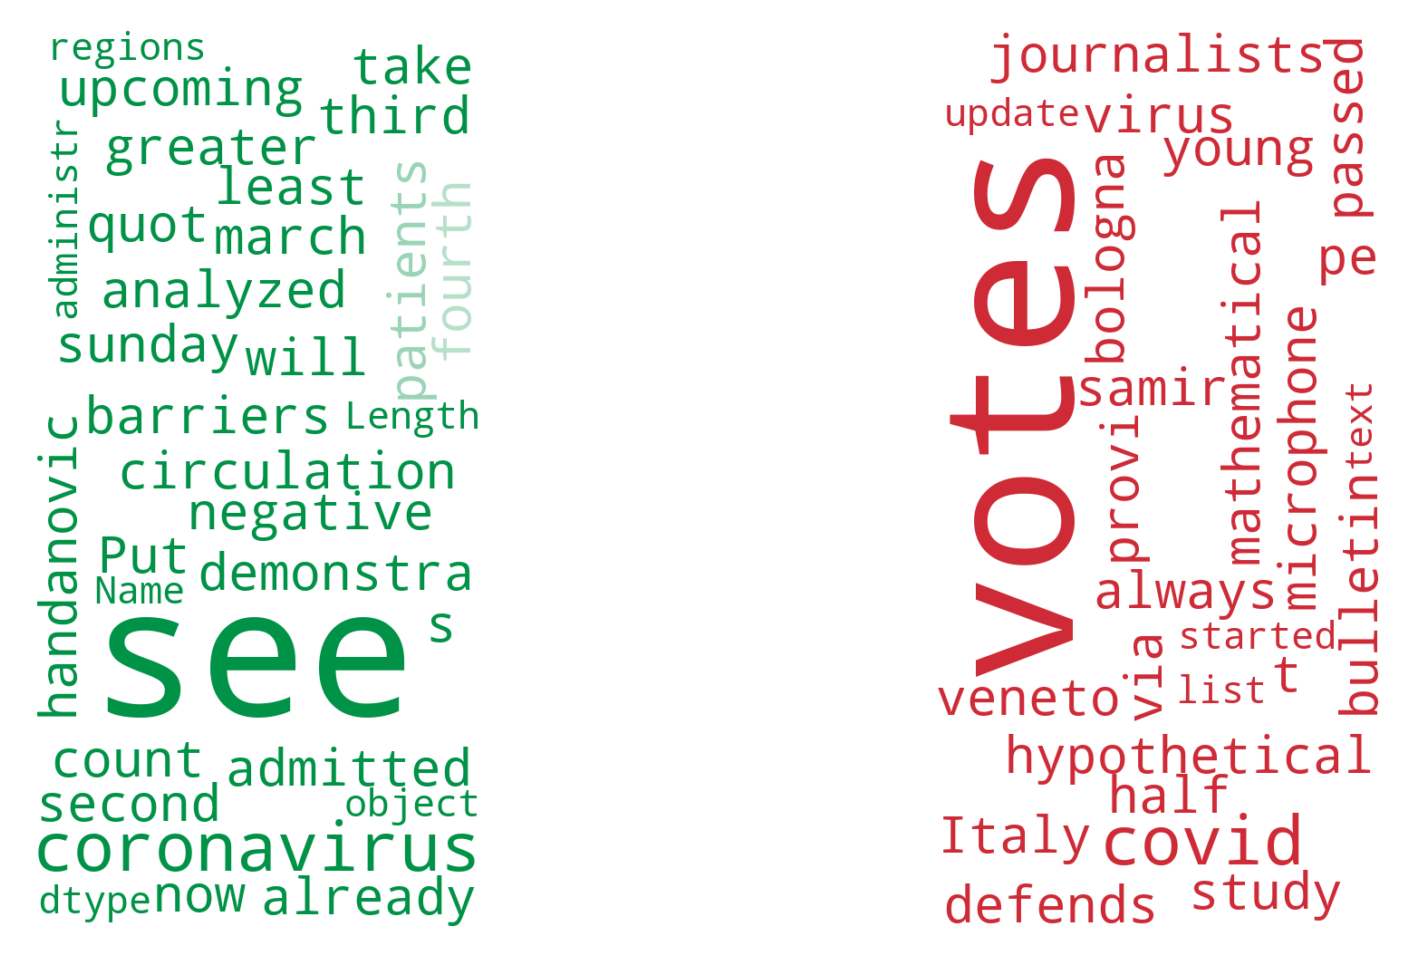
\includegraphics[width=\linewidth]{March it word cloud.png}
  \caption{Italian word cloud in March}\label{fig:marchit}
\endminipage\hfill
\minipage{0.33\textwidth}
  \includegraphics[width=\linewidth]{April it word cloud.png}
  \caption{Italian word cloud in April}\label{fig:aprilit}
\endminipage\hfill
\minipage{0.33\textwidth}
  \includegraphics[width=\linewidth]{May it word cloud.png}
  \caption{Italian word cloud in May}\label{fig:mayit}
\endminipage
\end{figure}


\begin{figure}[!htb]
\minipage{0.33\textwidth}
  \includegraphics[width=\linewidth]{December nl word cloud.png}
  \caption{Dutch word cloud in December}\label{fig:decembernl}
\endminipage\hfill
\minipage{0.33\textwidth}
  \includegraphics[width=\linewidth]{January nl word cloud.png}
  \caption{Dutch word cloud in January}\label{fig:januarynl}
\endminipage\hfill
\minipage{0.33\textwidth}
  \includegraphics[width=\linewidth]{February nl word cloud.png}
  \caption{Dutch word cloud in February}\label{fig:februarynl}
\endminipage
\end{figure}
\begin{figure}[!htb]
\minipage{0.33\textwidth}
  \includegraphics[width=\linewidth]{March nl word cloud.png}
  \caption{Dutch word cloud in March}\label{fig:marchnl}
\endminipage\hfill
\minipage{0.33\textwidth}
  \includegraphics[width=\linewidth]{April nl word cloud.png}
  \caption{Dutch word cloud in April}\label{fig:aprilnl}
\endminipage\hfill
\minipage{0.33\textwidth}
  \includegraphics[width=\linewidth]{May nl word cloud.png}
  \caption{Dutch word cloud in May}\label{fig:maynl}
\endminipage
\end{figure}

\end{landscape}
